\documentclass[aspectratio=1610]{beamer}
\usetheme{bjeldbak}
\usepackage{xspace}
\usepackage{graphicx}
\usepackage{textpos}
\usepackage{subfigure}
\usepackage{pifont}
\usepackage[super]{nth}
\usepackage{relsize}
\usepackage{amsmath}
\usepackage{bm}

\setbeamertemplate{section page}{
  \begin{centering}
    \begin{beamercolorbox}[sep=12pt,center]{part title}
      \huge
      \insertsection
    \end{beamercolorbox}
  \end{centering}
}

\definecolor{anti-flashwhite}{rgb}{0.95, 0.95, 0.96}

\setbeamercolor{section in toc}{fg=anti-flashwhite}

\setbeamertemplate{section page}{
  \begin{centering}
    \begin{beamercolorbox}[sep=12pt,center]{part title}
      \huge
      \insertsection
    \end{beamercolorbox}
  \end{centering}
}

\usepackage{ifthen}
\usepackage{mciteplus} 
\newboolean{uprightparticles}
\setboolean{uprightparticles}{false} %Set true for upright particle symbols
\usepackage{xspace} 
\usepackage{upgreek}

%%% $Id: lhcb-symbols-def.tex 82618 2015-10-14 14:53:43Z pkoppenb $
%%% ======================================================================
%%% Purpose: Standard LHCb aliases
%%% Author: Originally Ulrik Egede, adapted by Tomasz Skwarnicki for templates,
%%% rewritten by Chris Parkes
%%% Maintainer : Ulrik Egede (2010 - 2012)
%%% Maintainer : Rolf Oldeman (2012 - 2014)
%%% =======================================================================

%%% To use this file outside the normal LHCb document environment, the
%%% following should be added in a preamble (before \begin{document}
%%%
%%%\usepackage{ifthen} 
%%%\newboolean{uprightparticles}
%%%\setboolean{uprightparticles}{false} %Set true for upright particle symbols
\usepackage{xspace} 
\usepackage{upgreek}

%%%%%%%%%%%%%%%%%%%%%%%%%%%%%%%%%%%%%%%%%%%%%%%%%%%%%%%%%%%%
%%%
%%% The following is to ensure that the template automatically can process
%%% this file.
%%%
%%% Add comments with at least three %%% preceding.
%%% Add new sections with one % preceding
%%% Add new subsections with two %% preceding
%%%%%%%%%%%%%%%%%%%%%%%%%%%%%%%%%%%%%%%%%%%%%%%%%%%%%%%%%%%%

%%%%%%%%%%%%%
% Experiments
%%%%%%%%%%%%%
\def\lhcb {\mbox{LHCb}\xspace}
\def\atlas  {\mbox{ATLAS}\xspace}
\def\cms    {\mbox{CMS}\xspace}
\def\alice  {\mbox{ALICE}\xspace}
\def\babar  {\mbox{BaBar}\xspace}
\def\belle  {\mbox{Belle}\xspace}
\def\cleo   {\mbox{CLEO}\xspace}
\def\cdf    {\mbox{CDF}\xspace}
\def\dzero  {\mbox{D0}\xspace}
\def\aleph  {\mbox{ALEPH}\xspace}
\def\delphi {\mbox{DELPHI}\xspace}
\def\opal   {\mbox{OPAL}\xspace}
\def\lthree {\mbox{L3}\xspace}
\def\sld    {\mbox{SLD}\xspace}
%%%\def\argus  {\mbox{ARGUS}\xspace}
%%%\def\uaone  {\mbox{UA1}\xspace}
%%%\def\uatwo  {\mbox{UA2}\xspace}
%%%\def\ux85 {\mbox{UX85}\xspace}
\def\cern {\mbox{CERN}\xspace}
\def\lhc    {\mbox{LHC}\xspace}
\def\lep    {\mbox{LEP}\xspace}
\def\tevatron {Tevatron\xspace}

%% LHCb sub-detectors and sub-systems

%%%\def\pu     {PU\xspace}
\def\velo   {VELO\xspace}
\def\rich   {RICH\xspace}
\def\richone {RICH1\xspace}
\def\richtwo {RICH2\xspace}
\def\ttracker {TT\xspace}
\def\intr   {IT\xspace}
\def\st     {ST\xspace}
\def\ot     {OT\xspace}
%%%\def\Tone   {T1\xspace}
%%%\def\Ttwo   {T2\xspace}
%%%\def\Tthree {T3\xspace}
%%%\def\Mone   {M1\xspace}
%%%\def\Mtwo   {M2\xspace}
%%%\def\Mthree {M3\xspace}
%%%\def\Mfour  {M4\xspace}
%%%\def\Mfive  {M5\xspace}
\def\spd    {SPD\xspace}
\def\presh  {PS\xspace}
\def\ecal   {ECAL\xspace}
\def\hcal   {HCAL\xspace}
%%%\def\bcm    {BCM\xspace}
\def\MagUp {\mbox{\em Mag\kern -0.05em Up}\xspace}
\def\MagDown {\mbox{\em MagDown}\xspace}

\def\ode    {ODE\xspace}
\def\daq    {DAQ\xspace}
\def\tfc    {TFC\xspace}
\def\ecs    {ECS\xspace}
\def\lone   {L0\xspace}
\def\hlt    {HLT\xspace}
\def\hltone {HLT1\xspace}
\def\hlttwo {HLT2\xspace}

%%% Upright (not slanted) Particles

\ifthenelse{\boolean{uprightparticles}}%
{\def\Palpha      {\ensuremath{\upalpha}\xspace}
 \def\Pbeta       {\ensuremath{\upbeta}\xspace}
 \def\Pgamma      {\ensuremath{\upgamma}\xspace}                 
 \def\Pdelta      {\ensuremath{\updelta}\xspace}                 
 \def\Pepsilon    {\ensuremath{\upepsilon}\xspace}                 
 \def\Pvarepsilon {\ensuremath{\upvarepsilon}\xspace}                 
 \def\Pzeta       {\ensuremath{\upzeta}\xspace}                 
 \def\Peta        {\ensuremath{\upeta}\xspace}                 
 \def\Ptheta      {\ensuremath{\uptheta}\xspace}                 
 \def\Pvartheta   {\ensuremath{\upvartheta}\xspace}                 
 \def\Piota       {\ensuremath{\upiota}\xspace}                 
 \def\Pkappa      {\ensuremath{\upkappa}\xspace}                 
 \def\Plambda     {\ensuremath{\uplambda}\xspace}                 
 \def\Pmu         {\ensuremath{\upmu}\xspace}                 
 \def\Pnu         {\ensuremath{\upnu}\xspace}                 
 \def\Pxi         {\ensuremath{\upxi}\xspace}                 
 \def\Ppi         {\ensuremath{\uppi}\xspace}                 
 \def\Pvarpi      {\ensuremath{\upvarpi}\xspace}                 
 \def\Prho        {\ensuremath{\uprho}\xspace}                 
 \def\Pvarrho     {\ensuremath{\upvarrho}\xspace}                 
 \def\Ptau        {\ensuremath{\uptau}\xspace}                 
 \def\Pupsilon    {\ensuremath{\upupsilon}\xspace}                 
 \def\Pphi        {\ensuremath{\upphi}\xspace}                 
 \def\Pvarphi     {\ensuremath{\upvarphi}\xspace}                 
 \def\Pchi        {\ensuremath{\upchi}\xspace}                 
 \def\Ppsi        {\ensuremath{\uppsi}\xspace}                 
 \def\Pomega      {\ensuremath{\upomega}\xspace}                 

 \def\PDelta      {\ensuremath{\Delta}\xspace}                 
 \def\PXi      {\ensuremath{\Xi}\xspace}                 
 \def\PLambda      {\ensuremath{\Lambda}\xspace}                 
 \def\PSigma      {\ensuremath{\Sigma}\xspace}                 
 \def\POmega      {\ensuremath{\Omega}\xspace}                 
 \def\PUpsilon      {\ensuremath{\Upsilon}\xspace}                 
 
 %\mathchardef\Deltares="7101
 %\mathchardef\Xi="7104
 %\mathchardef\Lambda="7103
 %\mathchardef\Sigma="7106
 %\mathchardef\Omega="710A


 \def\PA      {\ensuremath{\mathrm{A}}\xspace}                 
 \def\PB      {\ensuremath{\mathrm{B}}\xspace}                 
 \def\PC      {\ensuremath{\mathrm{C}}\xspace}                 
 \def\PD      {\ensuremath{\mathrm{D}}\xspace}                 
 \def\PE      {\ensuremath{\mathrm{E}}\xspace}                 
 \def\PF      {\ensuremath{\mathrm{F}}\xspace}                 
 \def\PG      {\ensuremath{\mathrm{G}}\xspace}                 
 \def\PH      {\ensuremath{\mathrm{H}}\xspace}                 
 \def\PI      {\ensuremath{\mathrm{I}}\xspace}                 
 \def\PJ      {\ensuremath{\mathrm{J}}\xspace}                 
 \def\PK      {\ensuremath{\mathrm{K}}\xspace}                 
 \def\PL      {\ensuremath{\mathrm{L}}\xspace}                 
 \def\PM      {\ensuremath{\mathrm{M}}\xspace}                 
 \def\PN      {\ensuremath{\mathrm{N}}\xspace}                 
 \def\PO      {\ensuremath{\mathrm{O}}\xspace}                 
 \def\PP      {\ensuremath{\mathrm{P}}\xspace}                 
 \def\PQ      {\ensuremath{\mathrm{Q}}\xspace}                 
 \def\PR      {\ensuremath{\mathrm{R}}\xspace}                 
 \def\PS      {\ensuremath{\mathrm{S}}\xspace}                 
 \def\PT      {\ensuremath{\mathrm{T}}\xspace}                 
 \def\PU      {\ensuremath{\mathrm{U}}\xspace}                 
 \def\PV      {\ensuremath{\mathrm{V}}\xspace}                 
 \def\PW      {\ensuremath{\mathrm{W}}\xspace}                 
 \def\PX      {\ensuremath{\mathrm{X}}\xspace}                 
 \def\PY      {\ensuremath{\mathrm{Y}}\xspace}                 
 \def\PZ      {\ensuremath{\mathrm{Z}}\xspace}                 
 \def\Pa      {\ensuremath{\mathrm{a}}\xspace}                 
 \def\Pb      {\ensuremath{\mathrm{b}}\xspace}                 
 \def\Pc      {\ensuremath{\mathrm{c}}\xspace}                 
 \def\Pd      {\ensuremath{\mathrm{d}}\xspace}                 
 \def\Pe      {\ensuremath{\mathrm{e}}\xspace}                 
 \def\Pf      {\ensuremath{\mathrm{f}}\xspace}                 
 \def\Pg      {\ensuremath{\mathrm{g}}\xspace}                 
 \def\Ph      {\ensuremath{\mathrm{h}}\xspace}                 
 \def\Pi      {\ensuremath{\mathrm{i}}\xspace}                 
 \def\Pj      {\ensuremath{\mathrm{j}}\xspace}                 
 \def\Pk      {\ensuremath{\mathrm{k}}\xspace}                 
 \def\Pl      {\ensuremath{\mathrm{l}}\xspace}                 
 \def\Pm      {\ensuremath{\mathrm{m}}\xspace}                 
 \def\Pn      {\ensuremath{\mathrm{n}}\xspace}                 
 \def\Po      {\ensuremath{\mathrm{o}}\xspace}                 
 \def\Pp      {\ensuremath{\mathrm{p}}\xspace}                 
 \def\Pq      {\ensuremath{\mathrm{q}}\xspace}                 
 \def\Pr      {\ensuremath{\mathrm{r}}\xspace}                 
 \def\Ps      {\ensuremath{\mathrm{s}}\xspace}                 
 \def\Pt      {\ensuremath{\mathrm{t}}\xspace}                 
 \def\Pu      {\ensuremath{\mathrm{u}}\xspace}                 
 \def\Pv      {\ensuremath{\mathrm{v}}\xspace}                 
 \def\Pw      {\ensuremath{\mathrm{w}}\xspace}                 
 \def\Px      {\ensuremath{\mathrm{x}}\xspace}                 
 \def\Py      {\ensuremath{\mathrm{y}}\xspace}                 
 \def\Pz      {\ensuremath{\mathrm{z}}\xspace}                 
}
{\def\Palpha      {\ensuremath{\alpha}\xspace}
 \def\Pbeta       {\ensuremath{\beta}\xspace}
 \def\Pgamma      {\ensuremath{\gamma}\xspace}                 
 \def\Pdelta      {\ensuremath{\delta}\xspace}                 
 \def\Pepsilon    {\ensuremath{\epsilon}\xspace}                 
 \def\Pvarepsilon {\ensuremath{\varepsilon}\xspace}                 
 \def\Pzeta       {\ensuremath{\zeta}\xspace}                 
 \def\Peta        {\ensuremath{\eta}\xspace}                 
 \def\Ptheta      {\ensuremath{\theta}\xspace}                 
 \def\Pvartheta   {\ensuremath{\vartheta}\xspace}                 
 \def\Piota       {\ensuremath{\iota}\xspace}                 
 \def\Pkappa      {\ensuremath{\kappa}\xspace}                 
 \def\Plambda     {\ensuremath{\lambda}\xspace}                 
 \def\Pmu         {\ensuremath{\mu}\xspace}                 
 \def\Pnu         {\ensuremath{\nu}\xspace}                 
 \def\Pxi         {\ensuremath{\xi}\xspace}                 
 \def\Ppi         {\ensuremath{\pi}\xspace}                 
 \def\Pvarpi      {\ensuremath{\varpi}\xspace}                 
 \def\Prho        {\ensuremath{\rho}\xspace}                 
 \def\Pvarrho     {\ensuremath{\varrho}\xspace}                 
 \def\Ptau        {\ensuremath{\tau}\xspace}                 
 \def\Pupsilon    {\ensuremath{\upsilon}\xspace}                 
 \def\Pphi        {\ensuremath{\phi}\xspace}                 
 \def\Pvarphi     {\ensuremath{\varphi}\xspace}                 
 \def\Pchi        {\ensuremath{\chi}\xspace}                 
 \def\Ppsi        {\ensuremath{\psi}\xspace}                 
 \def\Pomega      {\ensuremath{\omega}\xspace}                 
 \mathchardef\PDelta="7101
 \mathchardef\PXi="7104
 \mathchardef\PLambda="7103
 \mathchardef\PSigma="7106
 \mathchardef\POmega="710A
 \mathchardef\PUpsilon="7107
 \def\PA      {\ensuremath{A}\xspace}                 
 \def\PB      {\ensuremath{B}\xspace}                 
 \def\PC      {\ensuremath{C}\xspace}                 
 \def\PD      {\ensuremath{D}\xspace}                 
 \def\PE      {\ensuremath{E}\xspace}                 
 \def\PF      {\ensuremath{F}\xspace}                 
 \def\PG      {\ensuremath{G}\xspace}                 
 \def\PH      {\ensuremath{H}\xspace}                 
 \def\PI      {\ensuremath{I}\xspace}                 
 \def\PJ      {\ensuremath{J}\xspace}                 
 \def\PK      {\ensuremath{K}\xspace}                 
 \def\PL      {\ensuremath{L}\xspace}                 
 \def\PM      {\ensuremath{M}\xspace}                 
 \def\PN      {\ensuremath{N}\xspace}                 
 \def\PO      {\ensuremath{O}\xspace}                 
 \def\PP      {\ensuremath{P}\xspace}                 
 \def\PQ      {\ensuremath{Q}\xspace}                 
 \def\PR      {\ensuremath{R}\xspace}                 
 \def\PS      {\ensuremath{S}\xspace}                 
 \def\PT      {\ensuremath{T}\xspace}                 
 \def\PU      {\ensuremath{U}\xspace}                 
 \def\PV      {\ensuremath{V}\xspace}                 
 \def\PW      {\ensuremath{W}\xspace}                 
 \def\PX      {\ensuremath{X}\xspace}                 
 \def\PY      {\ensuremath{Y}\xspace}                 
 \def\PZ      {\ensuremath{Z}\xspace}                 
 \def\Pa      {\ensuremath{a}\xspace}                 
 \def\Pb      {\ensuremath{b}\xspace}                 
 \def\Pc      {\ensuremath{c}\xspace}                 
 \def\Pd      {\ensuremath{d}\xspace}                 
 \def\Pe      {\ensuremath{e}\xspace}                 
 \def\Pf      {\ensuremath{f}\xspace}                 
 \def\Pg      {\ensuremath{g}\xspace}                 
 \def\Ph      {\ensuremath{h}\xspace}                 
 \def\Pi      {\ensuremath{i}\xspace}                 
 \def\Pj      {\ensuremath{j}\xspace}                 
 \def\Pk      {\ensuremath{k}\xspace}                 
 \def\Pl      {\ensuremath{l}\xspace}                 
 \def\Pm      {\ensuremath{m}\xspace}                 
 \def\Pn      {\ensuremath{n}\xspace}                 
 \def\Po      {\ensuremath{o}\xspace}                 
 \def\Pp      {\ensuremath{p}\xspace}                 
 \def\Pq      {\ensuremath{q}\xspace}                 
 \def\Pr      {\ensuremath{r}\xspace}                 
 \def\Ps      {\ensuremath{s}\xspace}                 
 \def\Pt      {\ensuremath{t}\xspace}                 
 \def\Pu      {\ensuremath{u}\xspace}                 
 \def\Pv      {\ensuremath{v}\xspace}                 
 \def\Pw      {\ensuremath{w}\xspace}                 
 \def\Px      {\ensuremath{x}\xspace}                 
 \def\Py      {\ensuremath{y}\xspace}                 
 \def\Pz      {\ensuremath{z}\xspace}                 
}

%%%%%%%%%%%%%%%%%%%%%%%%%%%%%%%%%%%%%%%%%%%%%%%
% Particles
% \makeatletter
% \ifcase \@ptsize \relax% 10pt
%   \newcommand{\miniscule}{\@setfontsize\miniscule{4}{5}}% \tiny: 5/6
% \or% 11pt
%   \newcommand{\miniscule}{\@setfontsize\miniscule{5}{6}}% \tiny: 6/7
% \or% 12pt
%   \newcommand{\miniscule}{\@setfontsize\miniscule{5}{6}}% \tiny: 6/7
% \fi
% \makeatother


\DeclareRobustCommand{\optbar}[1]{\shortstack{{\miniscule (\rule[.5ex]{1.25em}{.18mm})}
  \\ [-.7ex] $#1$}}


%% Leptons

\let\emi\en
\def\electron   {{\ensuremath{\Pe}}\xspace}
\def\en         {{\ensuremath{\Pe^-}}\xspace}   % electron negative (\em is taken)
\def\ep         {{\ensuremath{\Pe^+}}\xspace}
\def\epm        {{\ensuremath{\Pe^\pm}}\xspace} 
\def\epem       {{\ensuremath{\Pe^+\Pe^-}}\xspace}
%%%\def\ee         {\ensuremath{\Pe^-\Pe^-}\xspace}

\def\muon       {{\ensuremath{\Pmu}}\xspace}
\def\mup        {{\ensuremath{\Pmu^+}}\xspace}
\def\mun        {{\ensuremath{\Pmu^-}}\xspace} % muon negative (\mum is taken)
\def\mumu       {{\ensuremath{\Pmu^+\Pmu^-}}\xspace}

\def\tauon      {{\ensuremath{\Ptau}}\xspace}
\def\taup       {{\ensuremath{\Ptau^+}}\xspace}
\def\taum       {{\ensuremath{\Ptau^-}}\xspace}
\def\tautau     {{\ensuremath{\Ptau^+\Ptau^-}}\xspace}

\def\lepton     {{\ensuremath{\ell}}\xspace}
\def\ellm       {{\ensuremath{\ell^-}}\xspace}
\def\ellp       {{\ensuremath{\ell^+}}\xspace}
%%%\def\ellell     {\ensuremath{\ell^+ \ell^-}\xspace}

\def\neu        {{\ensuremath{\Pnu}}\xspace}
\def\neub       {{\ensuremath{\overline{\Pnu}}}\xspace}
%%%\def\nuenueb    {\ensuremath{\neu\neub}\xspace}
\def\neue       {{\ensuremath{\neu_e}}\xspace}
\def\neueb      {{\ensuremath{\neub_e}}\xspace}
%%%\def\neueneueb  {\ensuremath{\neue\neueb}\xspace}
\def\neum       {{\ensuremath{\neu_\mu}}\xspace}
\def\neumb      {{\ensuremath{\neub_\mu}}\xspace}
%%%\def\neumneumb  {\ensuremath{\neum\neumb}\xspace}
\def\neut       {{\ensuremath{\neu_\tau}}\xspace}
\def\neutb      {{\ensuremath{\neub_\tau}}\xspace}
%%%\def\neutneutb  {\ensuremath{\neut\neutb}\xspace}
\def\neul       {{\ensuremath{\neu_\ell}}\xspace}
\def\neulb      {{\ensuremath{\neub_\ell}}\xspace}
%%%\def\neulneulb  {\ensuremath{\neul\neulb}\xspace}

%% Gauge bosons and scalars

\def\g      {{\ensuremath{\Pgamma}}\xspace}
\def\H      {{\ensuremath{\PH^0}}\xspace}
\def\Hp     {{\ensuremath{\PH^+}}\xspace}
\def\Hm     {{\ensuremath{\PH^-}}\xspace}
\def\Hpm    {{\ensuremath{\PH^\pm}}\xspace}
\def\W      {{\ensuremath{\PW}}\xspace}
\def\Wp     {{\ensuremath{\PW^+}}\xspace}
\def\Wm     {{\ensuremath{\PW^-}}\xspace}
\def\Wpm    {{\ensuremath{\PW^\pm}}\xspace}
\def\Z      {{\ensuremath{\PZ}}\xspace}

%% Quarks

\def\quark     {{\ensuremath{\Pq}}\xspace}
\def\quarkbar  {{\ensuremath{\overline \quark}}\xspace}
\def\qqbar     {{\ensuremath{\quark\quarkbar}}\xspace}
\def\uquark    {{\ensuremath{\Pu}}\xspace}
\def\uquarkbar {{\ensuremath{\overline \uquark}}\xspace}
\def\uubar     {{\ensuremath{\uquark\uquarkbar}}\xspace}
\def\dquark    {{\ensuremath{\Pd}}\xspace}
\def\dquarkbar {{\ensuremath{\overline \dquark}}\xspace}
\def\ddbar     {{\ensuremath{\dquark\dquarkbar}}\xspace}
\def\squark    {{\ensuremath{\Ps}}\xspace}
\def\squarkbar {{\ensuremath{\overline \squark}}\xspace}
\def\ssbar     {{\ensuremath{\squark\squarkbar}}\xspace}
\def\cquark    {{\ensuremath{\Pc}}\xspace}
\def\cquarkbar {{\ensuremath{\overline \cquark}}\xspace}
\def\ccbar     {{\ensuremath{\cquark\cquarkbar}}\xspace}
\def\bquark    {{\ensuremath{\Pb}}\xspace}
\def\bquarkbar {{\ensuremath{\overline \bquark}}\xspace}
\def\bbbar     {{\ensuremath{\bquark\bquarkbar}}\xspace}
\def\tquark    {{\ensuremath{\Pt}}\xspace}
\def\tquarkbar {{\ensuremath{\overline \tquark}}\xspace}
\def\ttbar     {{\ensuremath{\tquark\tquarkbar}}\xspace}

%% Light mesons

\def\hadron {{\ensuremath{\Ph}}\xspace}
\def\pion   {{\ensuremath{\Ppi}}\xspace}
\def\piz    {{\ensuremath{\pion^0}}\xspace}
\def\pizs   {{\ensuremath{\pion^0\mbox\,\mathrm{s}}}\xspace}
\def\pip    {{\ensuremath{\pion^+}}\xspace}
\def\pim    {{\ensuremath{\pion^-}}\xspace}
\def\pipm   {{\ensuremath{\pion^\pm}}\xspace}
\def\pimp   {{\ensuremath{\pion^\mp}}\xspace}

\def\rhomeson {{\ensuremath{\Prho}}\xspace}
\def\rhoz     {{\ensuremath{\rhomeson^0}}\xspace}
\def\rhop     {{\ensuremath{\rhomeson^+}}\xspace}
\def\rhom     {{\ensuremath{\rhomeson^-}}\xspace}
\def\rhopm    {{\ensuremath{\rhomeson^\pm}}\xspace}
\def\rhomp    {{\ensuremath{\rhomeson^\mp}}\xspace}

\def\kaon    {{\ensuremath{\PK}}\xspace}
%%% do NOT use ensuremath here
  \def\Kbar    {{\kern 0.2em\overline{\kern -0.2em \PK}{}}\xspace}
\def\Kb      {{\ensuremath{\Kbar}}\xspace}
\def\KorKbar    {\kern 0.18em\optbar{\kern -0.18em K}{}\xspace}
\def\Kz      {{\ensuremath{\kaon^0}}\xspace}
\def\Kzb     {{\ensuremath{\Kbar{}^0}}\xspace}
\def\Kp      {{\ensuremath{\kaon^+}}\xspace}
\def\Km      {{\ensuremath{\kaon^-}}\xspace}
\def\Kpm     {{\ensuremath{\kaon^\pm}}\xspace}
\def\Kmp     {{\ensuremath{\kaon^\mp}}\xspace}
\def\KS      {{\ensuremath{\kaon^0_{\mathrm{ \scriptscriptstyle S}}}}\xspace}
\def\KL      {{\ensuremath{\kaon^0_{\mathrm{ \scriptscriptstyle L}}}}\xspace}
\def\Kstarz  {{\ensuremath{\kaon^{*0}}}\xspace}
\def\Kstarzb {{\ensuremath{\Kbar{}^{*0}}}\xspace}
\def\Kstar   {{\ensuremath{\kaon^*}}\xspace}
\def\Kstarb  {{\ensuremath{\Kbar{}^*}}\xspace}
\def\Kstarp  {{\ensuremath{\kaon^{*+}}}\xspace}
\def\Kstarm  {{\ensuremath{\kaon^{*-}}}\xspace}
\def\Kstarpm {{\ensuremath{\kaon^{*\pm}}}\xspace}
\def\Kstarmp {{\ensuremath{\kaon^{*\mp}}}\xspace}

\newcommand{\etaz}{\ensuremath{\Peta}\xspace}
\newcommand{\etapr}{\ensuremath{\Peta^{\prime}}\xspace}
\newcommand{\phiz}{\ensuremath{\Pphi}\xspace}
\newcommand{\omegaz}{\ensuremath{\Pomega}\xspace}

%% Heavy mesons

%%% do NOT use ensuremath here
  \def\Dbar    {{\kern 0.2em\overline{\kern -0.2em \PD}{}}\xspace}
\def\D       {{\ensuremath{\PD}}\xspace}
\def\Db      {{\ensuremath{\Dbar}}\xspace}
\def\DorDbar    {\kern 0.18em\optbar{\kern -0.18em D}{}\xspace}
\def\Dz      {{\ensuremath{\D^0}}\xspace}
\def\Dzb     {{\ensuremath{\Dbar{}^0}}\xspace}
\def\Dp      {{\ensuremath{\D^+}}\xspace}
\def\Dm      {{\ensuremath{\D^-}}\xspace}
\def\Dpm     {{\ensuremath{\D^\pm}}\xspace}
\def\Dmp     {{\ensuremath{\D^\mp}}\xspace}
\def\Dstar   {{\ensuremath{\D^*}}\xspace}
\def\Dstarb  {{\ensuremath{\Dbar{}^*}}\xspace}
\def\Dstarz  {{\ensuremath{\D^{*0}}}\xspace}
\def\Dstarzb {{\ensuremath{\Dbar{}^{*0}}}\xspace}
\def\Dstarp  {{\ensuremath{\D^{*+}}}\xspace}
\def\Dstarm  {{\ensuremath{\D^{*-}}}\xspace}
\def\Dstarpm {{\ensuremath{\D^{*\pm}}}\xspace}
\def\Dstarmp {{\ensuremath{\D^{*\mp}}}\xspace}
\def\Ds      {{\ensuremath{\D^+_\squark}}\xspace}
\def\Dsp     {{\ensuremath{\D^+_\squark}}\xspace}
\def\Dsm     {{\ensuremath{\D^-_\squark}}\xspace}
\def\Dspm    {{\ensuremath{\D^{\pm}_\squark}}\xspace}
\def\Dsmp    {{\ensuremath{\D^{\mp}_\squark}}\xspace}
\def\Dss     {{\ensuremath{\D^{*+}_\squark}}\xspace}
\def\Dssp    {{\ensuremath{\D^{*+}_\squark}}\xspace}
\def\Dssm    {{\ensuremath{\D^{*-}_\squark}}\xspace}
\def\Dsspm   {{\ensuremath{\D^{*\pm}_\squark}}\xspace}
\def\Dssmp   {{\ensuremath{\D^{*\mp}_\squark}}\xspace}

\def\B       {{\ensuremath{\PB}}\xspace}
%%% do NOT use ensuremath here
\def\Bbar    {{\ensuremath{\kern 0.18em\overline{\kern -0.18em \PB}{}}}\xspace}
\def\Bb      {{\ensuremath{\Bbar}}\xspace}
\def\BorBbar    {\kern 0.18em\optbar{\kern -0.18em B}{}\xspace}
\def\Bz      {{\ensuremath{\B^0}}\xspace}
\def\Bzb     {{\ensuremath{\Bbar{}^0}}\xspace}
\def\Bu      {{\ensuremath{\B^+}}\xspace}
\def\Bub     {{\ensuremath{\B^-}}\xspace}
\def\Bp      {{\ensuremath{\Bu}}\xspace}
\def\Bm      {{\ensuremath{\Bub}}\xspace}
\def\Bpm     {{\ensuremath{\B^\pm}}\xspace}
\def\Bmp     {{\ensuremath{\B^\mp}}\xspace}
\def\Bd      {{\ensuremath{\B^0}}\xspace}
\def\Bs      {{\ensuremath{\B^0_\squark}}\xspace}
\def\Bsb     {{\ensuremath{\Bbar{}^0_\squark}}\xspace}
\def\Bdb     {{\ensuremath{\Bbar{}^0}}\xspace}
\def\Bc      {{\ensuremath{\B_\cquark^+}}\xspace}
\def\Bcp     {{\ensuremath{\B_\cquark^+}}\xspace}
\def\Bcm     {{\ensuremath{\B_\cquark^-}}\xspace}
\def\Bcpm    {{\ensuremath{\B_\cquark^\pm}}\xspace}

%% Onia

\def\jpsi     {{\ensuremath{{\PJ\mskip -3mu/\mskip -2mu\Ppsi\mskip 2mu}}}\xspace}
\def\psitwos  {{\ensuremath{\Ppsi{(2S)}}}\xspace}
\def\psiprpr  {{\ensuremath{\Ppsi(3770)}}\xspace}
\def\etac     {{\ensuremath{\Peta_\cquark}}\xspace}
\def\chiczero {{\ensuremath{\Pchi_{\cquark 0}}}\xspace}
\def\chicone  {{\ensuremath{\Pchi_{\cquark 1}}}\xspace}
\def\chictwo  {{\ensuremath{\Pchi_{\cquark 2}}}\xspace}
  %\mathchardef\Upsilon="7107
  \def\Y#1S{\ensuremath{\PUpsilon{(#1S)}}\xspace}% no space before {...}!
\def\OneS  {{\Y1S}}
\def\TwoS  {{\Y2S}}
\def\ThreeS{{\Y3S}}
\def\FourS {{\Y4S}}
\def\FiveS {{\Y5S}}

\def\chic  {{\ensuremath{\Pchi_{c}}}\xspace}

%% Baryons

\def\proton      {{\ensuremath{\Pp}}\xspace}
\def\antiproton  {{\ensuremath{\overline \proton}}\xspace}
\def\neutron     {{\ensuremath{\Pn}}\xspace}
\def\antineutron {{\ensuremath{\overline \neutron}}\xspace}
\def\Deltares    {{\ensuremath{\PDelta}}\xspace}
\def\Deltaresbar {{\ensuremath{\overline \Deltares}}\xspace}
\def\Xires       {{\ensuremath{\PXi}}\xspace}
\def\Xiresbar    {{\ensuremath{\overline \Xires}}\xspace}
\def\Lz          {{\ensuremath{\PLambda}}\xspace}
\def\Lbar        {{\ensuremath{\kern 0.1em\overline{\kern -0.1em\PLambda}}}\xspace}
\def\LorLbar    {\kern 0.18em\optbar{\kern -0.18em \PLambda}{}\xspace}
\def\Lambdares   {{\ensuremath{\PLambda}}\xspace}
\def\Lambdaresbar{{\ensuremath{\Lbar}}\xspace}
\def\Sigmares    {{\ensuremath{\PSigma}}\xspace}
\def\Sigmaresbar {{\ensuremath{\overline \Sigmares}}\xspace}
\def\Omegares    {{\ensuremath{\POmega}}\xspace}
\def\Omegaresbar {{\ensuremath{\overline \POmega}}\xspace}

%%% do NOT use ensuremath here
 % \def\Deltabar{\kern 0.25em\overline{\kern -0.25em \Deltares}{}\xspace}
 % \def\Sigbar{\kern 0.2em\overline{\kern -0.2em \Sigma}{}\xspace}
 % \def\Xibar{\kern 0.2em\overline{\kern -0.2em \Xi}{}\xspace}
 % \def\Obar{\kern 0.2em\overline{\kern -0.2em \Omega}{}\xspace}
 % \def\Nbar{\kern 0.2em\overline{\kern -0.2em N}{}\xspace}
 % \def\Xb{\kern 0.2em\overline{\kern -0.2em X}{}\xspace}

\def\Lb      {{\ensuremath{\Lz^0_\bquark}}\xspace}
\def\Lbbar   {{\ensuremath{\Lbar{}^0_\bquark}}\xspace}
\def\Lc      {{\ensuremath{\Lz^+_\cquark}}\xspace}
\def\Lcbar   {{\ensuremath{\Lbar{}^-_\cquark}}\xspace}
\def\Xib     {{\ensuremath{\Xires_\bquark}}\xspace}
\def\Xibz    {{\ensuremath{\Xires^0_\bquark}}\xspace}
\def\Xibm    {{\ensuremath{\Xires^-_\bquark}}\xspace}
\def\Xibbar  {{\ensuremath{\Xiresbar{}_\bquark}}\xspace}
\def\Xibbarz {{\ensuremath{\Xiresbar{}_\bquark^0}}\xspace}
\def\Xibbarp {{\ensuremath{\Xiresbar{}_\bquark^+}}\xspace}
\def\Xic     {{\ensuremath{\Xires_\cquark}}\xspace}
\def\Xicz    {{\ensuremath{\Xires^0_\cquark}}\xspace}
\def\Xicp    {{\ensuremath{\Xires^+_\cquark}}\xspace}
\def\Xicbar  {{\ensuremath{\Xiresbar{}_\cquark}}\xspace}
\def\Xicbarz {{\ensuremath{\Xiresbar{}_\cquark^0}}\xspace}
\def\Xicbarm {{\ensuremath{\Xiresbar{}_\cquark^-}}\xspace}
\def\Omegac    {{\ensuremath{\Omegares^0_\cquark}}\xspace}
\def\Omegacbar {{\ensuremath{\Omegaresbar{}_\cquark^0}}\xspace}
\def\Omegab    {{\ensuremath{\Omegares^-_\bquark}}\xspace}
\def\Omegabbar {{\ensuremath{\Omegaresbar{}_\bquark^+}}\xspace}

%%%%%%%%%%%%%%%%%%
% Physics symbols
%%%%%%%%%%%%%%%%%

%% Decays
\def\BF         {{\ensuremath{\mathcal{B}}}\xspace}
\def\BRvis      {{\ensuremath{\BR_{\mathrm{{vis}}}}}}
\def\BR         {\BF}
\newcommand{\decay}[2]{\ensuremath{#1\!\to #2}\xspace}         % {\Pa}{\Pb \Pc}
\def\ra                 {\ensuremath{\rightarrow}\xspace}
\def\to                 {\ensuremath{\rightarrow}\xspace}

%% Lifetimes
\newcommand{\tauBs}{{\ensuremath{\tau_{\Bs}}}\xspace}
\newcommand{\tauBd}{{\ensuremath{\tau_{\Bd}}}\xspace}
\newcommand{\tauBz}{{\ensuremath{\tau_{\Bz}}}\xspace}
\newcommand{\tauBu}{{\ensuremath{\tau_{\Bp}}}\xspace}
\newcommand{\tauDp}{{\ensuremath{\tau_{\Dp}}}\xspace}
\newcommand{\tauDz}{{\ensuremath{\tau_{\Dz}}}\xspace}
\newcommand{\tauL}{{\ensuremath{\tau_{\mathrm{ L}}}}\xspace}
\newcommand{\tauH}{{\ensuremath{\tau_{\mathrm{ H}}}}\xspace}

%% Masses
\newcommand{\mBd}{{\ensuremath{m_{\Bd}}}\xspace}
\newcommand{\mBp}{{\ensuremath{m_{\Bp}}}\xspace}
\newcommand{\mBs}{{\ensuremath{m_{\Bs}}}\xspace}
\newcommand{\mBc}{{\ensuremath{m_{\Bc}}}\xspace}
\newcommand{\mLb}{{\ensuremath{m_{\Lb}}}\xspace}

%% EW theory, groups
\def\grpsuthree {{\ensuremath{\mathrm{SU}(3)}}\xspace}
\def\grpsutw    {{\ensuremath{\mathrm{SU}(2)}}\xspace}
\def\grpuone    {{\ensuremath{\mathrm{U}(1)}}\xspace}

\def\ssqtw   {{\ensuremath{\sin^{2}\!\theta_{\mathrm{W}}}}\xspace}
\def\csqtw   {{\ensuremath{\cos^{2}\!\theta_{\mathrm{W}}}}\xspace}
\def\stw     {{\ensuremath{\sin\theta_{\mathrm{W}}}}\xspace}
\def\ctw     {{\ensuremath{\cos\theta_{\mathrm{W}}}}\xspace}
\def\ssqtwef {{\ensuremath{{\sin}^{2}\theta_{\mathrm{W}}^{\mathrm{eff}}}}\xspace}
\def\csqtwef {{\ensuremath{{\cos}^{2}\theta_{\mathrm{W}}^{\mathrm{eff}}}}\xspace}
\def\stwef   {{\ensuremath{\sin\theta_{\mathrm{W}}^{\mathrm{eff}}}}\xspace}
\def\ctwef   {{\ensuremath{\cos\theta_{\mathrm{W}}^{\mathrm{eff}}}}\xspace}
\def\gv      {{\ensuremath{g_{\mbox{\tiny V}}}}\xspace}
\def\ga      {{\ensuremath{g_{\mbox{\tiny A}}}}\xspace}

\def\order   {{\ensuremath{\mathcal{O}}}\xspace}
\def\ordalph {{\ensuremath{\mathcal{O}(\alpha)}}\xspace}
\def\ordalsq {{\ensuremath{\mathcal{O}(\alpha^{2})}}\xspace}
\def\ordalcb {{\ensuremath{\mathcal{O}(\alpha^{3})}}\xspace}

%% QCD parameters
\newcommand{\as}{{\ensuremath{\alpha_s}}\xspace}
\newcommand{\MSb}{{\ensuremath{\overline{\mathrm{MS}}}}\xspace}
\newcommand{\lqcd}{{\ensuremath{\Lambda_{\mathrm{QCD}}}}\xspace}
\def\qsq       {{\ensuremath{q^2}}\xspace}

%% CKM, CP violation

\def\eps   {{\ensuremath{\varepsilon}}\xspace}
\def\epsK  {{\ensuremath{\varepsilon_K}}\xspace}
\def\epsB  {{\ensuremath{\varepsilon_B}}\xspace}
\def\epsp  {{\ensuremath{\varepsilon^\prime_K}}\xspace}

\def\CP                {{\ensuremath{C\!P}}\xspace}
\def\CPT               {{\ensuremath{C\!PT}}\xspace}

\def\rhobar {{\ensuremath{\overline \rho}}\xspace}
\def\etabar {{\ensuremath{\overline \eta}}\xspace}

\def\Vud  {{\ensuremath{V_{\uquark\dquark}}}\xspace}
\def\Vcd  {{\ensuremath{V_{\cquark\dquark}}}\xspace}
\def\Vtd  {{\ensuremath{V_{\tquark\dquark}}}\xspace}
\def\Vus  {{\ensuremath{V_{\uquark\squark}}}\xspace}
\def\Vcs  {{\ensuremath{V_{\cquark\squark}}}\xspace}
\def\Vts  {{\ensuremath{V_{\tquark\squark}}}\xspace}
\def\Vub  {{\ensuremath{V_{\uquark\bquark}}}\xspace}
\def\Vcb  {{\ensuremath{V_{\cquark\bquark}}}\xspace}
\def\Vtb  {{\ensuremath{V_{\tquark\bquark}}}\xspace}
\def\Vuds  {{\ensuremath{V_{\uquark\dquark}^\ast}}\xspace}
\def\Vcds  {{\ensuremath{V_{\cquark\dquark}^\ast}}\xspace}
\def\Vtds  {{\ensuremath{V_{\tquark\dquark}^\ast}}\xspace}
\def\Vuss  {{\ensuremath{V_{\uquark\squark}^\ast}}\xspace}
\def\Vcss  {{\ensuremath{V_{\cquark\squark}^\ast}}\xspace}
\def\Vtss  {{\ensuremath{V_{\tquark\squark}^\ast}}\xspace}
\def\Vubs  {{\ensuremath{V_{\uquark\bquark}^\ast}}\xspace}
\def\Vcbs  {{\ensuremath{V_{\cquark\bquark}^\ast}}\xspace}
\def\Vtbs  {{\ensuremath{V_{\tquark\bquark}^\ast}}\xspace}

%% Oscillations

\newcommand{\dm}{{\ensuremath{\Delta m}}\xspace}
\newcommand{\dms}{{\ensuremath{\Delta m_{\squark}}}\xspace}
\newcommand{\dmd}{{\ensuremath{\Delta m_{\dquark}}}\xspace}
\newcommand{\DG}{{\ensuremath{\Delta\Gamma}}\xspace}
\newcommand{\DGs}{{\ensuremath{\Delta\Gamma_{\squark}}}\xspace}
\newcommand{\DGd}{{\ensuremath{\Delta\Gamma_{\dquark}}}\xspace}
\newcommand{\Gs}{{\ensuremath{\Gamma_{\squark}}}\xspace}
\newcommand{\Gd}{{\ensuremath{\Gamma_{\dquark}}}\xspace}
\newcommand{\MBq}{{\ensuremath{M_{\B_\quark}}}\xspace}
\newcommand{\DGq}{{\ensuremath{\Delta\Gamma_{\quark}}}\xspace}
\newcommand{\Gq}{{\ensuremath{\Gamma_{\quark}}}\xspace}
\newcommand{\dmq}{{\ensuremath{\Delta m_{\quark}}}\xspace}
\newcommand{\GL}{{\ensuremath{\Gamma_{\mathrm{ L}}}}\xspace}
\newcommand{\GH}{{\ensuremath{\Gamma_{\mathrm{ H}}}}\xspace}
\newcommand{\DGsGs}{{\ensuremath{\Delta\Gamma_{\squark}/\Gamma_{\squark}}}\xspace}
\newcommand{\Delm}{{\mbox{$\Delta m $}}\xspace}
\newcommand{\ACP}{{\ensuremath{{\mathcal{A}}^{\CP}}}\xspace}
\newcommand{\Adir}{{\ensuremath{{\mathcal{A}}^{\mathrm{ dir}}}}\xspace}
\newcommand{\Amix}{{\ensuremath{{\mathcal{A}}^{\mathrm{ mix}}}}\xspace}
\newcommand{\ADelta}{{\ensuremath{{\mathcal{A}}^\Delta}}\xspace}
\newcommand{\phid}{{\ensuremath{\phi_{\dquark}}}\xspace}
\newcommand{\sinphid}{{\ensuremath{\sin\!\phid}}\xspace}
\newcommand{\phis}{{\ensuremath{\phi_{\squark}}}\xspace}
\newcommand{\betas}{{\ensuremath{\beta_{\squark}}}\xspace}
\newcommand{\sbetas}{{\ensuremath{\sigma(\beta_{\squark})}}\xspace}
\newcommand{\stbetas}{{\ensuremath{\sigma(2\beta_{\squark})}}\xspace}
\newcommand{\stphis}{{\ensuremath{\sigma(\phi_{\squark})}}\xspace}
\newcommand{\sinphis}{{\ensuremath{\sin\!\phis}}\xspace}

%% Tagging
\newcommand{\edet}{{\ensuremath{\varepsilon_{\mathrm{ det}}}}\xspace}
\newcommand{\erec}{{\ensuremath{\varepsilon_{\mathrm{ rec/det}}}}\xspace}
\newcommand{\esel}{{\ensuremath{\varepsilon_{\mathrm{ sel/rec}}}}\xspace}
\newcommand{\etrg}{{\ensuremath{\varepsilon_{\mathrm{ trg/sel}}}}\xspace}
\newcommand{\etot}{{\ensuremath{\varepsilon_{\mathrm{ tot}}}}\xspace}

\newcommand{\mistag}{\ensuremath{\omega}\xspace}
\newcommand{\wcomb}{\ensuremath{\omega^{\mathrm{comb}}}\xspace}
\newcommand{\etag}{{\ensuremath{\varepsilon_{\mathrm{tag}}}}\xspace}
\newcommand{\etagcomb}{{\ensuremath{\varepsilon_{\mathrm{tag}}^{\mathrm{comb}}}}\xspace}
\newcommand{\effeff}{\ensuremath{\varepsilon_{\mathrm{eff}}}\xspace}
\newcommand{\effeffcomb}{\ensuremath{\varepsilon_{\mathrm{eff}}^{\mathrm{comb}}}\xspace}
\newcommand{\efftag}{{\ensuremath{\etag(1-2\omega)^2}}\xspace}
\newcommand{\effD}{{\ensuremath{\etag D^2}}\xspace}

\newcommand{\etagprompt}{{\ensuremath{\varepsilon_{\mathrm{ tag}}^{\mathrm{Pr}}}}\xspace}
\newcommand{\etagLL}{{\ensuremath{\varepsilon_{\mathrm{ tag}}^{\mathrm{LL}}}}\xspace}

%% Key decay channels

\def\BdToKstmm    {\decay{\Bd}{\Kstarz\mup\mun}}
\def\BdbToKstmm   {\decay{\Bdb}{\Kstarzb\mup\mun}}

\def\BsToJPsiPhi  {\decay{\Bs}{\jpsi\phi}}
\def\BdToJPsiKst  {\decay{\Bd}{\jpsi\Kstarz}}
\def\BdbToJPsiKst {\decay{\Bdb}{\jpsi\Kstarzb}}

\def\BsPhiGam     {\decay{\Bs}{\phi \g}}
\def\BdKstGam     {\decay{\Bd}{\Kstarz \g}}

\def\BTohh        {\decay{\B}{\Ph^+ \Ph'^-}}
\def\BdTopipi     {\decay{\Bd}{\pip\pim}}
\def\BdToKpi      {\decay{\Bd}{\Kp\pim}}
\def\BsToKK       {\decay{\Bs}{\Kp\Km}}
\def\BsTopiK      {\decay{\Bs}{\pip\Km}}

%% Rare decays
\def\BdKstee  {\decay{\Bd}{\Kstarz\epem}}
\def\BdbKstee {\decay{\Bdb}{\Kstarzb\epem}}
\def\bsll     {\decay{\bquark}{\squark \ell^+ \ell^-}}
\def\AFB      {\ensuremath{A_{\mathrm{FB}}}\xspace}
\def\FL       {\ensuremath{F_{\mathrm{L}}}\xspace}
\def\AT#1     {\ensuremath{A_{\mathrm{T}}^{#1}}\xspace}           % 2
\def\btosgam  {\decay{\bquark}{\squark \g}}
\def\btodgam  {\decay{\bquark}{\dquark \g}}
\def\Bsmm     {\decay{\Bs}{\mup\mun}}
\def\Bdmm     {\decay{\Bd}{\mup\mun}}
\def\ctl       {\ensuremath{\cos{\theta_\ell}}\xspace}
\def\ctk       {\ensuremath{\cos{\theta_K}}\xspace}

%% Wilson coefficients and operators
\def\C#1      {\ensuremath{\mathcal{C}_{#1}}\xspace}                       % 9
\def\Cp#1     {\ensuremath{\mathcal{C}_{#1}^{'}}\xspace}                    % 7
\def\Ceff#1   {\ensuremath{\mathcal{C}_{#1}^{\mathrm{(eff)}}}\xspace}        % 9  
\def\Cpeff#1  {\ensuremath{\mathcal{C}_{#1}^{'\mathrm{(eff)}}}\xspace}       % 7
\def\Ope#1    {\ensuremath{\mathcal{O}_{#1}}\xspace}                       % 2
\def\Opep#1   {\ensuremath{\mathcal{O}_{#1}^{'}}\xspace}                    % 7

%% Charm

\def\xprime     {\ensuremath{x^{\prime}}\xspace}
\def\yprime     {\ensuremath{y^{\prime}}\xspace}
\def\ycp        {\ensuremath{y_{\CP}}\xspace}
\def\agamma     {\ensuremath{A_{\Gamma}}\xspace}
%%%\def\kpi        {\ensuremath{\PK\Ppi}\xspace}
%%%\def\kk         {\ensuremath{\PK\PK}\xspace}
%%%\def\dkpi       {\decay{\PD}{\PK\Ppi}}
%%%\def\dkk        {\decay{\PD}{\PK\PK}}
\def\dkpicf     {\decay{\Dz}{\Km\pip}}

%% QM
\newcommand{\bra}[1]{\ensuremath{\langle #1|}}             % {a}
\newcommand{\ket}[1]{\ensuremath{|#1\rangle}}              % {b}
\newcommand{\braket}[2]{\ensuremath{\langle #1|#2\rangle}} % {a}{b}

%%%%%%%%%%%%%%%%%%%%%%%%%%%%%%%%%%%%%%%%%%%%%%%%%%
% Units
%%%%%%%%%%%%%%%%%%%%%%%%%%%%%%%%%%%%%%%%%%%%%%%%%%
\newcommand{\unit}[1]{\ensuremath{\mathrm{ \,#1}}\xspace}          % {kg}

%% Energy and momentum
\newcommand{\tev}{\ensuremath{\mathrm{\,Te\kern -0.1em V}}\xspace}
\newcommand{\gev}{\ensuremath{\mathrm{\,Ge\kern -0.1em V}}\xspace}
\newcommand{\mev}{\ensuremath{\mathrm{\,Me\kern -0.1em V}}\xspace}
\newcommand{\kev}{\ensuremath{\mathrm{\,ke\kern -0.1em V}}\xspace}
\newcommand{\ev}{\ensuremath{\mathrm{\,e\kern -0.1em V}}\xspace}
\newcommand{\gevc}{\ensuremath{{\mathrm{\,Ge\kern -0.1em V\!/}c}}\xspace}
\newcommand{\mevc}{\ensuremath{{\mathrm{\,Me\kern -0.1em V\!/}c}}\xspace}
\newcommand{\gevcc}{\ensuremath{{\mathrm{\,Ge\kern -0.1em V\!/}c^2}}\xspace}
\newcommand{\gevgevcccc}{\ensuremath{{\mathrm{\,Ge\kern -0.1em V^2\!/}c^4}}\xspace}
\newcommand{\mevcc}{\ensuremath{{\mathrm{\,Me\kern -0.1em V\!/}c^2}}\xspace}

%% Distance and area
\def\km   {\ensuremath{\mathrm{ \,km}}\xspace}
\def\m    {\ensuremath{\mathrm{ \,m}}\xspace}
\def\ma   {\ensuremath{{\mathrm{ \,m}}^2}\xspace}
\def\cm   {\ensuremath{\mathrm{ \,cm}}\xspace}
\def\cma  {\ensuremath{{\mathrm{ \,cm}}^2}\xspace}
\def\mm   {\ensuremath{\mathrm{ \,mm}}\xspace}
\def\mma  {\ensuremath{{\mathrm{ \,mm}}^2}\xspace}
\def\mum  {\ensuremath{{\,\upmu\mathrm{m}}}\xspace}
\def\muma {\ensuremath{{\,\upmu\mathrm{m}^2}}\xspace}
\def\nm   {\ensuremath{\mathrm{ \,nm}}\xspace}
\def\fm   {\ensuremath{\mathrm{ \,fm}}\xspace}
\def\barn{\ensuremath{\mathrm{ \,b}}\xspace}
%%%\def\barnhyph{\ensuremath{\mathrm{ -b}}\xspace}
\def\mbarn{\ensuremath{\mathrm{ \,mb}}\xspace}
\def\mub{\ensuremath{{\mathrm{ \,\upmu b}}}\xspace}
%%%\def\mbarnhyph{\ensuremath{\mathrm{ -mb}}\xspace}
\def\nb {\ensuremath{\mathrm{ \,nb}}\xspace}
\def\invnb {\ensuremath{\mbox{\,nb}^{-1}}\xspace}
\def\pb {\ensuremath{\mathrm{ \,pb}}\xspace}
\def\invpb {\ensuremath{\mbox{\,pb}^{-1}}\xspace}
\def\fb   {\ensuremath{\mbox{\,fb}}\xspace}
\def\invfb   {\ensuremath{\mbox{\,fb}^{-1}}\xspace}
\def\ab   {\ensuremath{\mbox{\,ab}}\xspace}
\def\invab   {\ensuremath{\mbox{\,ab}^{-1}}\xspace}

%% Time 
\def\sec  {\ensuremath{\mathrm{{\,s}}}\xspace}
\def\ms   {\ensuremath{{\mathrm{ \,ms}}}\xspace}
\def\mus  {\ensuremath{{\,\upmu{\mathrm{ s}}}}\xspace}
\def\ns   {\ensuremath{{\mathrm{ \,ns}}}\xspace}
\def\ps   {\ensuremath{{\mathrm{ \,ps}}}\xspace}
\def\fs   {\ensuremath{\mathrm{ \,fs}}\xspace}

\def\mhz  {\ensuremath{{\mathrm{ \,MHz}}}\xspace}
\def\khz  {\ensuremath{{\mathrm{ \,kHz}}}\xspace}
\def\hz   {\ensuremath{{\mathrm{ \,Hz}}}\xspace}

\def\invps{\ensuremath{{\mathrm{ \,ps^{-1}}}}\xspace}
\def\invns{\ensuremath{{\mathrm{ \,ns^{-1}}}}\xspace}

\def\yr   {\ensuremath{\mathrm{ \,yr}}\xspace}
\def\hr   {\ensuremath{\mathrm{ \,hr}}\xspace}

%% Temperature
\def\degc {\ensuremath{^\circ}{C}\xspace}
\def\degk {\ensuremath {\mathrm{ K}}\xspace}

%% Material lengths, radiation
\def\Xrad {\ensuremath{X_0}\xspace}
\def\NIL{\ensuremath{\lambda_{int}}\xspace}
\def\mip {MIP\xspace}
\def\neutroneq {\ensuremath{\mathrm{ \,n_{eq}}}\xspace}
\def\neqcmcm {\ensuremath{\mathrm{ \,n_{eq} / cm^2}}\xspace}
\def\kRad {\ensuremath{\mathrm{ \,kRad}}\xspace}
\def\MRad {\ensuremath{\mathrm{ \,MRad}}\xspace}
\def\ci {\ensuremath{\mathrm{ \,Ci}}\xspace}
\def\mci {\ensuremath{\mathrm{ \,mCi}}\xspace}

%% Uncertainties
\def\sx    {\ensuremath{\sigma_x}\xspace}    
\def\sy    {\ensuremath{\sigma_y}\xspace}   
\def\sz    {\ensuremath{\sigma_z}\xspace}    

\newcommand{\stat}{\ensuremath{\mathrm{\,(stat)}}\xspace}
\newcommand{\syst}{\ensuremath{\mathrm{\,(syst)}}\xspace}

%% Maths

\def\order{{\ensuremath{\mathcal{O}}}\xspace}
\newcommand{\chisq}{\ensuremath{\chi^2}\xspace}
\newcommand{\chisqndf}{\ensuremath{\chi^2/\mathrm{ndf}}\xspace}
\newcommand{\chisqip}{\ensuremath{\chi^2_{\text{IP}}}\xspace}
\newcommand{\chisqvs}{\ensuremath{\chi^2_{\text{VS}}}\xspace}
\newcommand{\chisqvtx}{\ensuremath{\chi^2_{\text{vtx}}}\xspace}
\newcommand{\chisqvtxndf}{\ensuremath{\chi^2_{\text{vtx}}/\mathrm{ndf}}\xspace}

\def\deriv {\ensuremath{\mathrm{d}}}

\def\gsim{{~\raise.15em\hbox{$>$}\kern-.85em
          \lower.35em\hbox{$\sim$}~}\xspace}
\def\lsim{{~\raise.15em\hbox{$<$}\kern-.85em
          \lower.35em\hbox{$\sim$}~}\xspace}

\newcommand{\mean}[1]{\ensuremath{\left\langle #1 \right\rangle}} % {x}
\newcommand{\abs}[1]{\ensuremath{\left\|#1\right\|}} % {x}
\newcommand{\Real}{\ensuremath{\mathcal{R}e}\xspace}
\newcommand{\Imag}{\ensuremath{\mathcal{I}m}\xspace}

\def\PDF {PDF\xspace}

\def\sPlot{\mbox{\em sPlot}\xspace}
%%%\def\sWeight{\mbox{\em sWeight}\xspace}

%%%%%%%%%%%%%%%%%%%%%%%%%%%%%%%%%%%%%%%%%%%%%%%%%%
% Kinematics
%%%%%%%%%%%%%%%%%%%%%%%%%%%%%%%%%%%%%%%%%%%%%%%%%%

%% Energy, Momenta
\def\Ebeam {\ensuremath{E_{\mbox{\tiny BEAM}}}\xspace}
\def\sqs   {\ensuremath{\protect\sqrt{s}}\xspace}

\def\ptot       {\mbox{$p$}\xspace}
\def\pt         {\mbox{$p_{\mathrm{ T}}$}\xspace}
\def\et         {\mbox{$E_{\mathrm{ T}}$}\xspace}
\def\mt         {\mbox{$M_{\mathrm{ T}}$}\xspace}
\def\dpp        {\ensuremath{\Delta p/p}\xspace}
\def\msq        {\ensuremath{m^2}\xspace}
\newcommand{\dedx}{\ensuremath{\mathrm{d}\hspace{-0.1em}E/\mathrm{d}x}\xspace}

%% PID

\def\dllkpi     {\ensuremath{\mathrm{DLL}_{\kaon\pion}}\xspace}
\def\dllppi     {\ensuremath{\mathrm{DLL}_{\proton\pion}}\xspace}
\def\dllepi     {\ensuremath{\mathrm{DLL}_{\electron\pion}}\xspace}
\def\dllmupi    {\ensuremath{\mathrm{DLL}_{\muon\pi}}\xspace}

%% Geometry
%%%\def\mphi       {\mbox{$\phi$}\xspace}
%%%\def\mtheta     {\mbox{$\theta$}\xspace}
%%%\def\ctheta     {\mbox{$\cos\theta$}\xspace}
%%%\def\stheta     {\mbox{$\sin\theta$}\xspace}
%%%\def\ttheta     {\mbox{$\tan\theta$}\xspace}

\def\degrees{\ensuremath{^{\circ}}\xspace}
\def\krad {\ensuremath{\mathrm{ \,krad}}\xspace}
\def\mrad{\ensuremath{\mathrm{ \,mrad}}\xspace}
\def\rad{\ensuremath{\mathrm{ \,rad}}\xspace}

%% Accelerator
\def\betastar {\ensuremath{\beta^*}}
\newcommand{\lum} {\ensuremath{\mathcal{L}}\xspace}
\newcommand{\intlum}[1]{\ensuremath{\int\lum=#1}\xspace}  % {2 \,\invfb}

%%%%%%%%%%%%%%%%%%%%%%%%%%%%%%%%%%%%%%%%%%%%%%%%%%%%%%%%%%%%%%%%%%%%
% Software
%%%%%%%%%%%%%%%%%%%%%%%%%%%%%%%%%%%%%%%%%%%%%%%%%%%%%%%%%%%%%%%%%%%%

%% Programs
%%%\def\ansys      {\mbox{\textsc{Ansys}}\xspace}
\def\bcvegpy    {\mbox{\textsc{Bcvegpy}}\xspace}
\def\boole      {\mbox{\textsc{Boole}}\xspace}
\def\brunel     {\mbox{\textsc{Brunel}}\xspace}
\def\davinci    {\mbox{\textsc{DaVinci}}\xspace}
\def\dirac      {\mbox{\textsc{Dirac}}\xspace}
%%%\def\erasmus    {\mbox{\textsc{Erasmus}}\xspace}
\def\evtgen     {\mbox{\textsc{EvtGen}}\xspace}
\def\fewz       {\mbox{\textsc{Fewz}}\xspace}
\def\fluka      {\mbox{\textsc{Fluka}}\xspace}
\def\ganga      {\mbox{\textsc{Ganga}}\xspace}
%%%\def\garfield   {\mbox{\textsc{Garfield}}\xspace}
\def\gaudi      {\mbox{\textsc{Gaudi}}\xspace}
\def\gauss      {\mbox{\textsc{Gauss}}\xspace}
\def\geant      {\mbox{\textsc{Geant4}}\xspace}
\def\hepmc      {\mbox{\textsc{HepMC}}\xspace}
\def\herwig     {\mbox{\textsc{Herwig}}\xspace}
\def\moore      {\mbox{\textsc{Moore}}\xspace}
\def\neurobayes {\mbox{\textsc{NeuroBayes}}\xspace}
\def\photos     {\mbox{\textsc{Photos}}\xspace}
\def\powheg     {\mbox{\textsc{Powheg}}\xspace}
%%%\def\pyroot     {\mbox{\textsc{PyRoot}}\xspace}
\def\pythia     {\mbox{\textsc{Pythia}}\xspace}
\def\resbos     {\mbox{\textsc{ResBos}}\xspace}
\def\roofit     {\mbox{\textsc{RooFit}}\xspace}
\def\root       {\mbox{\textsc{Root}}\xspace}
\def\spice      {\mbox{\textsc{Spice}}\xspace}
%%%\def\tosca      {\mbox{\textsc{Tosca}}\xspace}
\def\urania     {\mbox{\textsc{Urania}}\xspace}

%% Languages
\def\cpp        {\mbox{\textsc{C\raisebox{0.1em}{{\footnotesize{++}}}}}\xspace}
%%%\def\python     {\mbox{\textsc{Python}}\xspace}
\def\ruby       {\mbox{\textsc{Ruby}}\xspace}
\def\fortran    {\mbox{\textsc{Fortran}}\xspace}
\def\svn        {\mbox{\textsc{SVN}}\xspace}

%% Data processing
\def\kbytes     {\ensuremath{{\mathrm{ \,kbytes}}}\xspace}
\def\kbsps      {\ensuremath{{\mathrm{ \,kbytes/s}}}\xspace}
\def\kbits      {\ensuremath{{\mathrm{ \,kbits}}}\xspace}
\def\kbsps      {\ensuremath{{\mathrm{ \,kbits/s}}}\xspace}
\def\mbsps      {\ensuremath{{\mathrm{ \,Mbits/s}}}\xspace}
\def\mbytes     {\ensuremath{{\mathrm{ \,Mbytes}}}\xspace}
\def\mbps       {\ensuremath{{\mathrm{ \,Mbyte/s}}}\xspace}
\def\mbsps      {\ensuremath{{\mathrm{ \,Mbytes/s}}}\xspace}
\def\gbsps      {\ensuremath{{\mathrm{ \,Gbits/s}}}\xspace}
\def\gbytes     {\ensuremath{{\mathrm{ \,Gbytes}}}\xspace}
\def\gbsps      {\ensuremath{{\mathrm{ \,Gbytes/s}}}\xspace}
\def\tbytes     {\ensuremath{{\mathrm{ \,Tbytes}}}\xspace}
\def\tbpy       {\ensuremath{{\mathrm{ \,Tbytes/yr}}}\xspace}

\def\dst        {DST\xspace}

%%%%%%%%%%%%%%%%%%%%%%%%%%%
% Detector related
%%%%%%%%%%%%%%%%%%%%%%%%%%%

%% Detector technologies
\def\nonn {\ensuremath{\mathrm{{ \mathit{n^+}} \mbox{-} on\mbox{-}{ \mathit{n}}}}\xspace}
\def\ponn {\ensuremath{\mathrm{{ \mathit{p^+}} \mbox{-} on\mbox{-}{ \mathit{n}}}}\xspace}
\def\nonp {\ensuremath{\mathrm{{ \mathit{n^+}} \mbox{-} on\mbox{-}{ \mathit{p}}}}\xspace}
\def\cvd  {CVD\xspace}
\def\mwpc {MWPC\xspace}
\def\gem  {GEM\xspace}

%% Detector components, electronics
\def\tell1  {TELL1\xspace}
\def\ukl1   {UKL1\xspace}
\def\beetle {Beetle\xspace}
\def\otis   {OTIS\xspace}
\def\croc   {CROC\xspace}
\def\carioca {CARIOCA\xspace}
\def\dialog {DIALOG\xspace}
\def\sync   {SYNC\xspace}
\def\cardiac {CARDIAC\xspace}
\def\gol    {GOL\xspace}
\def\vcsel  {VCSEL\xspace}
\def\ttc    {TTC\xspace}
\def\ttcrx  {TTCrx\xspace}
\def\hpd    {HPD\xspace}
\def\pmt    {PMT\xspace}
\def\specs  {SPECS\xspace}
\def\elmb   {ELMB\xspace}
\def\fpga   {FPGA\xspace}
\def\plc    {PLC\xspace}
\def\rasnik {RASNIK\xspace}
\def\elmb   {ELMB\xspace}
\def\can    {CAN\xspace}
\def\lvds   {LVDS\xspace}
\def\ntc    {NTC\xspace}
\def\adc    {ADC\xspace}
\def\led    {LED\xspace}
\def\ccd    {CCD\xspace}
\def\hv     {HV\xspace}
\def\lv     {LV\xspace}
\def\pvss   {PVSS\xspace}
\def\cmos   {CMOS\xspace}
\def\fifo   {FIFO\xspace}
\def\ccpc   {CCPC\xspace}

%% Chemical symbols
\def\cfourften     {\ensuremath{\mathrm{ C_4 F_{10}}}\xspace}
\def\cffour        {\ensuremath{\mathrm{ CF_4}}\xspace}
\def\cotwo         {\ensuremath{\mathrm{ CO_2}}\xspace} 
\def\csixffouteen  {\ensuremath{\mathrm{ C_6 F_{14}}}\xspace} 
\def\mgftwo     {\ensuremath{\mathrm{ Mg F_2}}\xspace} 
\def\siotwo     {\ensuremath{\mathrm{ SiO_2}}\xspace} 

%%%%%%%%%%%%%%%
% Special Text 
%%%%%%%%%%%%%%%
\newcommand{\eg}{\mbox{\itshape e.g.}\xspace}
\newcommand{\ie}{\mbox{\itshape i.e.}\xspace}
\newcommand{\etal}{\mbox{\itshape et al.}\xspace}
\newcommand{\etc}{\mbox{\itshape etc.}\xspace}
\newcommand{\cf}{\mbox{\itshape cf.}\xspace}
\newcommand{\ffp}{\mbox{\itshape ff.}\xspace}
\newcommand{\vs}{\mbox{\itshape vs.}\xspace}

\def\mkpi  {\ensuremath{m(\Kp\pim)}\xspace}
\def\mkpimm{\ensuremath{m(\Kp\pim\mup\mun)}\xspace}
\def\kpi{\ensuremath{\Kp\pim}\xspace}
\def\kpimm{\ensuremath{\Kp\pim\mup\mun}\xspace}
\def\mkpip  {\ensuremath{m'(\Kp\pim)}\xspace}
\def\qsqp  {\ensuremath{\qsq'}\xspace}
\def\phip  {\ensuremath{\phi'}\xspace}

\def\BdToKpimm    {\decay{\Bd}{\Kp\pim\mumu}}
\def\LbTopKmm     {\decay{\Lb}{p\Km\mumu}}
\def\BsTophimm    {\decay{\Bs}{\Pphi\mumu}}
\def\BuToKmm      {\decay{\Bu}{\Kp\mumu}}
\def\BsToJPsiKst  {\decay{\Bs}{\jpsi\Kstarzb}}
\def\BdToPsitwosKst {\decay{\Bd}{\psitwos\Kstarz}}
\def\BdToJPsiKpi  {\decay{\Bd}{\jpsi \Kp\pim}}
\def\BdToPsitwosKpi {\decay{\Bd}{\psitwos\Kp\pim}}
\def\Kstarnospace  {{\ensuremath{\kaon^{*}}}}
\def\Kstarone  {{\ensuremath{\kaon^{*}_{1}}}}
\def\Kstartwo  {{\ensuremath{\kaon^{*}_{2}}}}
\def\Kstarthree  {{\ensuremath{\kaon^{*}_{3}}}}
\def\Kstarfour  {{\ensuremath{\kaon^{*}_{4}}}}
\def\Kstarzero  {{\ensuremath{\kaon^{*}_{0}}}}
\def\KstarJ  {{\ensuremath{\kaon^{*}_{J}}}\xspace}
\def\KstarJb  {{\ensuremath{\Kbar{}^{*}_{J}}}\xspace}
\def\BsToMuMu      {\decay{\Bs}{\mumu}}
\def\BdToJPsiKstP  {\decay{\Bd}{\jpsi\kaon^{*}(892)^{0}}}
\def\KstP  {\ensuremath{\kaon^{*}(892)^{0}}\xspace}
\def\BdToKstmmP    {\decay{\Bd}{\KstP\mup\mun}}

\def\thetal {\ensuremath{\theta_\ell}\xspace}
\def\thetak {\ensuremath{\theta_K}\xspace}

\def\mkmm  {\ensuremath{m_{K\mu\mu}}\xspace}
\def\mSwappKmm {\ensuremath{m_{(\pi\to p)K\mu\mu}}\xspace}
\def\mSwappiK {\ensuremath{m_{(\pi\to K)K}}\xspace}
\def\mSwappiKmm {\ensuremath{m_{(\pi\to K)K\mu\mu}}\xspace}
\def\mSwappK   {\ensuremath{m_{(\pi\to p)K}}\xspace}
\def\mDoubleSwappKmm {\ensuremath{m_{(K\to p)(\pi\to K)\mu\mu}}\xspace}
\def\mDoubleSwappK {\ensuremath{m_{(K\to p)(\pi\to K)}}\xspace}
\def\mSwapKst {\ensuremath{m_{K\leftrightarrow\pi}}\xspace}

\def\Vij  {{\ensuremath{V_{ij}}}\xspace}
\def\btosll    {\decay{\bquark}{\squark\ell^{+}\ell^{-}}}
\def\btosmm    {\decay{\bquark}{\squark\mup\mun}}
\def\ellbar  {{\ensuremath{\overline \ell}}\xspace}
\def\dll     {\ensuremath{\mathrm{DLL}\xspace}}

\newcommand {\img} {\, Im}
\newcommand {\rel} {\, Re}

\def\hzsq        {\ensuremath{|H^L_0|^2}\xspace}
\def\hpsq        {\ensuremath{|H^L_+|^2}\xspace}
\def\hmsq        {\ensuremath{|H^L_-|^2}\xspace}
\def\ssq         {\ensuremath{|S^L|^2}\xspace}
\def\dzsq        {\ensuremath{|D^L_0|^2}\xspace}
\def\dpsq        {\ensuremath{|D^L_+|^2}\xspace}
\def\dmsq        {\ensuremath{|D^L_-|^2}\xspace}
\def\hpasq        {\ensuremath{|H^L_\parallel|^2}\xspace}
\def\hpesq        {\ensuremath{|H^L_\perp|^2}\xspace}
\def\dpasq        {\ensuremath{|D^L_\parallel|^2}\xspace}
\def\dpesq        {\ensuremath{|D^L_\perp|^2}\xspace}

\def\rhzdz       {\ensuremath{Re(H^L_0 D^{L\ast}_0)}\xspace}
\def\rshz        {\ensuremath{Re(S^L H_0^{L \ast})}\xspace}
\def\rhpdp       {\ensuremath{Re(H^L_+D^{L\ast}_+)}\xspace}
\def\rhpadpa       {\ensuremath{Re(H^L_\parallel D^{L\ast}_\parallel)}\xspace}
\def\rhpedpe       {\ensuremath{Re(H^L_\perp D^{L\ast}_\perp)}\xspace}
\def\rhmdm       {\ensuremath{Re(H^L_- D^{L \ast}_-)}\xspace}
\def\rsdz        {\ensuremath{Re(S^L D_0^{L \ast})}\xspace}
\def\rhpdp       {\ensuremath{Re(H^L_+ D^{L\ast}_+ + H^L_- D^{L\ast}_-)}\xspace}
\def\hpdp       {\ensuremath{H^L_+ D^{L\ast}_+ + H^L_- D^{L\ast}_-}\xspace}
\def\rhphms      {\ensuremath{Re((H^L_+ + H^L_-)S^{L\ast})}\xspace}
\def\rhphmdz     {\ensuremath{Re((H^L_+ + H^L_-)D^{L\ast}_0)}\xspace}
\def\rdpdmhz     {\ensuremath{Re((D^L_+ + D^L_-)H^{L\ast}_0)}\xspace}
\def\rhphmhz     {\ensuremath{Re((H^L_+ + H^L_-)S^{L\ast})}\xspace}
\def\rdpdms      {\ensuremath{Re((D^L_+ + D^L_-)S^{L\ast})}\xspace}
\def\rdpdmdz     {\ensuremath{Re((D^L_+ + D^L_-)D^{L\ast}_0)}\xspace}
\def\rdpdm       {\ensuremath{Re(D^L_+ D^{L \ast}_-)}\xspace}
\def\rhphm       {\ensuremath{Re(H^L_+ H^{L \ast}_-)}\xspace}

\def\ihzdz       {\ensuremath{Im(H^L_0 D^{L\ast}_0}\xspace}
\def\ishz        {\ensuremath{Im(S^L H_0^{L \ast})}\xspace}
\def\ihpdp       {\ensuremath{Im(H^L_+D^{L\ast}_+)}\xspace}
\def\ihmdm       {\ensuremath{Im(H^L_- D^{L \ast}_-)}\xspace}
\def\isdz        {\ensuremath{Im(S^L D_0^{L \ast})}\xspace}
\def\ihpdp       {\ensuremath{Im(H^L_+ D^{L\ast}_+ + H^L_- D^{L\ast}_-)}\xspace}
\def\ihphms      {\ensuremath{Im((H^L_+ +H^L_-)S^{L\ast})}\xspace}
\def\ihphmdz     {\ensuremath{Im((H^L_+ +H^L_-)D^{L\ast}_0)}\xspace}
\def\idpdmhz     {\ensuremath{Im((D^L_+ +D^L_-)H^{L\ast}_0)}\xspace}
\def\ihphmhz     {\ensuremath{Im((H^L_+ +H^L_-)S^{L\ast})}\xspace}
\def\idpdms      {\ensuremath{Im((D^L_+ +D^L_-)S^{L\ast})}\xspace}
\def\idpdmdz     {\ensuremath{Im((D^L_+ +D^L_-)D^{L\ast}_0)}\xspace}

\def\qrhpede     {\ensuremath{Re(d^\dagger_\perp h_\perp)}\xspace}
% Quim's bilinears in the transversity basis

\def\qssq     {\ensuremath{|s|^2}\xspace}
\def\qhzsq     {\ensuremath{|h_0|^2}\xspace}
\def\qhpasq     {\ensuremath{|h_\parallel|^2}\xspace}
\def\qhpesq     {\ensuremath{|h_\perp|^2}\xspace}
\def\qdzsq     {\ensuremath{|d_0|^2}\xspace}
\def\qdpasq     {\ensuremath{|d_\parallel|^2}\xspace}
\def\qdpesq     {\ensuremath{|d_\perp|^2}\xspace}
\def\qrhzdz     {\ensuremath{Re(d^\dagger_0 h_0)}\xspace}
\def\qrshz     {\ensuremath{Re(h^\dagger_0 s)}\xspace}
\def\qrhpadpa     {\ensuremath{Re(d^\dagger_\parallel h_\parallel)}\xspace}
\def\qrhpedpe     {\ensuremath{Re(d^\dagger_\perp h_\perp)}\xspace}
\def\qrsdz    {\ensuremath{Re(d^\dagger_0 s)}\xspace}
\def\qrhpedpe     {\ensuremath{Re(d^\dagger_\perp h_\perp)}\xspace}
\def\qrhzdz     {\ensuremath{Re(d^\dagger_0 h_0)}\xspace}
\def\qrhpas     {\ensuremath{Re(s^\dagger h_\parallel)}\xspace}
\def\qrhpadz     {\ensuremath{Re(d^\dagger_0 h_\parallel)}\xspace}
\def\qrdpahz     {\ensuremath{Re(h^\dagger_0 d_\parallel)}\xspace}
\def\qrhpahz     {\ensuremath{Re(h^\dagger_0 h_\parallel)}\xspace}
\def\qrdpas     {\ensuremath{Re(s^\dagger d_\parallel)}\xspace}
\def\qrdpadz     {\ensuremath{Re(d^\dagger_0 d_\parallel)}\xspace}
\def\qrdpahz     {\ensuremath{Re(h^\dagger_0 d_\parallel)}\xspace}
\def\qrhpadz     {\ensuremath{Re(d^\dagger_0 h_\parallel)}\xspace}
\def\qrdpehpe     {\ensuremath{Re(h^\dagger_\perp d_\perp)}\xspace}
\def\qrhpehpa     {\ensuremath{Re(h^\dagger_\parallel h_\perp)}\xspace}
\def\qrdpedpa     {\ensuremath{Re(d^\dagger_\parallel d_\perp)}\xspace}
\def\qrhpedpa     {\ensuremath{Re(d^\dagger_\parallel h_\perp)}\xspace}
\def\qrhpadpe     {\ensuremath{Re(d^\dagger_\perp h_\parallel)}\xspace}
\def\qrhpes      {\ensuremath{Re(s^\dagger h_\perp)}\xspace}
\def\qrdpehz      {\ensuremath{Re(h^\dagger_0 d_\perp)}\xspace}
\def\qrhpedz      {\ensuremath{Re(d^\dagger_0 h_\perp)}\xspace}
\def\qrhpehz      {\ensuremath{Re(h^\dagger_0 h_\perp)}\xspace}
\def\qrdpes      {\ensuremath{Re(s^\dagger d_\perp)}\xspace}
\def\qrdpedz      {\ensuremath{Re(d^\dagger_0 d_\perp)}\xspace}



\def\qihzdz     {\ensuremath{Im(d^\dagger_0 h_0)}\xspace}
\def\qishz     {\ensuremath{Im(h^\dagger_0 s)}\xspace}
\def\qihpadpa     {\ensuremath{Im(d^\dagger_\parallel h_\parallel)}\xspace}
\def\qihpedpe     {\ensuremath{Im(d^\dagger_\perp h_\perp)}\xspace}
\def\qisdz    {\ensuremath{Im(d^\dagger_0 s)}\xspace}
\def\qihpedpe     {\ensuremath{Im(d^\dagger_\perp h_\perp)}\xspace}
\def\qihzdz     {\ensuremath{Im(d^\dagger_0 h_0)}\xspace}
\def\qihpas     {\ensuremath{Im(s^\dagger h_\parallel)}\xspace}
\def\qihpadz     {\ensuremath{Im(d^\dagger_0 h_\parallel)}\xspace}
\def\qidpahz     {\ensuremath{Im(h^\dagger_0 d_\parallel)}\xspace}
\def\qihpahz     {\ensuremath{Im(h^\dagger_0 h_\parallel)}\xspace}
\def\qidpas     {\ensuremath{Im(s^\dagger d_\parallel)}\xspace}
\def\qidpadz     {\ensuremath{Im(d^\dagger_0 d_\parallel)}\xspace}
\def\qidpahz     {\ensuremath{Im(h^\dagger_0 d_\parallel)}\xspace}
\def\qihpadz     {\ensuremath{Im(d^\dagger_0 h_\parallel)}\xspace}
\def\qidpehpe     {\ensuremath{Im(h^\dagger_\perp d_\perp)}\xspace}
\def\qihpehpa     {\ensuremath{Im(h^\dagger_\parallel h_\perp)}\xspace}
\def\qidpedpa     {\ensuremath{Im(d^\dagger_\parallel d_\perp)}\xspace}
\def\qihpedpa     {\ensuremath{Im(d^\dagger_\parallel h_\perp)}\xspace}
\def\qihpadpe     {\ensuremath{Im(d^\dagger_\perp h_\parallel)}\xspace}
\def\qihpes      {\ensuremath{Im(s^\dagger h_\perp)}\xspace}
\def\qidpehz      {\ensuremath{Im(h^\dagger_0 d_\perp)}\xspace}
\def\qihpedz      {\ensuremath{Im(d^\dagger_0 h_\perp)}\xspace}
\def\qihpehz      {\ensuremath{Im(h^\dagger_0 h_\perp)}\xspace}
\def\qidpes      {\ensuremath{Im(s^\dagger d_\perp)}\xspace}
\def\qidpedz      {\ensuremath{Im(d^\dagger_0 d_\perp)}\xspace}



\def\qhzdz     {\ensuremath{d^\dagger_0 h_0}\xspace}
\def\qshz     {\ensuremath{h^\dagger_0 s}\xspace}
\def\qhpadpa     {\ensuremath{d^\dagger_\parallel h_\parallel}\xspace}
\def\qhpedpe     {\ensuremath{d^\dagger_\perp h_\perp}\xspace}
\def\qsdz    {\ensuremath{d^\dagger_0 s}\xspace}
\def\qhpedpe     {\ensuremath{d^\dagger_\perp h_\perp}\xspace}
\def\qhzdz     {\ensuremath{d^\dagger_0 h_0}\xspace}
\def\qhpas     {\ensuremath{s^\dagger h_\parallel}\xspace}
\def\qhpadz     {\ensuremath{d^\dagger_0 h_\parallel}\xspace}
\def\qdpahz     {\ensuremath{h^\dagger_0 d_\parallel}\xspace}
\def\qhpahz     {\ensuremath{h^\dagger_0 h_\parallel}\xspace}
\def\qdpas     {\ensuremath{s^\dagger d_\parallel}\xspace}
\def\qdpadz     {\ensuremath{d^\dagger_0 d_\parallel}\xspace}
\def\qdpahz     {\ensuremath{h^\dagger_0 d_\parallel}\xspace}
\def\qhpadz     {\ensuremath{d^\dagger_0 h_\parallel}\xspace}
\def\qdpehpe     {\ensuremath{h^\dagger_\perp d_\perp}\xspace}
\def\qhpehpa     {\ensuremath{h^\dagger_\parallel h_\perp}\xspace}
\def\qdpedpa     {\ensuremath{d^\dagger_\parallel d_\perp}\xspace}
\def\qhpedpa     {\ensuremath{d^\dagger_\parallel h_\perp}\xspace}
\def\qhpadpe     {\ensuremath{d^\dagger_\perp h_\parallel}\xspace}
\def\qhpes      {\ensuremath{s^\dagger h_\perp}\xspace}
\def\qdpehz      {\ensuremath{h^\dagger_0 d_\perp}\xspace}
\def\qhpedz      {\ensuremath{d^\dagger_0 h_\perp}\xspace}
\def\qhpehz      {\ensuremath{h^\dagger_0 h_\perp}\xspace}
\def\qdpes      {\ensuremath{s^\dagger d_\perp}\xspace}
\def\qdpedz      {\ensuremath{d^\dagger_0 d_\perp}\xspace}
\def\qdpehpa      {\ensuremath{h^\dagger_\parallel d_\perp}\xspace}

%tracking
\def\velout   {VeloUT\xspace}
\def\velott   {VeloTT\xspace}
%MC
\def\BsToPhiPhi    {\decay{\Bs}{\phi\phi}}
\usepackage{tikz}
\usetikzlibrary{backgrounds}
\makeatletter

\tikzset{%
  fancy quotes/.style={
    text width=\fq@width pt,
    align=justify,
    inner sep=1em,
    anchor=north west,
    minimum width=\linewidth,
  },
  fancy quotes width/.initial={.8\linewidth},
  fancy quotes marks/.style={
    scale=5,
    text=black,
    inner sep=0pt,
  },
  fancy quotes opening/.style={
    fancy quotes marks,
  },
  fancy quotes closing/.style={
    fancy quotes marks,
  },
  fancy quotes background/.style={
    show background rectangle,
    inner frame xsep=0pt,
    background rectangle/.style={
      fill=barcolor!20,
      rounded corners,
    },
  }
}

\newenvironment{fancyquotes}[1][]{%
\noindent
\tikzpicture[fancy quotes background]
\node[fancy quotes opening,anchor=north west] (fq@ul) at (0,0) {``};
\tikz@scan@one@point\pgfutil@firstofone(fq@ul.east)
\pgfmathsetmacro{\fq@width}{\linewidth - 2*\pgf@x}
\node[fancy quotes,#1] (fq@txt) at (fq@ul.north west) \bgroup}
{\egroup;
\node[overlay,fancy quotes closing,anchor=east] at (fq@txt.south east) {''};
\endtikzpicture}
\makeatother

\def \Cseven {\ensuremath{\mathcal{C}_{7}^{(\ensuremath{\prime})}}\xspace}
\def \Cnine {\ensuremath{\mathcal{C}_{9}^{(\ensuremath{\prime})}}\xspace}
\def \Cten {\ensuremath{\mathcal{C}_{10}^{(\ensuremath{\prime})}}\xspace}
\def \Cnineten {\ensuremath{\mathcal{C}_{9,10}^{(\ensuremath{\prime})}}\xspace}

\usepackage{appendixnumberbeamer}
\expandafter\def\expandafter\insertshorttitle\expandafter{%
  \insertshorttitle\hfill\insertframenumber\,/\,\inserttotalframenumber}

\usepackage[linewidth=1pt]{mdframed}
\newenvironment{myenv}[1]
{\mdfsetup{
  frametitle={\colorbox{white}{\space#1\space}},
  innertopmargin=3pt,
  frametitleaboveskip=-\ht\strutbox,
  frametitlealignment=\center
}
\begin{mdframed}%
}
{\end{mdframed}}

\setbeamertemplate{blocks}[rounded][shadow=false]
\setbeamercolor{block body}{bg=barcolor!40,fg=black}
\setbeamercolor{block title}{bg=barcolor!20,fg=black}

\usepackage{tikz}
\usetikzlibrary{shapes,arrows}

\definecolor{babyblue}{rgb}{0.54, 0.81, 0.94}
\definecolor{byzantine}{rgb}{0.74, 0.2, 0.64}
\definecolor{anti-flashwhite}{rgb}{0.95, 0.95, 0.96}
\definecolor{burgundy}{rgb}{0.5, 0.0, 0.13}
\definecolor{burntorange}{rgb}{0.8, 0.33, 0.0}
\definecolor{cadmiumorange}{rgb}{0.93, 0.53, 0.18}
\definecolor{bleudefrance}{rgb}{0.19, 0.55, 0.91}
\definecolor{bostonuniversityred}{rgb}{0.8, 0.0, 0.0}
\definecolor{darkred}{rgb}{0.55, 0.0, 0.0}
\definecolor{blue(ryb)}{rgb}{0.01, 0.28, 1.0}
\definecolor{darkgreen}{rgb}{0.0, 0.5, 0.0}
\definecolor{palatinatepurple}{rgb}{0.41, 0.16, 0.38}
\definecolor{cadmiumorange}{rgb}{0.93, 0.53, 0.18}
\definecolor{airforceblue}{rgb}{0.36, 0.54, 0.66}
\definecolor{ceruleanblue}{rgb}{0.16, 0.32, 0.75}
\definecolor{applegreen}{rgb}{0.55, 0.71, 0.0}
\definecolor{antiquebrass}{rgb}{0.8, 0.58, 0.46}
\definecolor{cobalt}{rgb}{0.0, 0.28, 0.67}
\definecolor{darkorchid}{rgb}{0.6, 0.2, 0.8}
\definecolor{darkpastelgreen}{rgb}{0.01, 0.75, 0.24}
\definecolor{darkpastelred}{rgb}{0.76, 0.23, 0.13}
\definecolor{darkspringgreen}{rgb}{0.09, 0.45, 0.27}

%\def\KstarP  {\ensuremath{\kaon^{*}(892)^{0}}\xspace}
\def\KstarP  {\ensuremath{\kaon^{*}(892)}\xspace}
%\def\Kstarfourteenthirty  {{\ensuremath{\kaon^{*}_{0,2}(1430)^{0}}}\xspace}
\def\Kstarfourteenthirty  {{\ensuremath{\kaon^{*}(1430)}}\xspace}
\DeclareRobustCommand{\orderof}{\ensuremath{\mathcal{O}}}
\usepackage[export]{adjustbox}

\tikzset{
  every overlay node/.style={
    draw=white,anchor=north west,
  },
}
\def\tikzoverlay{%
   \tikz[baseline,overlay]\node[every overlay node]
}%

\renewcommand\mathfamilydefault{\rmdefault}

%%%%%%%%%%%%%%%%%%%%%%%%%%%%%%%%%%%%%%%%%%%%%%%%%%%%%%%%%%%%%%%%%
%Begin document
%%%%%%%%%%%%%%%%%%%%%%%%%%%%%%%%%%%%%%%%%%%%%%%%%%%%%%%%%%%%%%%%%
\begin{document}
\title[]{Upstream Tracking and the Decay $\B^{0} \to K^{+}\pi^{-}\mu^{+}\mu^{-}$\\ at the LHCb Experiment}
\author[Espen Eie Bowen]{{\bf Espen Eie Bowen} \\ {\small PhD defense presentation}} 
\institute[]{}
\date{\nth{26} January 2017}
%%%%%%%%%%%%%%%%%%%%%%%%%%%%%%%%%%%%%%%%%%%%%%%%%%%%%%%%%%%%%%%%%
%Title
%%%%%%%%%%%%%%%%%%%%%%%%%%%%%%%%%%%%%%%%%%%%%%%%%%%%%%%%%%%%%%%%%
\begin{frame}[plain]
\titlepage
\begin{textblock*}{2cm}(12.5cm,0.0cm)
  
\includegraphics[width=2cm]{figs/lhcb-logo.pdf}
\end{textblock*}
\begin{textblock*}{5cm}(0.0cm,0.0cm)
  
\includegraphics[width=3.0cm]{figs/uzh.jpg}
\end{textblock*}
\end{frame}

%%%%%%%%%%%%%%%%%%%%%%%%%%%%%%%%%%%%%%%%%%%%%%%%%%%%%%%%%%%%%%%%%
%Slide
%%%%%%%%%%%%%%%%%%%%%%%%%%%%%%%%%%%%%%%%%%%%%%%%%%%%%%%%%%%%%%%%%
\begin{frame}{The Standard Model of Particle Physics}
\begin{columns}
\begin{column}{0.5\textwidth}
\includegraphics[width=\textwidth]{figs/theory/SM.pdf}
\end{column}
\begin{column}{0.5\textwidth}
\begin{itemize}
\item[$\blacktriangleright$] The Standard Model is the cornerstone of modern particle physics
\item[]
\item[$\blacktriangleright$] It describes our current understanding of elementary particles and their interactions
\item[]
\item[$\blacktriangleright$] It has been very successful in predicting cross-sections of interaction processes with great precision
\end{itemize}
\end{column}
\end{columns}
\end{frame}

%%%%%%%%%%%%%%%%%%%%%%%%%%%%%%%%%%%%%%%%%%%%%%%%%%%%%%%%%%%%%%%%%
%Slide
%%%%%%%%%%%%%%%%%%%%%%%%%%%%%%%%%%%%%%%%%%%%%%%%%%%%%%%%%%%%%%%%%
\begin{frame}{Not the whole story...}

\begin{center}
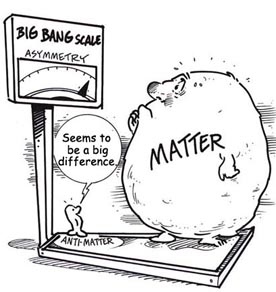
\includegraphics[height=0.5\textheight]{figs/matter-antimatter.jpg}
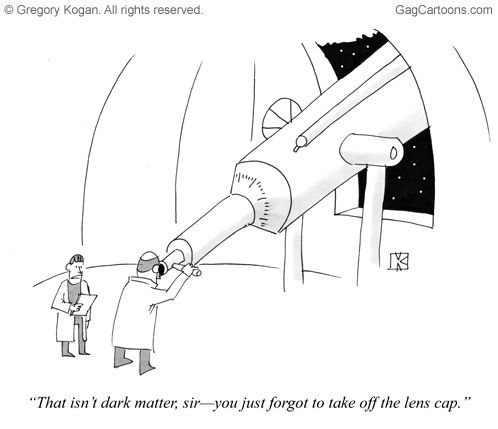
\includegraphics[height=0.5\textheight]{figs/darkmatter.jpg}
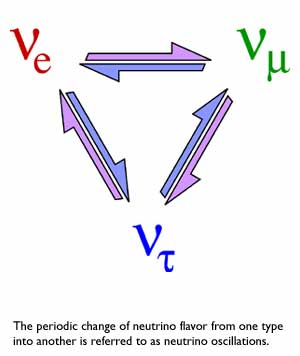
\includegraphics[height=0.5\textheight]{figs/13_oscill.jpeg}
\end{center}

\begin{itemize}
  \item[$\blacktriangleright$] The observed asymmetry between matter and antimatter in our Universe cannot be explained
  \item[$\blacktriangleright$] Dark matter, which is believed to be 5 times as abundant as ordinary matter, is not accounted for
  \item[$\blacktriangleright$] SM neutrinos are only left-handed and massless, but we know they have a small, non-zero mass
\end{itemize}
\end{frame}

%%%%%%%%%%%%%%%%%%%%%%%%%%%%%%%%%%%%%%%%%%%%%%%%%%%%%%%%%%%%%%%%%
%Slide
%%%%%%%%%%%%%%%%%%%%%%%%%%%%%%%%%%%%%%%%%%%%%%%%%%%%%%%%%%%%%%%%%
\begin{frame}{New Physics}
\begin{itemize}
\item[$\blacktriangleright$] These limitations have led particle physicists to look for extensions to the SM in the form of New Physics (NP) models
\end{itemize}

\begin{columns}
\begin{column}{0.5\textwidth}
\begin{itemize}
  \item[$\blacktriangleright$] e.g. Supersymmetry (SUSY)
\begin{itemize}
  \item[\ding{70}] Doubles the amount of particles
  \item[\ding{70}] Introduces fermionic partner to every boson and bosonic partner to every fermion
  \item[\ding{70}] Lightest supersymmetric particle provides dark matter candidate
\end{itemize}
\end{itemize}
\end{column}
\begin{column}{0.5\textwidth}
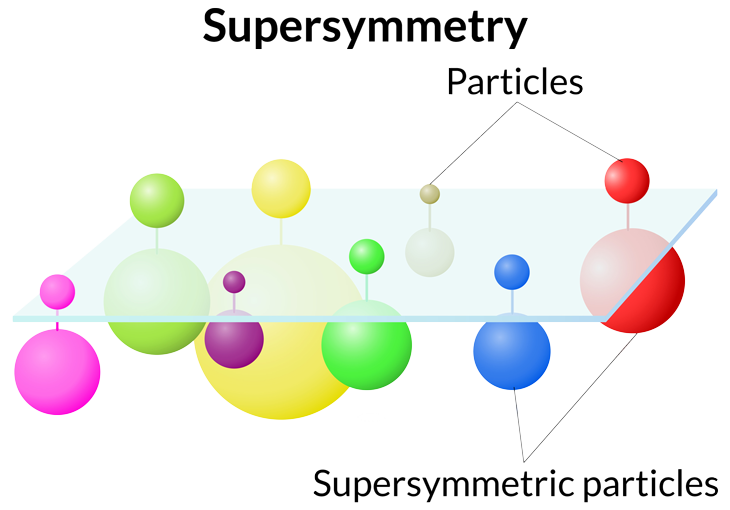
\includegraphics[width=\textwidth]{figs/supersymmetry.jpg}
\end{column}
\end{columns}

\bigskip

\begin{itemize}
\item[$\blacktriangleright$] Can search for these NP particles through {\bf direct} and {\bf indirect} approaches
   \begin{itemize}
     \item[\ding{70}] Direct \to produce new particles that can be directly detected
     \item[\ding{70}] Indirect \to study the effect of `virtual' particles within quantum loops
   \end{itemize}
\end{itemize}

\end{frame}

%%%%%%%%%%%%%%%%%%%%%%%%%%%%%%%%%%%%%%%%%%%%%%%%%%%%%%%%%%%%%%%%%
%Slide
%%%%%%%%%%%%%%%%%%%%%%%%%%%%%%%%%%%%%%%%%%%%%%%%%%%%%%%%%%%%%%%%%
% \begin{frame}{Direct searches for NP}

% \end{frame}

%%%%%%%%%%%%%%%%%%%%%%%%%%%%%%%%%%%%%%%%%%%%%%%%%%%%%%%%%%%%%%%%%
%Slide
%%%%%%%%%%%%%%%%%%%%%%%%%%%%%%%%%%%%%%%%%%%%%%%%%%%%%%%%%%%%%%%%%
\begin{frame}{Rare decays as indirect searches for NP}
\vspace{-0.2cm}
\begin{columns}
\begin{column}{0.5\textwidth}
\begin{myenv}{\color{bleudefrance}{SM}}[linecolor=bleudefrance]
\centering
\begin{tikzpicture}
\node[anchor=south west,inner sep=0](image) at (0,0) {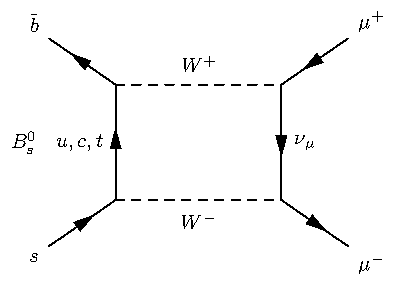
\includegraphics[width=0.9\textwidth]{figs/Bsmm-1.pdf}};
\begin{scope}[x={(image.south east)},y={(image.north west)}]
%\draw[help lines,xstep=.1,ystep=.1] (0,0) grid (1,1);
% \node[draw=none,bleudefrance] at (0.53,0.98) {\scriptsize \Wm};
% \node[draw=none,bleudefrance] at (0.3,0.6) {\scriptsize \tquark};
% \node[draw=none,bleudefrance] at (0.56,0.27) {\scriptsize {\small\Pgamma},$\Z^{0}$};
\end{scope}
\end{tikzpicture}
\end{myenv}
\end{column}
\begin{column}{0.5\textwidth}
\begin{myenv}{\color{bostonuniversityred}{NP}}[linecolor=bostonuniversityred]
\centering
\begin{tikzpicture}
\centering
\node[anchor=south west,inner sep=0](image) at (0,0) {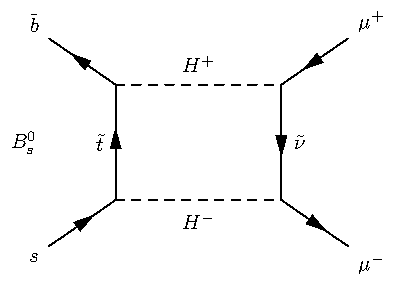
\includegraphics[width=0.9\textwidth]{figs/Bsmm-2.pdf}};
      \begin{scope}[x={(image.south east)},y={(image.north west)}]
      %\draw[help lines,xstep=.1,ystep=.1] (0,0) grid (1,1);
      % \node[draw=none,bostonuniversityred] at (0.5,0.96) {\small ?};
      % \node[draw=none,bostonuniversityred] at (0.3,0.6) {\small ?};
      % \node[draw=none,bostonuniversityred] at (0.58,0.27) {\small ?};
      \end{scope}
\end{tikzpicture}
\end{myenv}
\end{column}
\end{columns}

\bigskip

\begin{itemize}
\item[$\blacktriangleright$] Decays such as \Bsmm proceed via loop level processes
\item[$\blacktriangleright$] Virtual particles can ``borrow'' energy for a short time due to the Heisenberg uncertainty principle
\item[$\blacktriangleright$] In NP models, new particles would also appear in the loop
\item[$\blacktriangleright$] As decays such as \Bsmm are suppressed in the SM, NP can contribute at the same level and alter the properties of the decay in a measurable way
\end{itemize}

\end{frame}

%%%%%%%%%%%%%%%%%%%%%%%%%%%%%%%%%%%%%%%%%%%%%%%%%%%%%%%%%%%%%%%%%
%Slide
%%%%%%%%%%%%%%%%%%%%%%%%%%%%%%%%%%%%%%%%%%%%%%%%%%%%%%%%%%%%%%%%%
\begin{frame}{The \lhcb experiment}
  \begin{itemize}
  \item[$\blacktriangleright$] LHCb is a particle physics detector experiment located at the LHC 
  \item[$\blacktriangleright$] Its primary goal is to search for {\bf indirect} evidence of New Physics in the decays of \bquark and \cquark quarks
  \item[$\blacktriangleright$] Takes advantage of large production of \bquark\bquarkbar pairs in the \proton\proton collisions
  \end{itemize}

   \bigskip
    
   \begin{columns}
   \begin{column}{0.4\textwidth}
    \begin{itemize}
      \item[$\blacktriangleright$] Single arm forward spectrometer
      \item[$\blacktriangleright$] Excellent particle identification \mbox{(e.g. $\pi \to \mu <0.5\%$)}
      \item[$\blacktriangleright$] Excellent momentum resolution \mbox{(e.g. $\delta\ptot/\ptot \sim 0.5\%$)}
    \end{itemize}
    \end{column}
   \begin{column}{0.6\textwidth}
      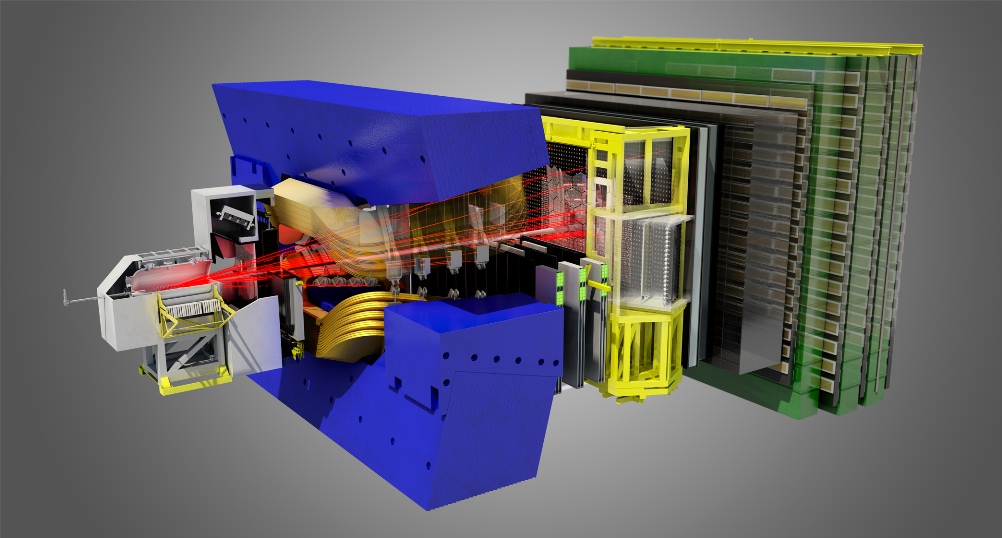
\includegraphics[width=\textwidth]{figs/lhcb/lhcb2.png}
    \end{column}
   \end{columns}
\end{frame}

%%%%%%%%%%%%%%%%%%%%%%%%%%%%%%%%%%%%%%%%%%%%%%%%%%%%%%%%%%%%%%%%%
%Slide
%%%%%%%%%%%%%%%%%%%%%%%%%%%%%%%%%%%%%%%%%%%%%%%%%%%%%%%%%%%%%%%%%
\begin{frame}\frametitle{}
  \begin{center}
    \begin{tikzpicture}
      \node[anchor=south west,inner sep=0](image) at (0,0) {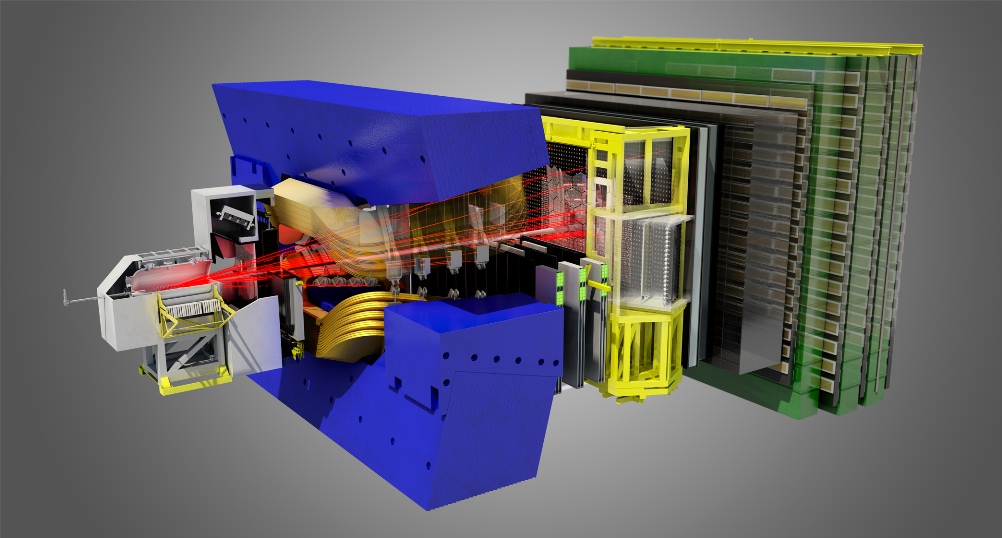
\includegraphics[width=\textwidth]{figs/lhcb/lhcb2.png}};
      
      \begin{scope}[x={(image.south east)},y={(image.north west)}]
        %\draw[help lines,xstep=.1,ystep=.1] (0,0) grid (1,1);
        
        \node[draw=none,burgundy] at (0.17,0.05) {Vertex Locator (\velo)};
        \draw[ultra thick,->,burgundy] (0.15,0.1) -- (0.2,0.4);
        
        \node[draw=none,cadmiumorange] at (0.20,0.95) {Tracking system (TT, IT, OT)};
        \draw[ultra thick,->,cadmiumorange] (0.14,0.9) -- (0.3,0.48);
        \draw[ultra thick,->,cadmiumorange] (0.14,0.9) -- (0.58,0.52); 
        
        \node[draw=none,byzantine] at (0.49,0.95) {RICH detectors};
        \draw[ultra thick,->,byzantine] (0.5,0.9) -- (0.23,0.55);
        \draw[ultra thick,->,byzantine] (0.5,0.9) -- (0.65,0.65);
        
        \node[draw=none,gray] at (0.45,0.2) {Magnet};
        
        \node[draw=none,babyblue] at (0.7,0.05) {Calorimeters};
        \draw[ultra thick,->,babyblue] (0.7,0.1) -- (0.75,0.55);
        
        \node[draw=none,green!90!black] at (0.9,0.7) {Muon system};
        
      \end{scope}
    \end{tikzpicture}
    
  \end{center}
\end{frame}

%%%%%%%%%%%%%%%%%%%%%%%%%%%%%%%%%%%%%%%%%%%%%%%%%%%%%%%%%%%%%%%%%
%Slide
%%%%%%%%%%%%%%%%%%%%%%%%%%%%%%%%%%%%%%%%%%%%%%%%%%%%%%%%%%%%%%%%%
\begin{frame}{Track reconstruction at \lhcb}

\begin{columns}
\begin{column}{0.5\textwidth}
\begin{itemize}
\item[$\blacktriangleright$] Track reconstruction is used to determine the trajectory and momentum of charged particles
\end{itemize}

\begin{itemize}
\item[$\blacktriangleright$] At \lhcb this is performed by several different software algorithms
\end{itemize}
\begin{itemize}
\item[$\blacktriangleright$] Two standalone algorithms 
  \begin{itemize}
    \item[\ding{70}] \velo tracking and T track seeding
  \end{itemize}
\item[$\blacktriangleright$] Other algorithms use input from these to perform further track reconstruction
  \begin{itemize}
    \item[\ding{70}] e.g. Forward tracking uses \velo tracks
  \end{itemize}
\end{itemize}

\begin{itemize}
  \item[$\blacktriangleright$] Upstream tracking refers to combining \velo tracks with TT hits
\end{itemize}

\end{column}
\begin{column}{0.5\textwidth}
\begin{tikzpicture}
\node[anchor=south west,inner sep=0](image) at (0,0) {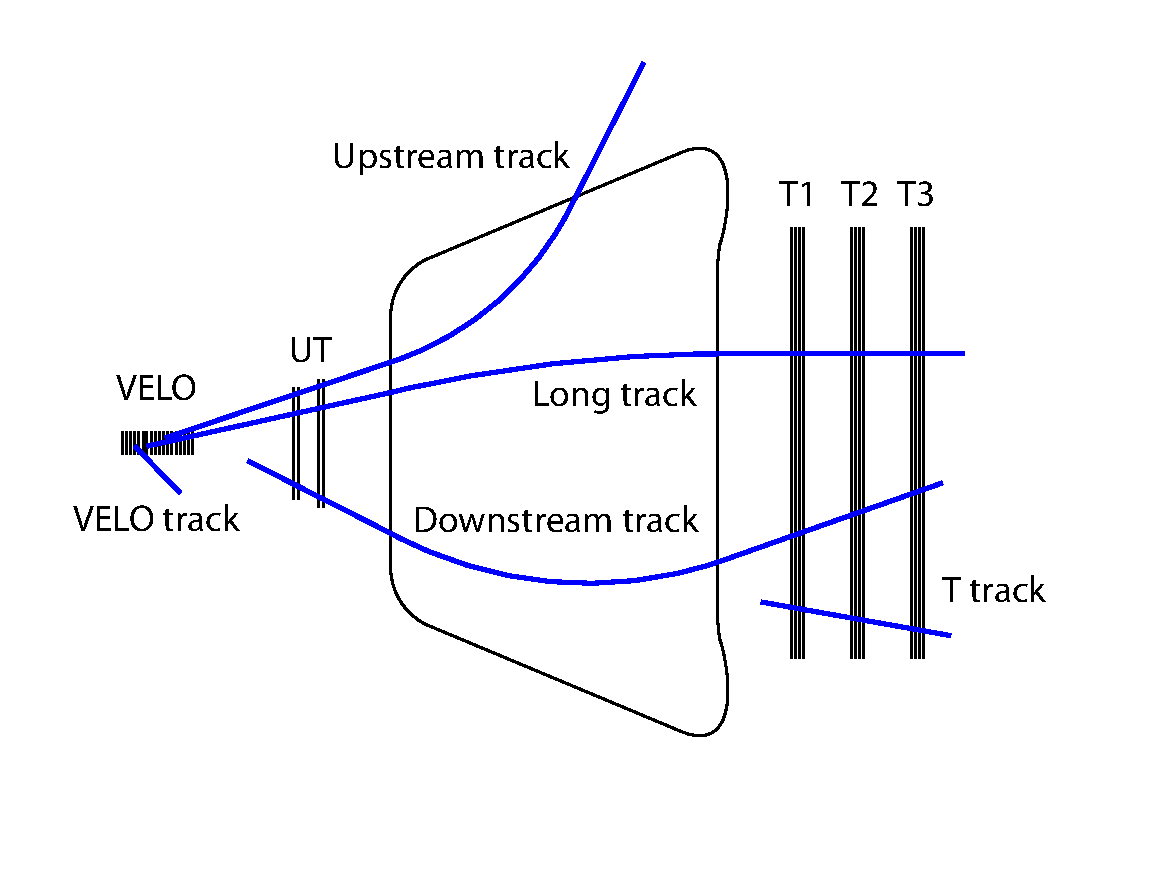
\includegraphics[trim={1cm 0 2cm 0},clip,width=\textwidth]{figs/tracking/trackTypes.pdf}};
\begin{scope}[x={(image.south east)},y={(image.north west)}]
%\draw[help lines,xstep=.1,ystep=.1] (0,0) grid (1,1);
\fill[white] (0.22,0.58) rectangle (0.29,0.62);
\node at (0.25,0.6) {\footnotesize {\fontfamily{cmss}\selectfont TT}};
\node at (0.55,0.1) {\footnotesize {\fontfamily{cmss}\selectfont Magnet}};
\end{scope}
\end{tikzpicture} 
\end{column}
\end{columns}
\end{frame}

%%%%%%%%%%%%%%%%%%%%%%%%%%%%%%%%%%%%%%%%%%%%%%%%%%%%%%%%%%%%%%%%%
%Slide
%%%%%%%%%%%%%%%%%%%%%%%%%%%%%%%%%%%%%%%%%%%%%%%%%%%%%%%%%%%%%%%%%
\begin{frame}{The \lhcb trigger in Run 1 (2010-2013)}

\begin{itemize}
  \item[$\blacktriangleright$] The data rate from every \proton\proton collision is too high to store information of every event
  \begin{itemize}
    \item[\ding{70}] 10 exobytes per year!
  \end{itemize}
  \item[$\blacktriangleright$] Moreover, many of the collisions are not of interest for physics analyses
  \item[$\blacktriangleright$] The \lhcb trigger plays an important role in selecting interesting events and reducing the data rate to disk 
\end{itemize}

\begin{itemize}
 \item[$\blacktriangleright$] During Run I, this consisted of two stages:
 \begin{itemize}
    \item[\ding{182}] Hardware trigger
    \begin{itemize}
      \item[\ding{70}] Decision based on information from muon system and calorimeters 
      \item[\ding{70}] Reduces data rate from $40\mhz\rightarrow1\mhz$
    \end{itemize}
    \item[\ding{183}] Software trigger 
    \begin{itemize}
      \item[\ding{70}] Track reconstruction performed
      \item[\ding{70}] Decision based on multivariate classifier
      \item[\ding{70}] Reduces data rate from 1\mhz $\rightarrow$ 5\khz, which is stored for offline analysis
    \end{itemize}
 \end{itemize}
\end{itemize}

\end{frame}

%%%%%%%%%%%%%%%%%%%%%%%%%%%%%%%%%%%%%%%%%%%%%%%%%%%%%%%%%%%%%%%%%
%Slide
%%%%%%%%%%%%%%%%%%%%%%%%%%%%%%%%%%%%%%%%%%%%%%%%%%%%%%%%%%%%%%%%%
\begin{frame}{The \lhcb Upgrade (2020+)}

\begin{columns}
\begin{column}{0.6\textwidth}
  \begin{itemize}
    \item[$\blacktriangleright$] \lhcb  will undergo an upgrade during 2018-2019 to allow data taking at higher energy and intensity
    \item[$\blacktriangleright$] Many existing subdetectors will be replaced
    \begin{itemize}
      \item[\ding{70}] e.g. TT replaced by UT
    \end{itemize}
  \end{itemize}

  \begin{itemize}
    \item[$\blacktriangleright$] Key feature: Full software trigger
    \begin{itemize}
      \item[\ding{70}] Remove hardware trigger stage
      \item[\ding{70}] Improved trigger efficiency for many physics channels
      \item[\ding{70}] Strict requirements placed on execution time of tracking algorithms
      \item[\ding{70}] Existing tracking sequence (\velo \to Forward) {\bf unable to meet timing budget!}
    \end{itemize}
    %     \item[\ding{70}] Read out full detector at 40\mhz
    %     \item[\ding{80}] Front end electronics need to be replaced
    %     \item[\ding{80}] Many existing sub-detectors will be upgraded
    %     %\begin{itemize}
    %     %  \item[\ding{80}] e.g. TT replaced by UT
    %     %\end{itemize}
    %   \end{itemize}
    % \begin{enumerate}
    %   \item Triggerless readout
    %   \begin{itemize}
    %     \item[\ding{70}] Remove hardware trigger 
    %     \item[\ding{70}] Read out full detector at 40\mhz
    %     \item[\ding{80}] Front end electronics need to be replaced
    %     \item[\ding{80}] Many existing sub-detectors will be upgraded
    %     %\begin{itemize}
    %     %  \item[\ding{80}] e.g. TT replaced by UT
    %     %\end{itemize}
    %   \end{itemize}
    %   \item Full software trigger
    %   \begin{itemize}
    %     \item[\ding{70}] Full event reconstruction
    %     \item[\ding{70}] Offers great flexibility for designing selections
    %     \item[\ding{70}] Increases trigger efficiency for many physics channels
    %     \item[\ding{80}] Strict requirements on execution time of tracking algorithms
    %     \item[\ding{80}] Existing tracking sequence {\bf unable to meet timing budget!}
    %   \end{itemize}
    % \end{enumerate}
  \end{itemize}

  % \begin{itemize}
  %   \item Front end electronics need to be replaced
  %   \item Many existing sub-detectors will be upgraded
  %   \begin{itemize}
  %       \item[\ding{70}] e.g. TT replaced by UT
  %     \end{itemize}
  % \end{itemize}

\end{column}
\begin{column}{0.4\textwidth}
\centering
\includegraphics[width=0.9\textwidth]{figs/detector/UT.pdf}\\~\\~\\
\begin{tikzpicture}
      \node[anchor=south west,inner sep=0](image) at (0,0) {
\includegraphics[width=0.9\textwidth]{figs/need-for-speed.png}};
      \begin{scope}[x={(image.south east)},y={(image.north west)}]
      %\draw[help lines,xstep=.1,ystep=.1] (0,0) grid (1,1);
      \node[draw=none] at (0.65,-0.1) {\bf LHCb Upgrade};
      %\node[draw=none,bleudefrance] at (0.3,0.6) {\scriptsize \tquark};
      %\node[draw=none,bleudefrance] at (0.56,0.27) {\scriptsize {\small\Pgamma},$\Z^{0}$};
      \end{scope}
      \end{tikzpicture}
%
\includegraphics[width=0.9\textwidth]{figs/need-for-speed.png}
\end{column}

\end{columns}

\end{frame}

% %%%%%%%%%%%%%%%%%%%%%%%%%%%%%%%%%%%%%%%%%%%%%%%%%%%%%%%%%%%%%%%%%
% %Slide
% %%%%%%%%%%%%%%%%%%%%%%%%%%%%%%%%%%%%%%%%%%%%%%%%%%%%%%%%%%%%%%%%%
% \begin{frame}{The \lhcb Upgrade (2020+)}

% \begin{columns}
% \begin{column}{0.6\textwidth}
%   \begin{itemize}
%     \item \lhcb  will undergo upgrade during 2018-2019 to allow data taking at \mbox{$\sqs=14\tev$ and $\lum=2\times10^{33}\cm^{-2}\sec^{-1}$}
%   \end{itemize}

%   \begin{itemize}
%     \item Two key features
%     \begin{enumerate}
%       \item Triggerless readout
%       \begin{itemize}
%         \item[\ding{70}] Remove L0 trigger bottleneck
%         \item[\ding{70}] Read out full detector at 40\mhz
%         \item[\ding{80}] Front end electronics need to be replaced
%         \item[\ding{80}] Many existing sub-detectors will be upgraded
%         %\begin{itemize}
%         %  \item[\ding{80}] e.g. TT replaced by UT
%         %\end{itemize}
%       \end{itemize}
%       \item Full software trigger
%       \begin{itemize}
%         \item[\ding{70}] Full event reconstruction
%         \item[\ding{70}] Offers great flexibility for designing selections
%         \item[\ding{70}] Increases trigger efficiency for many physics channels
%         \item[\ding{80}] Strict requirements on execution time of tracking algorithms
%         \item[\ding{80}] Existing tracking sequence {\bf unable to meet timing budget!}
%       \end{itemize}
%     \end{enumerate}
%   \end{itemize}

%   % \begin{itemize}
%   %   \item Front end electronics need to be replaced
%   %   \item Many existing sub-detectors will be upgraded
%   %   \begin{itemize}
%   %       \item[\ding{70}] e.g. TT replaced by UT
%   %     \end{itemize}
%   % \end{itemize}

% \end{column}
% \begin{column}{0.4\textwidth}
% \centering
% \vspace{-1cm}
% \adjincludegraphics[width=\textwidth,trim={{.3\width} {.575\height} {.28\width} {.1\height}},clip]{figs/detector/upgrade-motivation.pdf}
% \includegraphics[width=0.8\textwidth]{figs/detector/UT.pdf}
% \end{column}

% \end{columns}

% \end{frame}

%%%%%%%%%%%%%%%%%%%%%%%%%%%%%%%%%%%%%%%%%%%%%%%%%%%%%%%%%%%%%%%%%
%Slide
%%%%%%%%%%%%%%%%%%%%%%%%%%%%%%%%%%%%%%%%%%%%%%%%%%%%%%%%%%%%%%%%%
\begin{frame}{Novel idea}
\begin{itemize}
  \item[$\blacktriangleright$] Can using upstream tracks speed up the full tracking sequence? \mbox{(\velo $\to$ [Upstream] $\to$ Forward)}
\end{itemize}
\begin{itemize}
  \item[$\blacktriangleright$] Advantages of using upstream (VeloUT) tracks over just VELO tracks
    \begin{itemize}
      \item[\ding{70}] Charge and momentum of track segment ($\delta \ptot/\ptot \sim 15 \%$)
      \begin{itemize}
        \item[\ding{70}] Preselect on track \pt
        \item[\ding{70}] Open smaller search windows
        %\item[\ding{70}] Greatly reduce execution time and ghost rate!
        \item[\ding{70}] Greatly reduce execution time!
      \end{itemize}
    \end{itemize}
  \end{itemize}

  \begin{center}
  \resizebox{0.8\columnwidth}{!}{
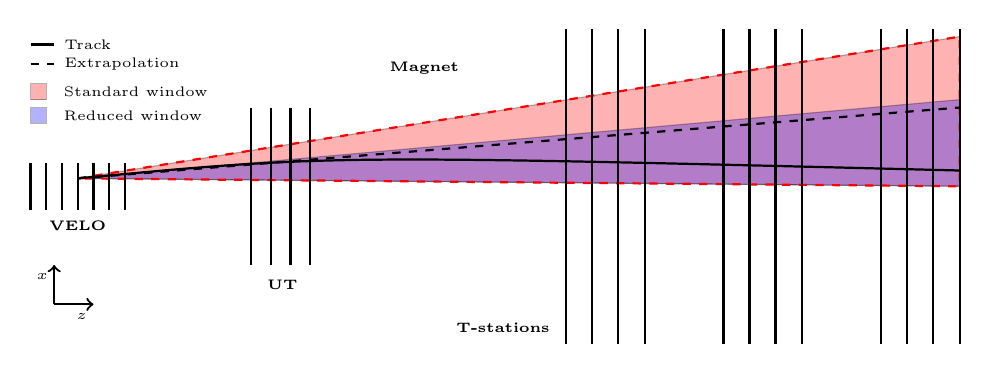
\begin{tikzpicture}
  %\draw[step=1cm,gray,very thin] (0,0) grid (12,4);

  \draw[fill=red,opacity=0.3] (0.8,2.1) -- (12.0,3.9) -- (12.0,2.0)--cycle;
  \draw[fill=blue,opacity=0.3] (0.8,2.1) -- (12.0,3.1) -- (12.0,2.0)--cycle;
  \draw[color=red,dashed,thick] (0.8,2.1) -- (12.0,3.9) -- (12.0,2.0)--cycle;

  %VELO
  \node[draw=none] at  (0.8,1.5){\tiny \bf{VELO}};
  \draw[thick] (0.2,1.7) -- (0.2,2.3);
  \draw[thick] (0.4,1.7) -- (0.4,2.3);
  \draw[thick] (0.6,1.7) -- (0.6,2.3);
  \draw[thick] (0.8,1.7) -- (0.8,2.3);
  \draw[thick] (1.0,1.7) -- (1.0,2.3);
  \draw[thick] (1.2,1.7) -- (1.2,2.3);
  \draw[thick] (1.4,1.7) -- (1.4,2.3);

  %TT
  \node[draw=none] at  (3.4,0.75){\tiny \bf{UT}};
  \draw[thick] (3.0,1.0) -- (3.0,3.0);
  \draw[thick] (3.25,1.0) -- (3.25,3.0);
  \draw[thick] (3.5,1.0) -- (3.5,3.0);
  \draw[thick] (3.75,1.0) -- (3.75,3.0);

  %T
  \node[draw=none] at  (6.2,0.2){\tiny \bf{T-stations}};
  \draw[thick] (7.0,0.0) -- (7.0,4.0);
  \draw[thick] (7.33,0.0) -- (7.33,4.0);
  \draw[thick] (7.66,0.0) -- (7.66,4.0);
  \draw[thick] (8.0,0.0) -- (8.0,4.0);

  \draw[thick] (9.0,0.0) -- (9.0,4.0);
  \draw[thick] (9.33,0.0) -- (9.33,4.0);
  \draw[thick] (9.66,0.0) -- (9.66,4.0);
  \draw[thick] (10.0,0.0) -- (10.0,4.0);

  \draw[thick] (11.0,0.0) -- (11.0,4.0);
  \draw[thick] (11.33,0.0) -- (11.33,4.0);
  \draw[thick] (11.66,0.0) -- (11.66,4.0);
  \draw[thick] (12.0,0.0) -- (12.0,4.0);

  \draw[thick,dashed] (0.8,2.1) -- (12,2+10*0.1);
  \draw[thick] (0.8,2.1) .. controls (4,2.4) .. (12,2.2);

  \draw[thick] (0.2,3.8) -- (0.5,3.8)  node[anchor=west] {\tiny Track};
  \draw[thick,dashed] (0.2,3.55) -- (0.5,3.55)  node[anchor=west] {\tiny Extrapolation};
  \draw[white] (0.2,3.2) -- (0.5,3.2)  node[anchor=west] {\tiny \textcolor{black}{Standard window}};
  \draw[white] (0.2,2.9) -- (0.5,2.9)  node[anchor=west] {\tiny \textcolor{black}{Reduced window}};
  \draw[fill=red,opacity=0.3] (0.2,3.1) rectangle (0.4,3.3);
  \draw[fill=blue,opacity=0.3] (0.2,2.8) rectangle (0.4,3.0);
  %\node[draw=none] at  (1.5,3.2){\tiny Standard window};
  %\node[draw=none] at  (1.5,2.9){\tiny Reduced window};

  \draw[thick,->] (0.5,0.5) -- (0.5,1.0);
  \draw[thick,->] (0.5,0.5) -- (1.0,0.5);
  \node[draw=none] at (0.35,0.85){\tiny $x$};
  \node[draw=none] at (0.85,0.35){\tiny $z$};

  \node[draw=none] at  (5.2,3.5){\tiny \bf{Magnet}};

\end{tikzpicture}
}

  \end{center}

  \begin{itemize}
    \item[$\blacktriangleright$] Upstream tracking algorithm needs to be both fast and efficient
  \end{itemize}
\end{frame}

%%%%%%%%%%%%%%%%%%%%%%%%%%%%%%%%%%%%%%%%%%%%%%%%%%%%%%%%%%%%%%%%%
%Slide
%%%%%%%%%%%%%%%%%%%%%%%%%%%%%%%%%%%%%%%%%%%%%%%%%%%%%%%%%%%%%%%%%
\begin{frame}\frametitle{Upstream tracking (VeloTT) in Run 1}
  \begin{itemize}
  \item[$\blacktriangleright$] Linearly extrapolate VELO track to TT
  \item[$\blacktriangleright$] Open search windows in each layer: calculate $\Delta x$ between track and hits
  \item[$\blacktriangleright$] Scale $\Delta x$ to reference plane at center of TT
  \item[$\blacktriangleright$] Choose clusters of hits consistent with coming from the same VELO track
  \begin{itemize}
    \item[\ding{70}] Each hit must be on the same side of the linear extrapolation
  \end{itemize}
  \item[$\blacktriangleright$] Fit each track candidate with a simple $\chi^{2}$ fit
  %\item[$\blacktriangleright$] Choose best candidate track based on \mbox{\# layers} fired and $\chi^{2}$
  \item[$\blacktriangleright$] Fit track with a Kalman filter (slow)
  \end{itemize}
  \resizebox{\columnwidth}{!}{
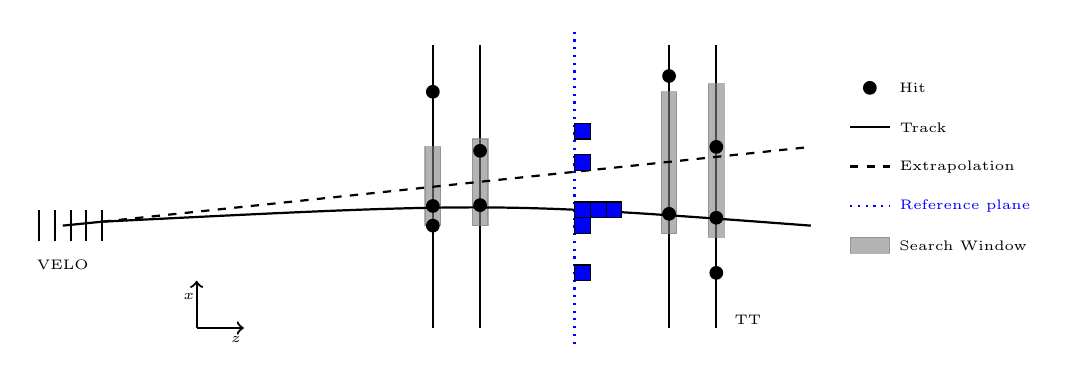
\begin{tikzpicture}
  %\draw[step=1cm,gray,very thin] (0,0) grid (13,4);

  \draw[thick,->] (2.2,0.2) -- (2.2,0.8);
  \draw[thick,->] (2.2,0.2) -- (2.8,0.2);
  \node[draw=none] at (2.1,0.6){\tiny $x$};
  \node[draw=none] at (2.7,0.05){\tiny $z$};

  \draw[thick] (0.2,1.3) -- (0.2,1.7);
  \draw[thick] (0.4,1.3) -- (0.4,1.7);
  \draw[thick] (0.6,1.3) -- (0.6,1.7);
  \draw[thick] (0.8,1.3) -- (0.8,1.7);
  \draw[thick] (1.0,1.3) -- (1,1.7);

  \draw[thick] (5.2,0.2) -- (5.2,3.8);
  \draw[thick] (5.8,0.2) -- (5.8,3.8);
  \draw[thick] (8.2,0.2) -- (8.2,3.8);
  \draw[thick] (8.8,0.2) -- (8.8,3.8);

  \draw[thick,dotted,blue] (7,0) -- (7,4);

  \draw[fill,gray,opacity=0.6] (5.1,1.5) rectangle (5.3,2.5);
  \draw[fill,gray,opacity=0.6] (5.7,1.5) rectangle (5.9,2.6);
  \draw[fill,gray,opacity=0.6] (8.1,1.4) rectangle (8.3,3.2);
  \draw[fill,gray,opacity=0.6] (8.7,1.35) rectangle (8.9,3.3);
  
  \draw[thick] (0.5,1.5) -- (1,1.5+0.5*0.1);
  \draw[thick,dashed] (1,1.5+0.5*0.1) -- (10,1.5+10*0.1);
  \draw[thick] (1,1.5+0.5*0.1) .. controls (6,1.8) .. (10,1.5);

  \draw[fill] (5.2,1.75) circle (0.08);
  \draw[fill] (5.8,1.76) circle (0.08);
  \draw[fill] (8.2,1.65) circle (0.08);
  \draw[fill] (8.8,1.6) circle (0.08);

  \draw[fill] (5.2,1.5) circle (0.08);
  \draw[fill] (5.2,3.2) circle (0.08);
  \draw[fill] (5.8,2.45) circle (0.08);
  \draw[fill] (8.2,3.4) circle (0.08);
  \draw[fill] (8.8,2.5) circle (0.08);
  \draw[fill] (8.8,0.9) circle (0.08);

  \fill[blue,draw=black] (7.0,1.6) rectangle (7.2,1.8);
  \fill[blue,draw=black] (7.2,1.6) rectangle (7.4,1.8);
  \fill[blue,draw=black] (7.4,1.6) rectangle (7.6,1.8);
  \fill[blue,draw=black] (7.0,1.4) rectangle (7.2,1.6);

  \fill[blue,draw=black] (7.0,0.8) rectangle (7.2,1.);
  \fill[blue,draw=black] (7.0,2.2) rectangle (7.2,2.4);
  \fill[blue,draw=black] (7.0,2.6) rectangle (7.2,2.8);

  \node[draw=none] at (0.5,1){\tiny VELO};
  \node[draw=none] at (9.2,0.3){\tiny TT};

  %\draw[thick] (10.5,3.25) -- (11.,3.25)  node[anchor=west] {\tiny Track};
  %\draw[fill] (11.,3.25) circle [radius=2pt]  node[anchor=west] {\tiny Hit};
  \draw[white] (10.5,3.25) -- (11.,3.25)  node[anchor=west] {\tiny \textcolor{black}{Hit}};
  \draw[fill] (10.75,3.25) circle (0.08);
  \draw[thick] (10.5,2.75) -- (11.,2.75)  node[anchor=west] {\tiny Track};
  \draw[thick,dashed] (10.5,2.25) -- (11.,2.25)  node[anchor=west] {\tiny Extrapolation};
  \draw[thick,dotted,blue] (10.5,1.75) -- (11.,1.75)  node[anchor=west] {\tiny Reference plane};
  \draw[white] (10.5,1.25) -- (11.,1.25)  node[anchor=west] {\tiny \textcolor{black}{Search Window}};
  \draw[fill,gray,opacity=0.6] (10.5,1.15) rectangle (11.0,1.35);
  %\node[draw=none] at (12.0,1.25){\tiny };
\end{tikzpicture}
}

\end{frame}

%%%%%%%%%%%%%%%%%%%%%%%%%%%%%%%%%%%%%%%%%%%%%%%%%%%%%%%%%%%%%%%%%
%Slide
%%%%%%%%%%%%%%%%%%%%%%%%%%%%%%%%%%%%%%%%%%%%%%%%%%%%%%%%%%%%%%%%%
\begin{frame}{Track reconstruction: Performance}

\begin{itemize}
  \item[$\blacktriangleright$] Three important figures of merit used to evaluate the performance of tracking algorithms
\end{itemize}
\begin{itemize}
  \item[\ding{182}] Reconstruction efficiency
  \begin{itemize}
    \item[\ding{70}] N(reconstructible \& reconstructed)/N(reconstructible)
    \item[\ding{70}] Reconstructible means having left sufficient hits in the tracking stations
    \item[\ding{70}] Determined using simulation
  \end{itemize}
\end{itemize}
\begin{itemize}
  \item[\ding{183}] Ghost rate
  \begin{itemize}
  \item[\ding{70}] N(ghost tracks)/N(tracks)
  \item[\ding{70}] A ghost track is one which has no matching simulated particle
  \item[\ding{70}] Determined using simulation
  \end{itemize}
\end{itemize}
\begin{itemize}
  \item[\ding{184}] Average execution time per event
\end{itemize}

\end{frame}
%%%%%%%%%%%%%%%%%%%%%%%%%%%%%%%%%%%%%%%%%%%%%%%%%%%%%%%%%%%%%%%%%
%Slide
%%%%%%%%%%%%%%%%%%%%%%%%%%%%%%%%%%%%%%%%%%%%%%%%%%%%%%%%%%%%%%%%%
\begin{frame}{VeloUT: Initial performance}

\begin{columns}
\begin{column}{0.65\textwidth}

\begin{itemize}
  \item[$\blacktriangleright$] Initial version of VeloUT was a replication of the VeloTT algorithm from Run 1
\end{itemize}

\begin{itemize}
  \item[$\blacktriangleright$] Execution time of 27.20\ms is {\bf far too slow} to use in the software trigger
  \begin{itemize}
    \item[\ding{70}] c.f. VELO tracking $\sim1.8\ms$
  \end{itemize}
  \item[$\blacktriangleright$] Reconstruction efficiency is {\bf too low}
  \begin{itemize}
    \item[\ding{70}] Any inefficiency will be propagated to next step
    \item[\ding{70}] Decreases as a function of momentum
  \end{itemize}
\end{itemize}

\bigskip

\begin{mdframed}[linecolor=barcolor]
\begin{center}
\resizebox{\columnwidth}{!}{
\begin{tabular}{c|c|c|c}
  \velout & Efficiency [\%] & Ghost rate [\%] & Timing [ms] \\ 
  \hline
  v1r2  & 93.94  & 7.21  &  27.20  \\
 \end{tabular}
 }
\end{center}
\end{mdframed}
\end{column}

\begin{column}{0.35\textwidth}
\centering
\begin{figure}
\vspace*{-1cm}
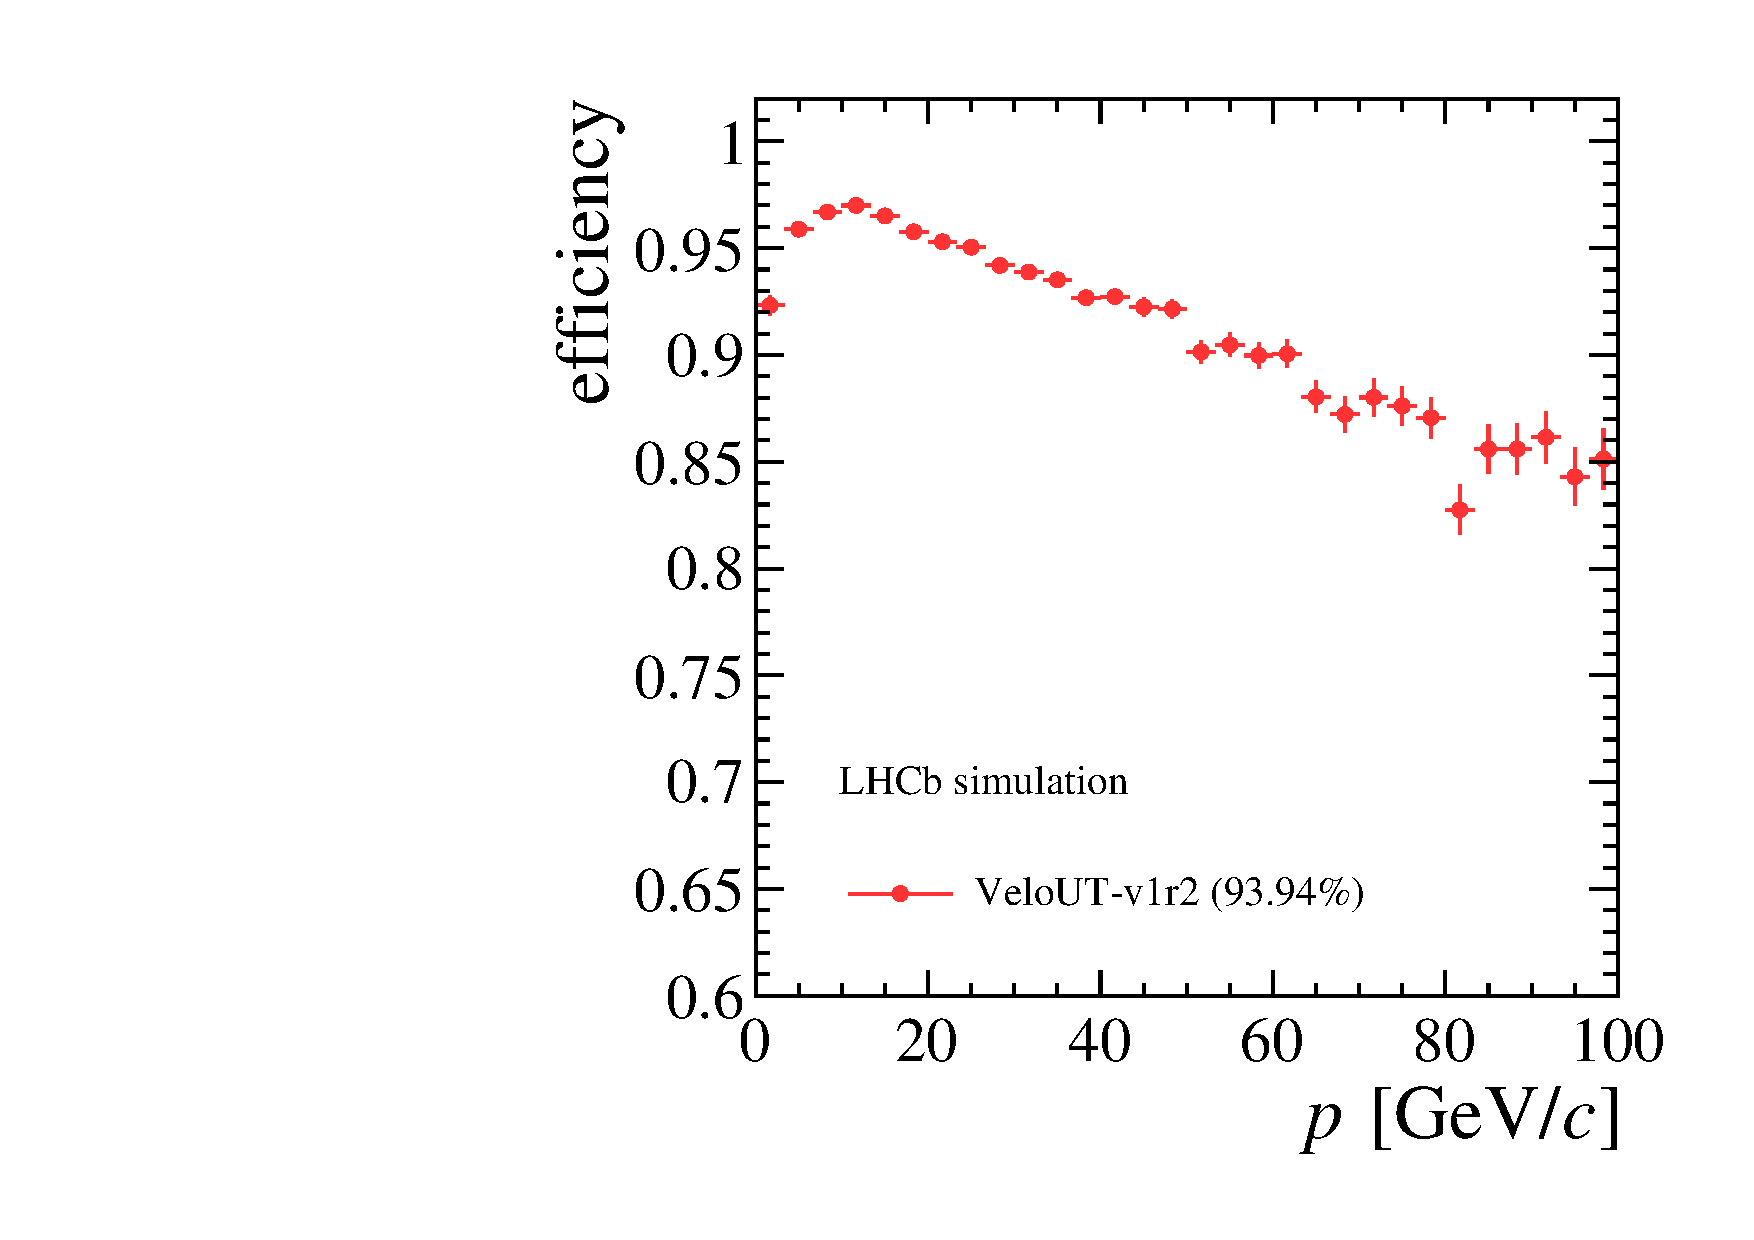
\includegraphics[height=0.475\textheight]{figs/upstream-tracking-upgrade/eff_p_v1r2.pdf}\\
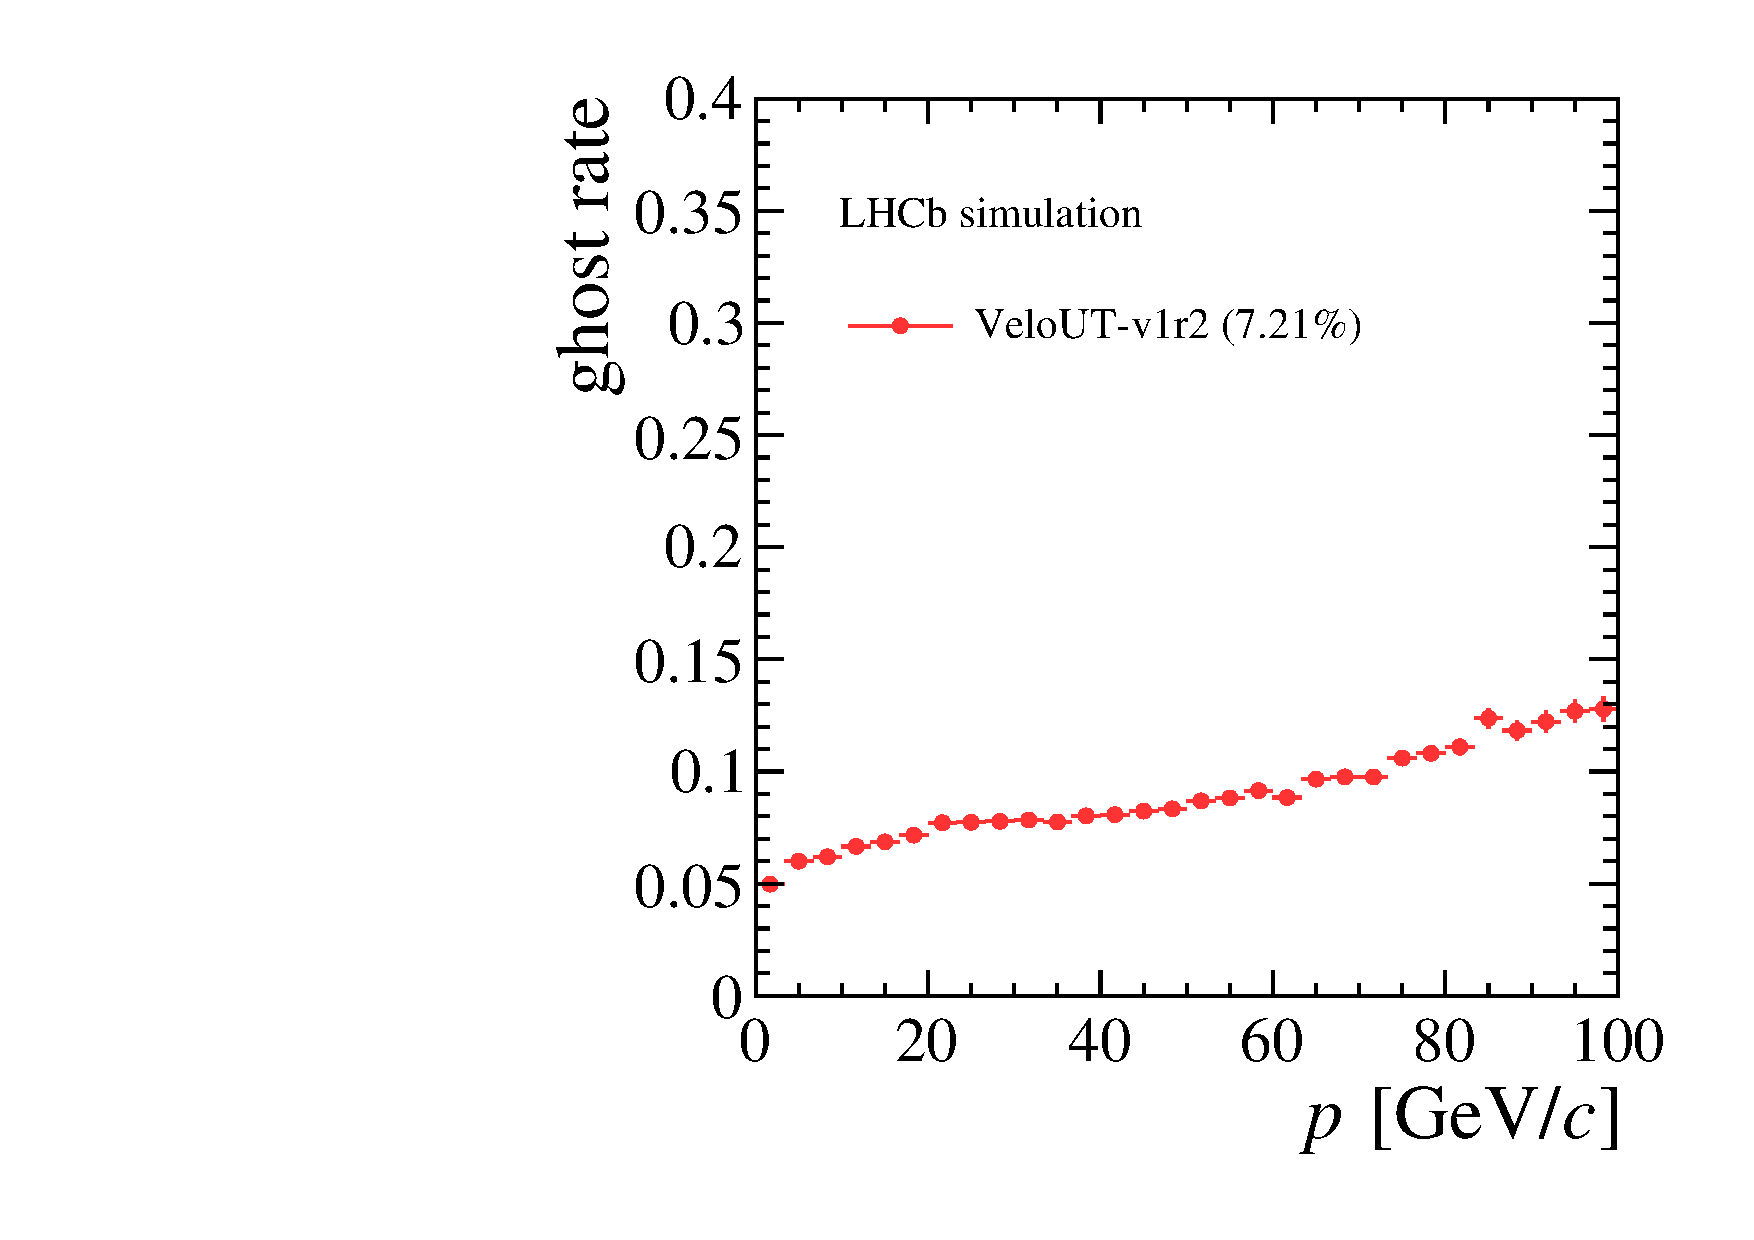
\includegraphics[height=0.475\textheight]{figs/upstream-tracking-upgrade/gr_p_v1r2.pdf}
\end{figure}
\end{column}
\end{columns}

\end{frame}

%%%%%%%%%%%%%%%%%%%%%%%%%%%%%%%%%%%%%%%%%%%%%%%%%%%%%%%%%%%%%%%%%
%Slide
%%%%%%%%%%%%%%%%%%%%%%%%%%%%%%%%%%%%%%%%%%%%%%%%%%%%%%%%%%%%%%%%%
\begin{frame}{VeloUT: Improvements}

\begin{myenv}{Execution time much too slow for use in trigger}[linecolor=barcolor]
  \begin{itemize}
    \setlength{\itemindent}{0.5em}
    \item[$\blacktriangleright$] Introduced hit sorting and binary searches
    \item[$\blacktriangleright$] Removed Kalman filter, simple $\chi^{2}$ fit is sufficient
    \item[$\blacktriangleright$] Numerous \cpp optimisations/changes to the logic
  \end{itemize}
\end{myenv}

\begin{myenv}{Efficiency too low/decreasing with increasing momentum}[linecolor=barcolor]
  \begin{itemize}
    \setlength{\itemindent}{0.5em}
    \item[$\blacktriangleright$] Tracked down to poor assumptions made when associating hits to \velo tracks
    \item[$\blacktriangleright$] Developed new hit clustering sequence 
  \end{itemize}
\end{myenv}

\end{frame}

%%%%%%%%%%%%%%%%%%%%%%%%%%%%%%%%%%%%%%%%%%%%%%%%%%%%%%%%%%%%%%%%%
%Slide
%%%%%%%%%%%%%%%%%%%%%%%%%%%%%%%%%%%%%%%%%%%%%%%%%%%%%%%%%%%%%%%%%
\begin{frame}{VeloUT: Optimised algorithm}
\begin{columns}
\begin{column}{0.5\textwidth}
\begin{itemize}
  \item[$\blacktriangleright$] Linearly extrapolate VELO track to UT
  \item[$\blacktriangleright$] Select hits within a search window around the extrapolated track
  \item[\ding{72}] Form doublets of hits in the first two layers
  \item[\ding{72}] Extrapolate doublets to third/fourth layers and search for compatible hits
  %\item[\ding{80}] If no four hit candidates found, repeat starting from last two layers
  \item[$\blacktriangleright$] Fit each track candidate with a simple $\chi^{2}$ fit% and estimate $q/p$ ($\delta p/p \sim 15 \%$)
  %\item[$\blacktriangleright$] Choose best candidate track based on \mbox{\# layers} fired and $\chi^{2}$
  \end{itemize}
\end{column}
\begin{column}{0.5\textwidth}
\centering
\resizebox{0.8\textheight}{!}{
  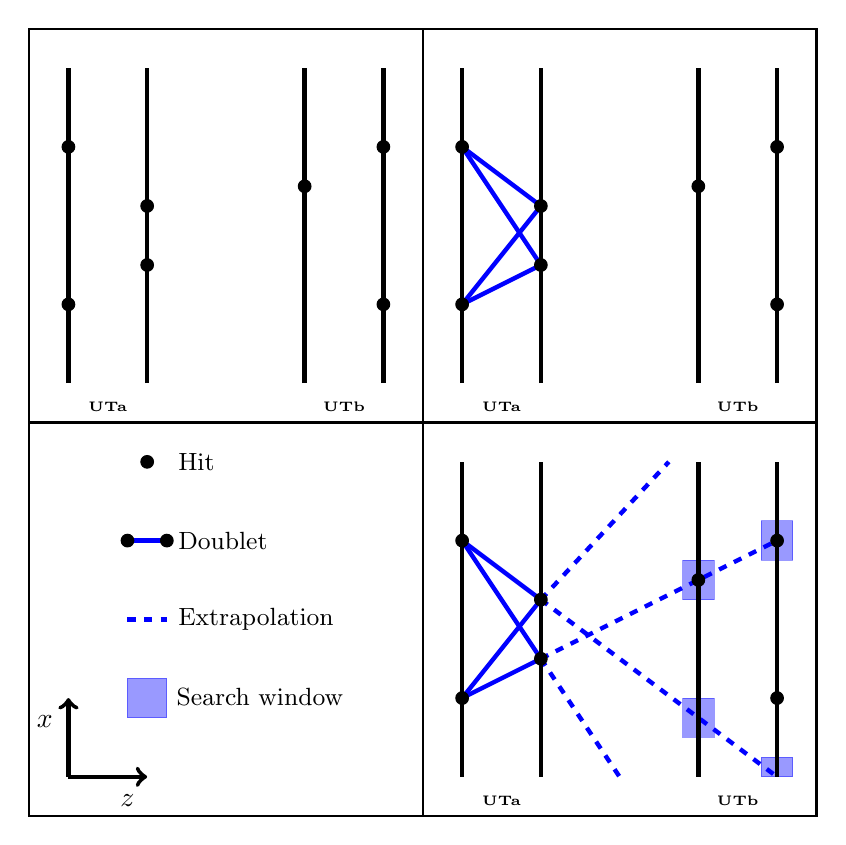
\begin{tikzpicture}
  %\draw[step=1cm,gray,very thin] (0,0) grid (10,10);

  %layout
  \draw[thick] (0,0) rectangle (5,5);
  \draw[thick] (5,0) rectangle (10,5);
  \draw[thick] (0,5) rectangle (5,10);
  \draw[thick] (5,5) rectangle (10,10);

  \draw[thick] (5.0,0.0) -- (5.0,10.0);
  \draw[thick] (0.0,5.0) -- (10.0,5.0);

  %first diagram
  %UT layers
  \draw[ultra thick] (0.5,5.5) -- (0.5,9.5);
  \draw[ultra thick] (1.5,5.5) -- (1.5,9.5);
  \draw[ultra thick] (3.5,5.5) -- (3.5,9.5);
  \draw[ultra thick] (4.5,5.5) -- (4.5,9.5);

  %true hits
  \draw[fill] (0.5,6.5) circle (0.08);
  \draw[fill] (1.5,7.0) circle (0.08);
  \draw[fill] (3.5,8.0) circle (0.08);
  \draw[fill] (4.5,8.5) circle (0.08);

  %fake hits
  \draw[fill] (0.5,8.5) circle (0.08);
  \draw[fill] (1.5,7.75) circle (0.08);
  \draw[fill] (4.5,6.5) circle (0.08);

  %labels
  \node[draw=none] at  (1,5.2){\tiny \bf{UTa}};
  \node[draw=none] at  (4,5.2){\tiny \bf{UTb}};

  %second diagram
  %doublets
  \draw[ultra thick,blue] (5.5,6.5) -- (6.5,7);
  \draw[ultra thick,blue] (5.5,6.5) -- (6.5,7.75);

  \draw[ultra thick,blue] (5.5,8.5) -- (6.5,7);
  \draw[ultra thick,blue] (5.5,8.5) -- (6.5,7.75);

  %UT layers
  \draw[ultra thick] (5.5,5.5) -- (5.5,9.5);
  \draw[ultra thick] (6.5,5.5) -- (6.5,9.5);
  \draw[ultra thick] (8.5,5.5) -- (8.5,9.5);
  \draw[ultra thick] (9.5,5.5) -- (9.5,9.5);

  %true hits
  \draw[fill] (5.5,6.5) circle (0.08);
  \draw[fill] (6.5,7.0) circle (0.08);
  \draw[fill] (8.5,8.0) circle (0.08);
  \draw[fill] (9.5,8.5) circle (0.08);

  %fake hits
  \draw[fill] (5.5,8.5) circle (0.08);
  \draw[fill] (6.5,7.75) circle (0.08);
  \draw[fill] (9.5,6.5) circle (0.08);

  %labels
  \node[draw=none] at  (6,5.2){\tiny \bf{UTa}};
  \node[draw=none] at  (9,5.2){\tiny \bf{UTb}};

  %third diagram
  %doublets
  \draw[ultra thick,blue] (5.5,1.5) -- (6.5,2.0);
  \draw[ultra thick,blue] (5.5,1.5) -- (6.5,2.75);

  \draw[ultra thick,blue] (5.5,3.5) -- (6.5,2.0);
  \draw[ultra thick,blue] (5.5,3.5) -- (6.5,2.75);

  %extrapolations
  %true
  \draw[ultra thick,blue,dashed] (6.5,2.0) -- (9.5,3.5);
  %fake
  \draw[ultra thick,blue,dashed] (6.5,2.0) -- (7.5,0.5);
  \draw[ultra thick,blue,dashed] (6.5,2.75) -- (8.125,4.5);
  \draw[ultra thick,blue,dashed] (6.5,2.75) -- (9.5,0.5);

  %search windows
  %true
  \draw[fill,blue,opacity=0.4] (8.3,2.75) rectangle (8.7,3.25);
  \draw[fill,blue,opacity=0.4] (9.3,3.25) rectangle (9.7,3.75);
  %fake
  \draw[fill,blue,opacity=0.4] (8.3,1.0) rectangle (8.7,1.50);
  \draw[fill,blue,opacity=0.4] (9.3,0.5) rectangle (9.7,0.75);

  %UT layers
  \draw[ultra thick] (5.5,0.5) -- (5.5,4.5);
  \draw[ultra thick] (6.5,0.5) -- (6.5,4.5);
  \draw[ultra thick] (8.5,0.5) -- (8.5,4.5);
  \draw[ultra thick] (9.5,0.5) -- (9.5,4.5);

  %true hits
  \draw[fill] (5.5,1.5) circle (0.08);
  \draw[fill] (6.5,2.0) circle (0.08);
  \draw[fill] (8.5,3.0) circle (0.08);
  \draw[fill] (9.5,3.5) circle (0.08);

  %fake hits
  \draw[fill] (5.5,3.5) circle (0.08);
  \draw[fill] (6.5,2.75) circle (0.08);
  \draw[fill] (9.5,1.5) circle (0.08);

  %labels
  \node[draw=none] at  (6,0.2){\tiny \bf{UTa}};
  \node[draw=none] at  (9,0.2){\tiny \bf{UTb}};

  %legend
  \draw[ultra thick, white] (1.25,4.5) -- (1.75,4.5)  node[anchor=west] {\small \textcolor{black}{Hit}};
  \draw[fill] (1.5,4.5) circle (0.08);

  \draw[ultra thick, blue] (1.25,3.5) -- (1.75,3.5)  node[anchor=west] {\small \textcolor{black}{Doublet}};
  \draw[fill] (1.25,3.5) circle (0.08);
  \draw[fill] (1.75,3.5) circle (0.08);

  \draw[ultra thick, blue,dashed] (1.25,2.5) -- (1.75,2.5) node[anchor=west] {\small \textcolor{black}{Extrapolation}};

  \draw[fill,blue,opacity=0.4,text opacity=1] (1.25,1.25) rectangle (1.75,1.75) node[anchor=north west] {\small \textcolor{black}{Search window}};

  \draw[ultra thick,->] (0.5,0.5) -- (0.5,1.5);
  \draw[ultra thick,->] (0.5,0.5) -- (1.5,0.5);
  \node[draw=none] at  (1.25,0.2){$z$};
  \node[draw=none] at  (0.2,1.2){$x$};

  \end{tikzpicture}
}
   
\end{column}
\end{columns}
\end{frame}

%%%%%%%%%%%%%%%%%%%%%%%%%%%%%%%%%%%%%%%%%%%%%%%%%%%%%%%%%%%%%%%%%
%Slide
%%%%%%%%%%%%%%%%%%%%%%%%%%%%%%%%%%%%%%%%%%%%%%%%%%%%%%%%%%%%%%%%%
\begin{frame}{VeloUT: Optimised peformance}

\begin{columns}
\begin{column}{0.65\textwidth}
\begin{itemize}
  \item[$\blacktriangleright$] Huge reduction in the execution time ($\times$33!)
  \item[$\blacktriangleright$] Large improvement in the efficiency ($+5$\%)
  \begin{itemize}
    \item[\ding{70}] Now flat in \ptot
  \end{itemize}
  \item[$\blacktriangleright$] Slight increase in the ghost rate ($+0.8$\%)
  \begin{itemize}
    \item[\ding{70}] Can be reduced in offline analysis
  \end{itemize}
\end{itemize}

\bigskip

\begin{mdframed}[linecolor=barcolor]
\begin{center}
\resizebox{\columnwidth}{!}{
\begin{tabular}{c|c|c|c}
  \velout & Efficiency [\%] & Ghost rate [\%] & Timing [ms] \\ 
  \hline
  v1r2  & 93.94  & 7.21  &  27.20  \\
  v2r2  & 98.69  & 8.00 &  \hphantom{0}0.81  \\
 \end{tabular}
 }
\end{center}
\end{mdframed}
\end{column}

\begin{column}{0.35\textwidth}
\centering
\begin{figure}
\vspace*{-1cm}
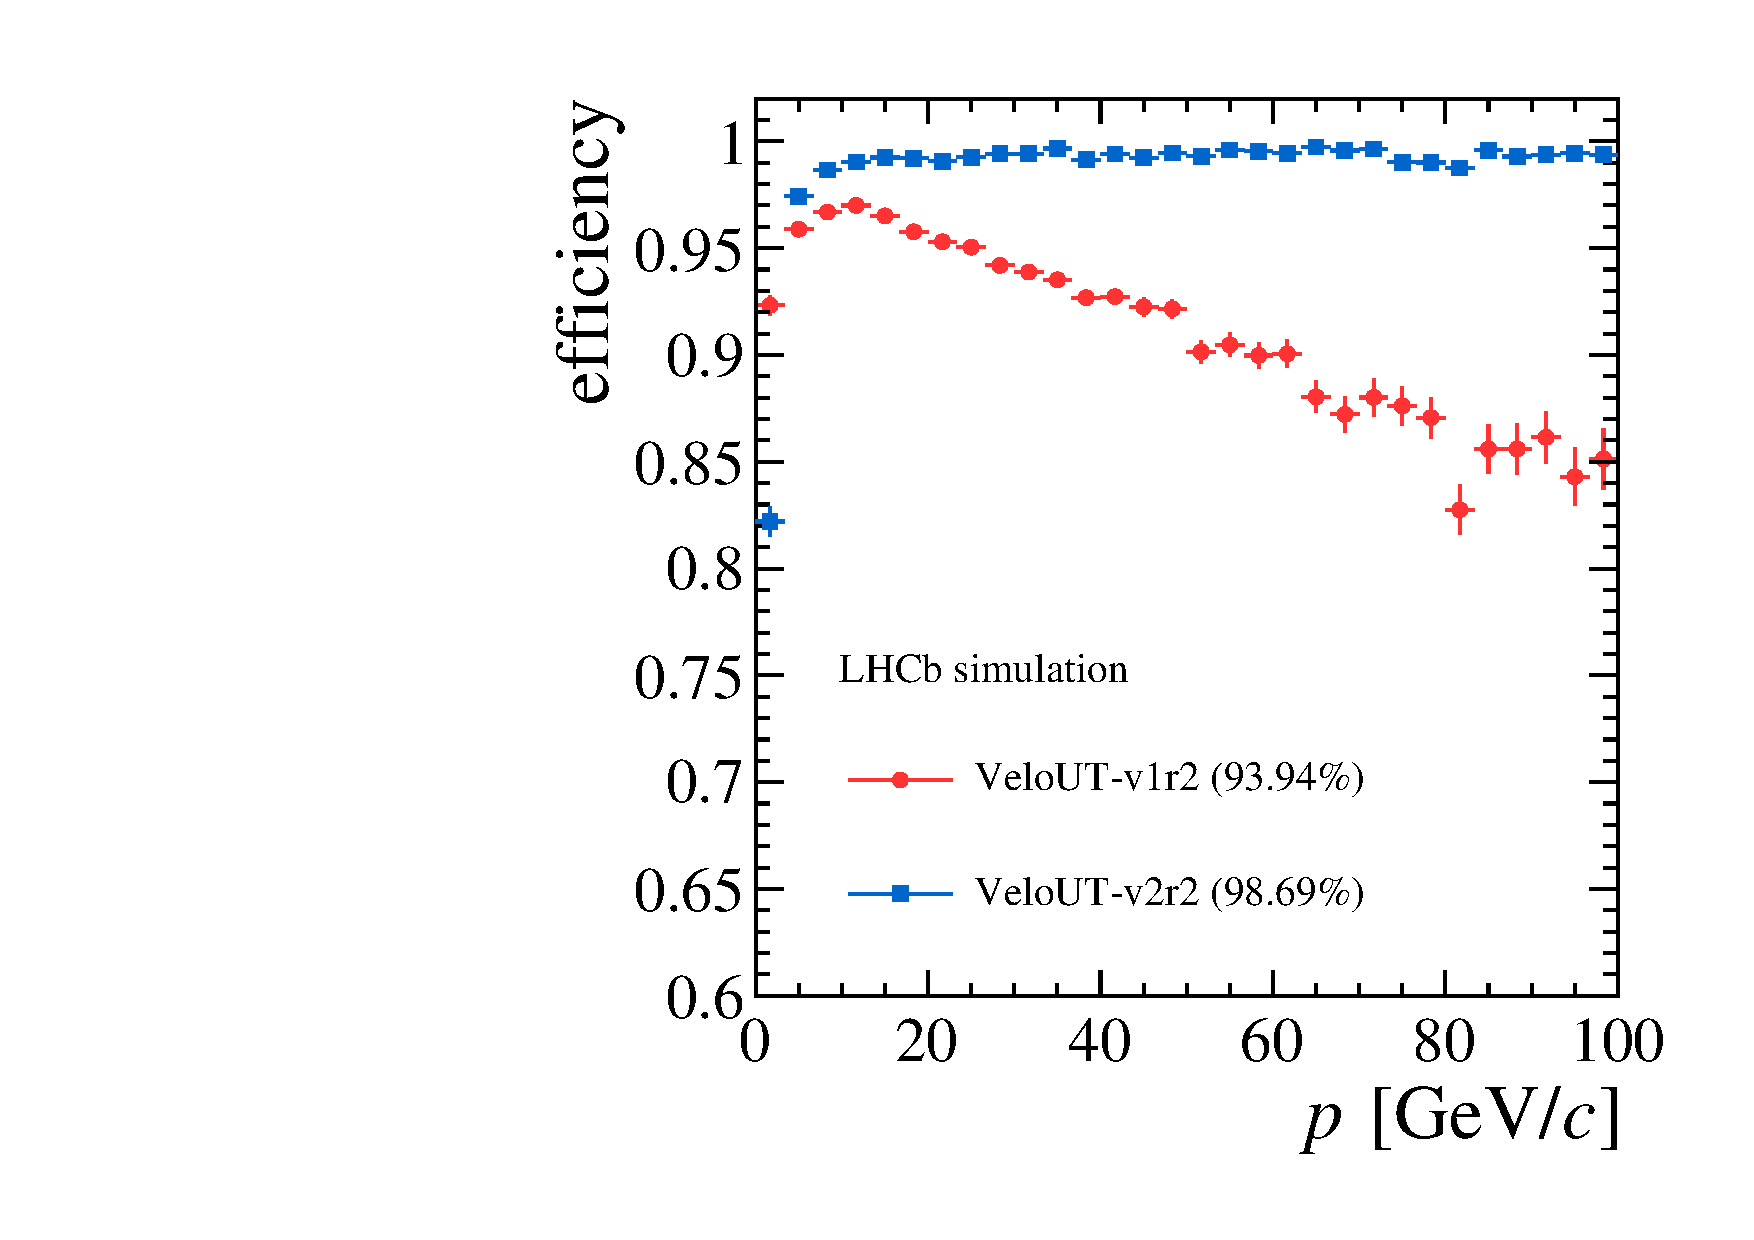
\includegraphics[height=0.475\textheight]{figs/upstream-tracking-upgrade/eff_p_comp.pdf}\\
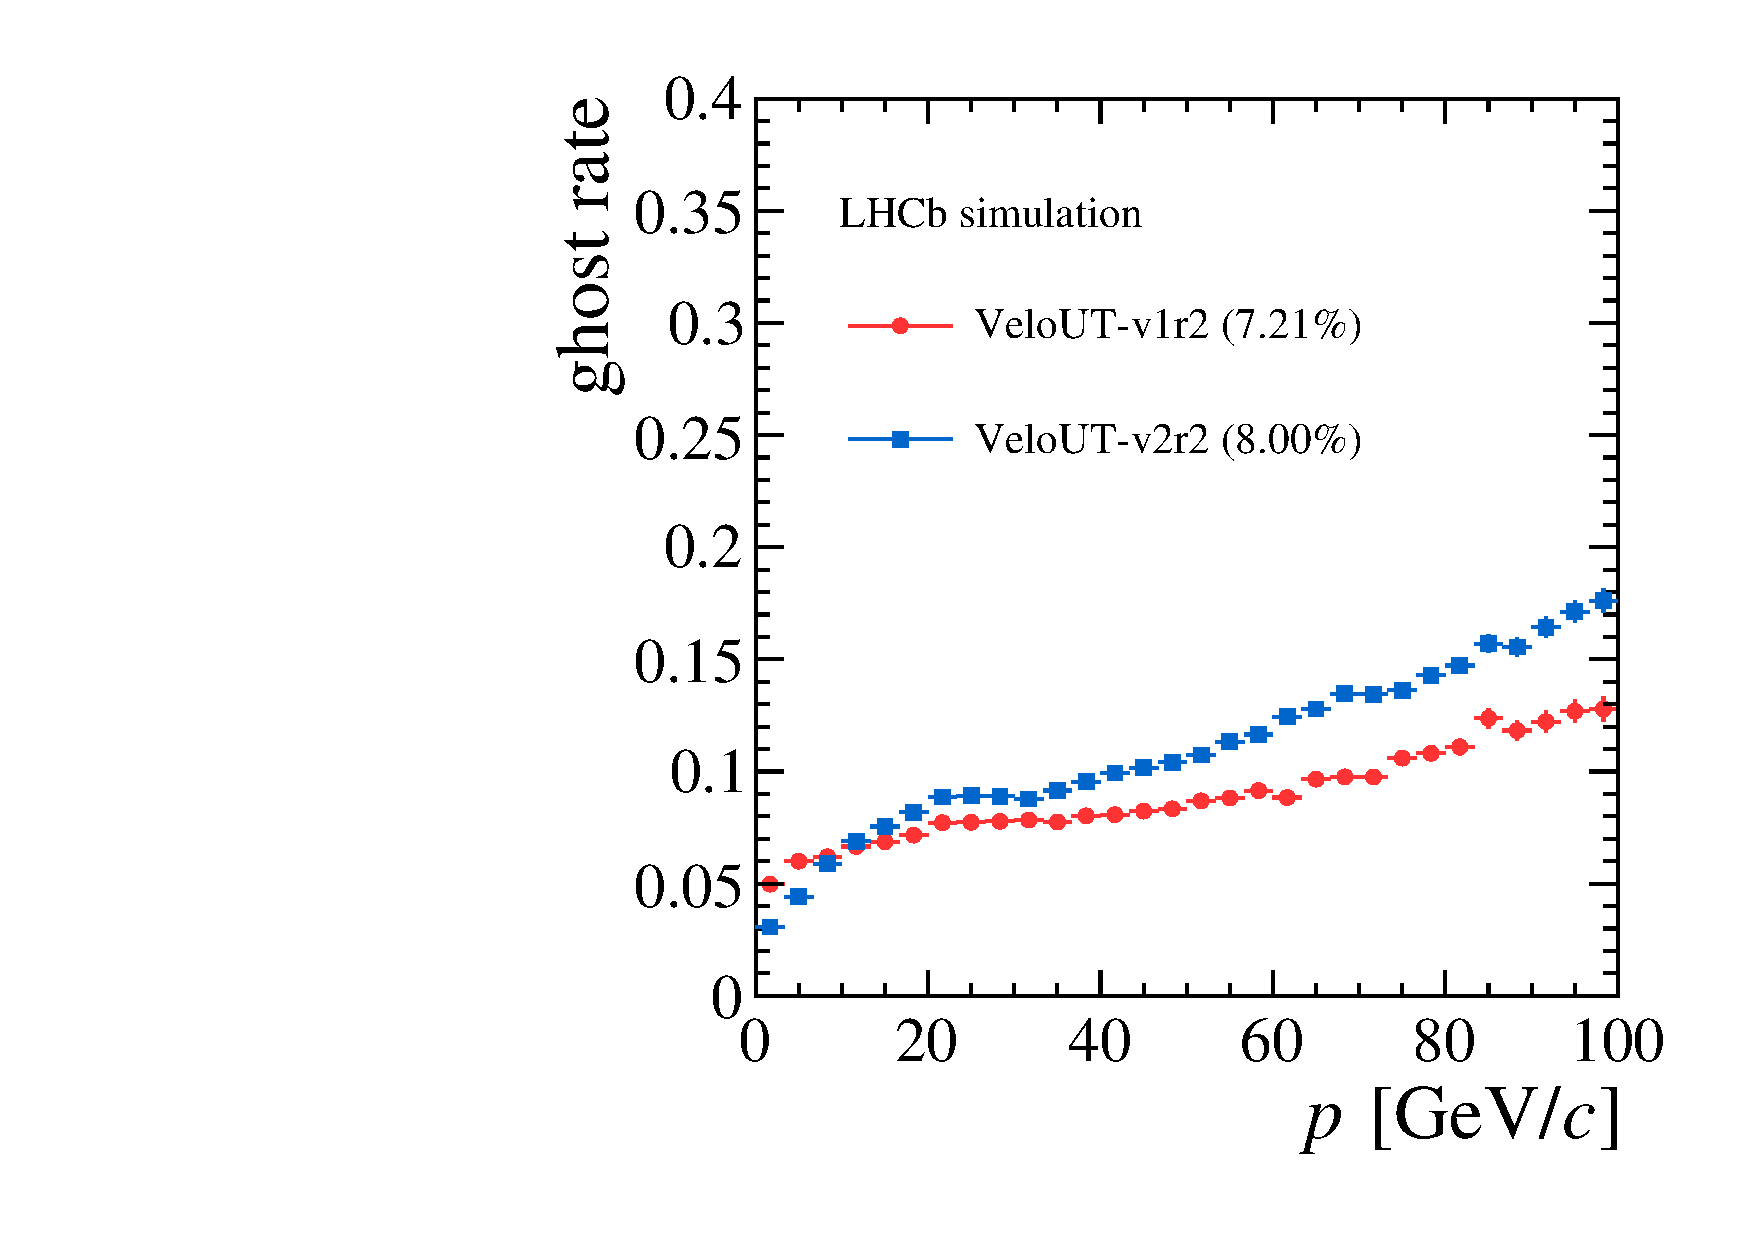
\includegraphics[height=0.475\textheight]{figs/upstream-tracking-upgrade/gr_p_comp.pdf}
\end{figure}
\end{column}
\end{columns}

\end{frame}

%%%%%%%%%%%%%%%%%%%%%%%%%%%%%%%%%%%%%%%%%%%%%%%%%%%%%%%%%%%%%%%%%
%Slide
%%%%%%%%%%%%%%%%%%%%%%%%%%%%%%%%%%%%%%%%%%%%%%%%%%%%%%%%%%%%%%%%%
\begin{frame}{VeloUT-Forward: Optimised peformance}

\begin{columns}
\begin{column}{0.65\textwidth}

\begin{itemize}
  \item[$\blacktriangleright$] Most interested in effect on full tracking sequence (\velo $\to$ [Upstream] $\to$ Forward)
\end{itemize}

\begin{itemize}
  \item[$\blacktriangleright$] Significant reduction in the execution time ($\times$4)
  \item[$\blacktriangleright$] Large reduction in the ghost rate ($\times$3)
  \item[$\blacktriangleright$] Some loss of efficiency ($-0.7$\%)
\end{itemize}

\bigskip

\begin{mdframed}[linecolor=barcolor]
\begin{center}
\resizebox{\columnwidth}{!}{
\begin{tabular}{c|c|c|c}
    & Efficiency [\%] & Ghost rate [\%] & Timing [ms] \\
   \hline
   Velo-Fwd  & 94.10  & 41.55  &  18.28 \\
   VeloUT-Fwd  & 93.37  & 14.08  &  0.81+3.45  \\
 \end{tabular}
 }
\end{center}
\end{mdframed}
\end{column}

\begin{column}{0.35\textwidth}
\centering
\begin{figure}
\vspace*{-1cm}
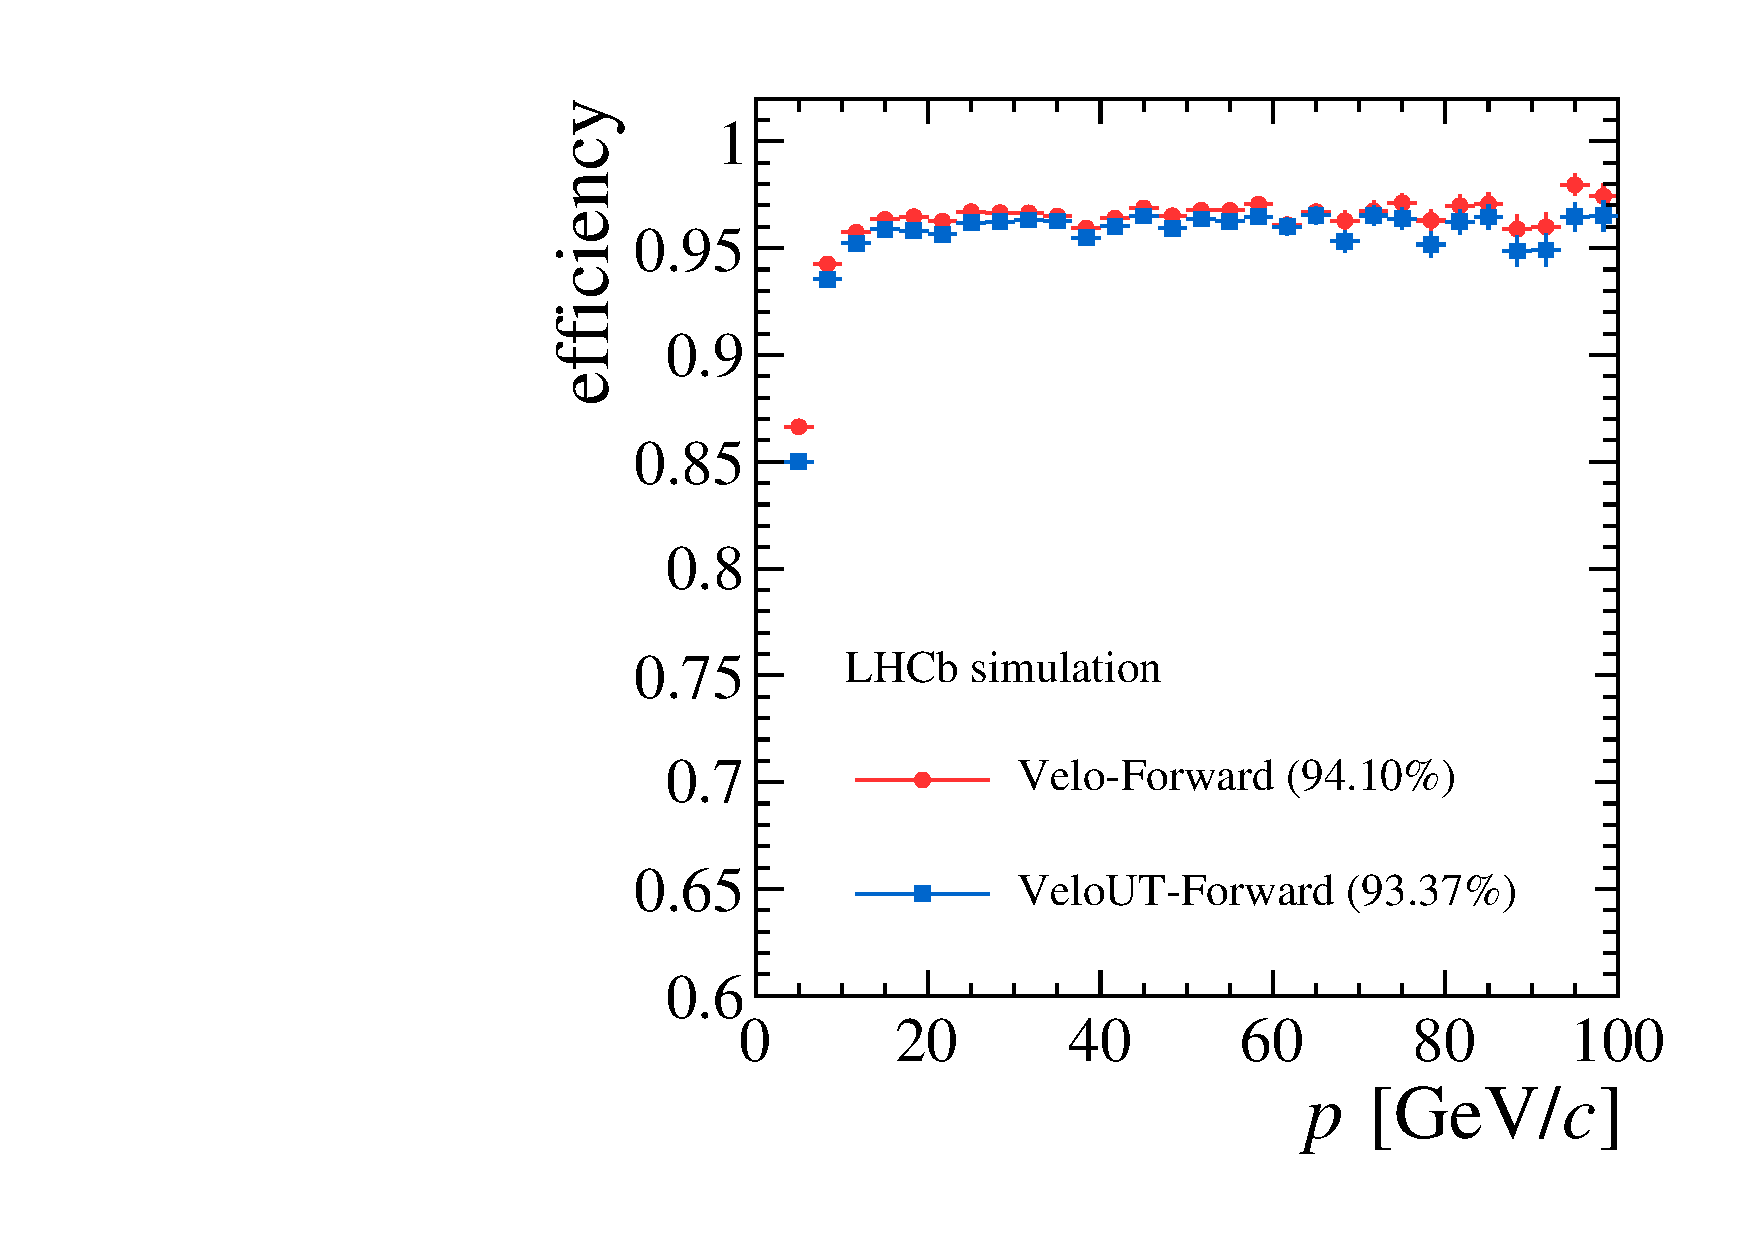
\includegraphics[height=0.475\textheight]{figs/upstream-tracking-upgrade/fwd_eff_p_comp.pdf}\\
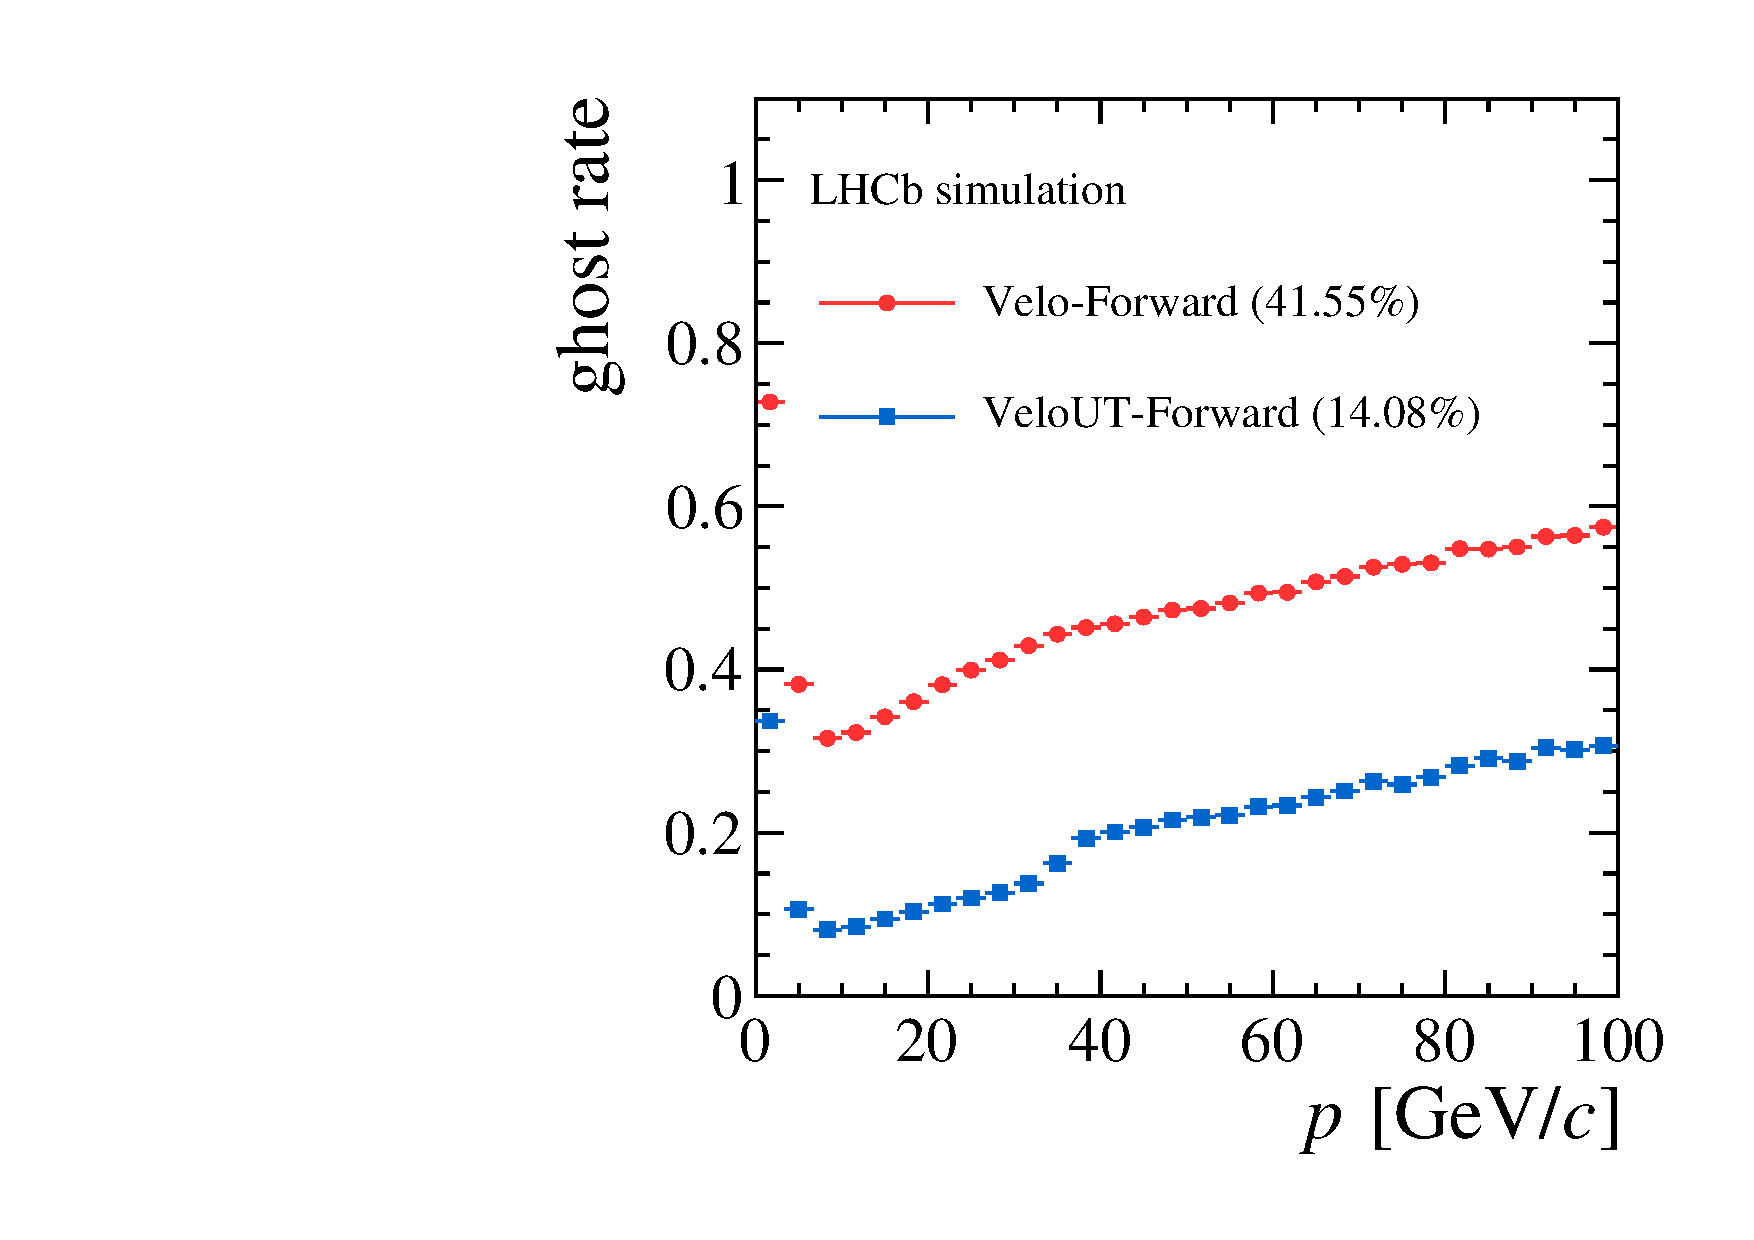
\includegraphics[height=0.475\textheight]{figs/upstream-tracking-upgrade/fwd_gr_p_comp.pdf}
\end{figure}
\end{column}
\end{columns}

\end{frame}

%%%%%%%%%%%%%%%%%%%%%%%%%%%%%%%%%%%%%%%%%%%%%%%%%%%%%%%%%%%%%%%%%
%Slide
%%%%%%%%%%%%%%%%%%%%%%%%%%%%%%%%%%%%%%%%%%%%%%%%%%%%%%%%%%%%%%%%%
\begin{frame}{Upstream tracking for the Upgrade: Summary}

\begin{columns}
\begin{column}{0.75\textwidth}
\begin{itemize}
  \item[$\blacktriangleright$] Vast improvements in the performance of the \velout algorithm
  \item[$\blacktriangleright$] Leads to subsequent improvement to the overall tracking sequence
  \item[\ding{72}] Adopted into the default tracking sequence for the \lhcb Upgrade
\end{itemize}
\end{column}
\begin{column}{0.25\textwidth}
%\centering
\href{https://cds.cern.ch/record/1624070}{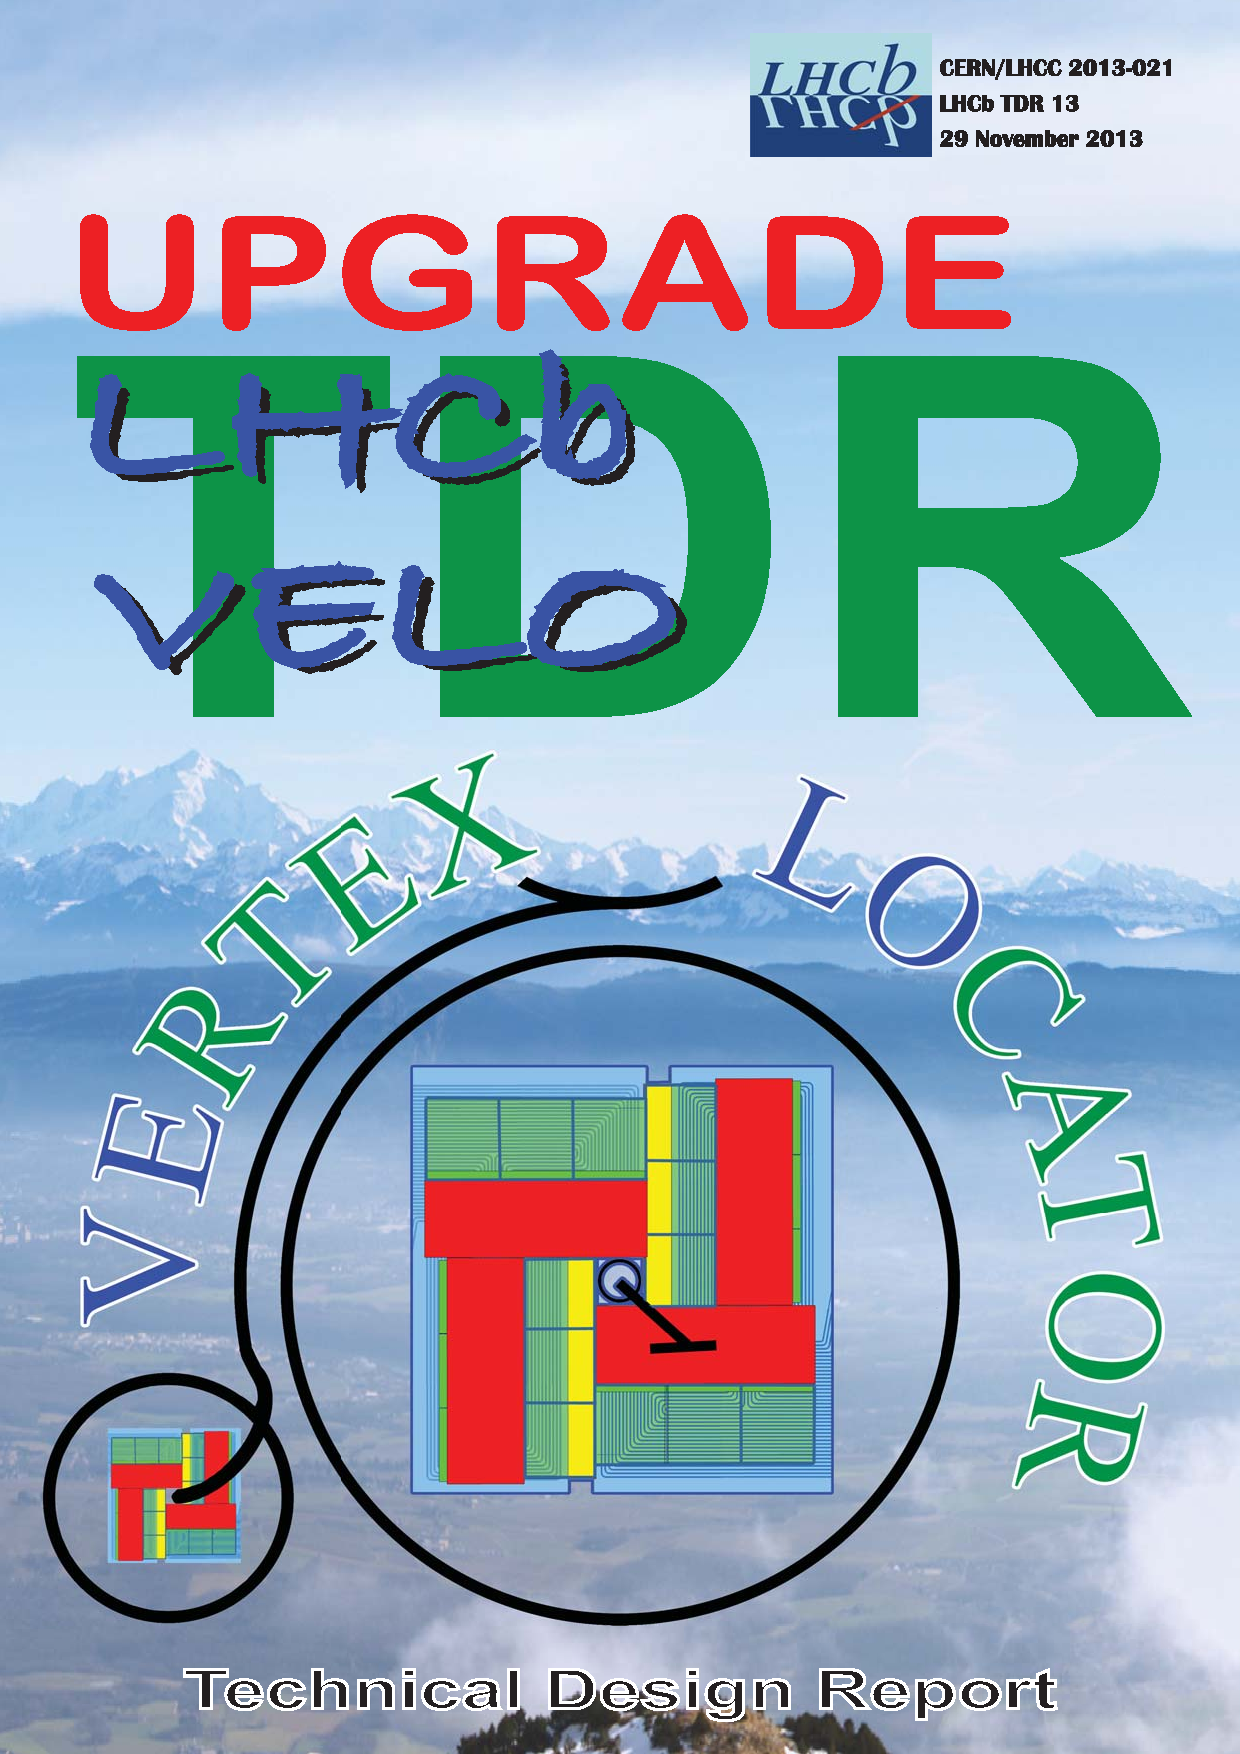
\includegraphics[width=0.48\textwidth]{figs/VELO.pdf}}
\href{https://cds.cern.ch/record/1624074}{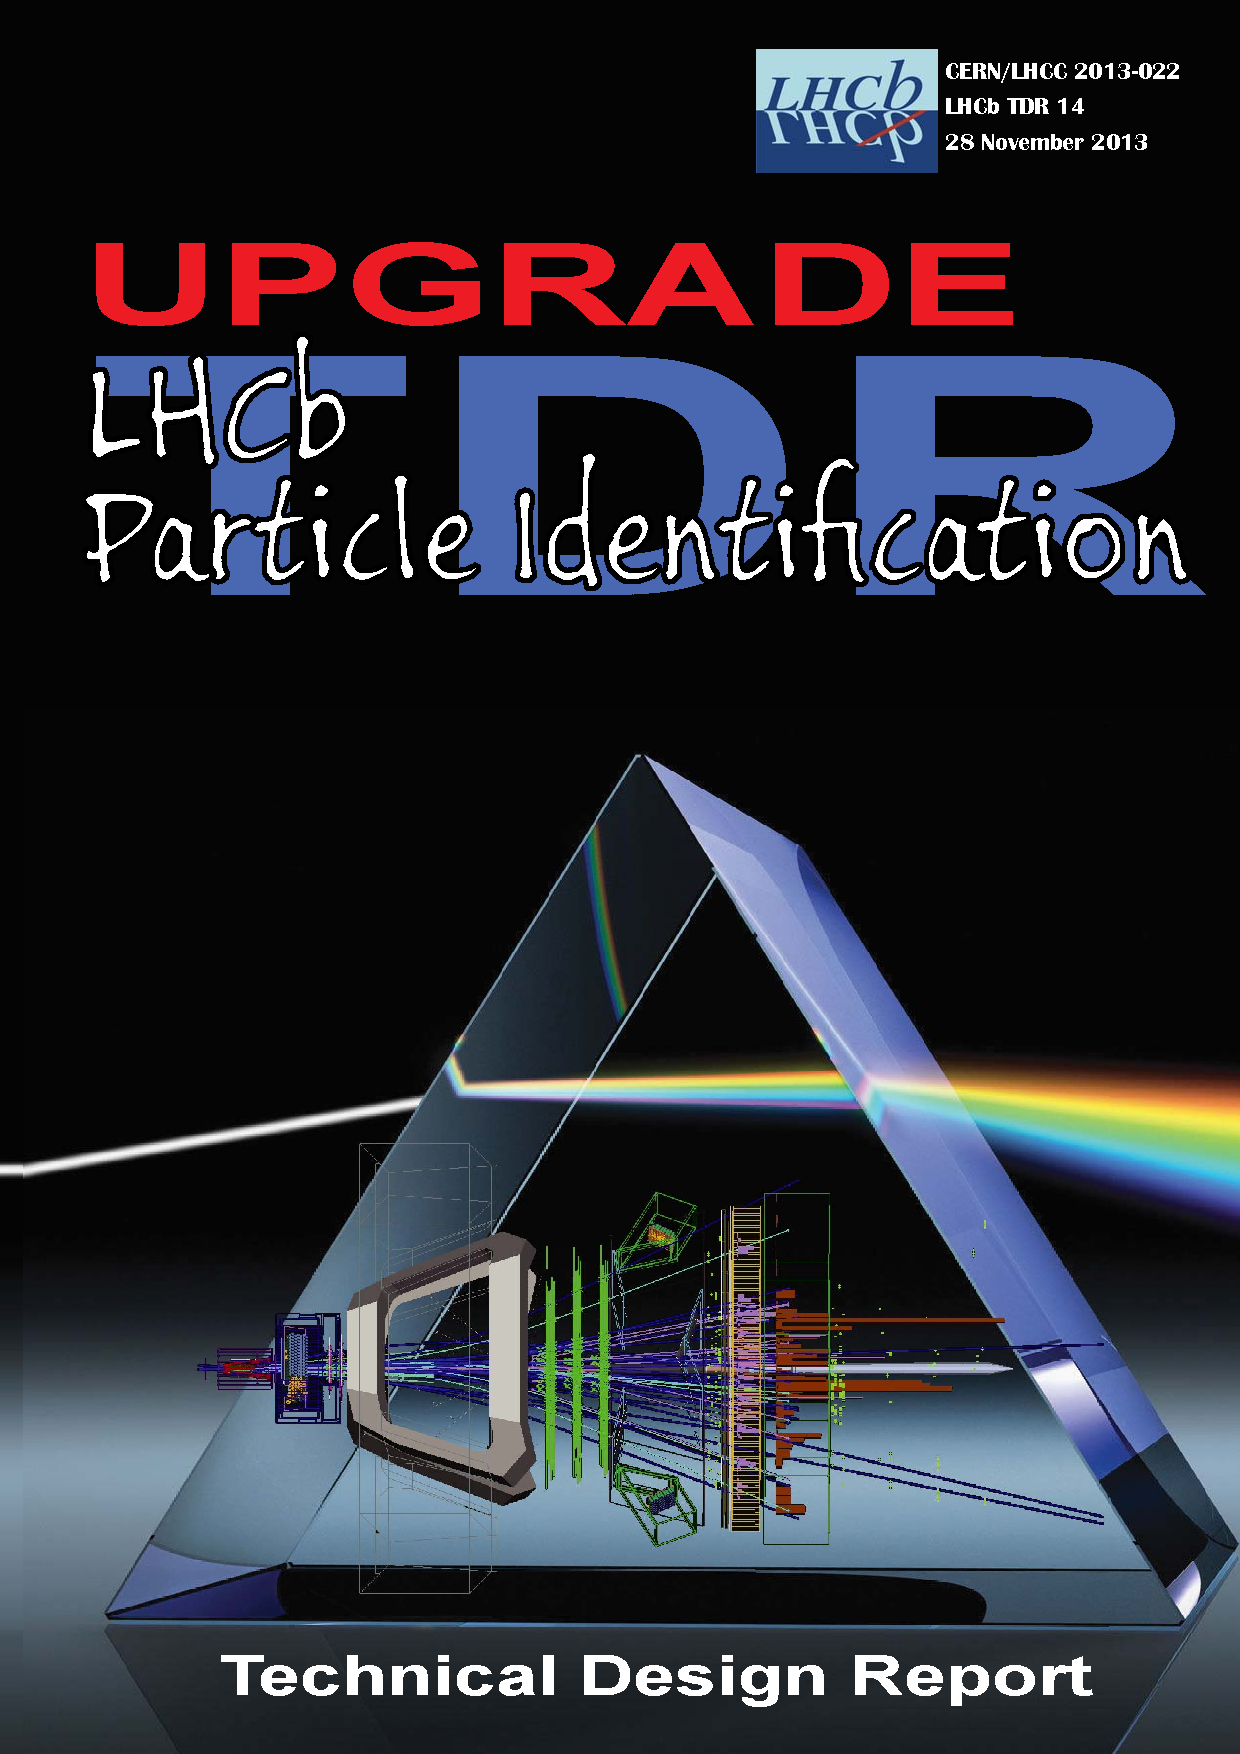
\includegraphics[width=0.48\textwidth]{figs/PID.pdf}}\\
\href{https://cds.cern.ch/record/1647400}{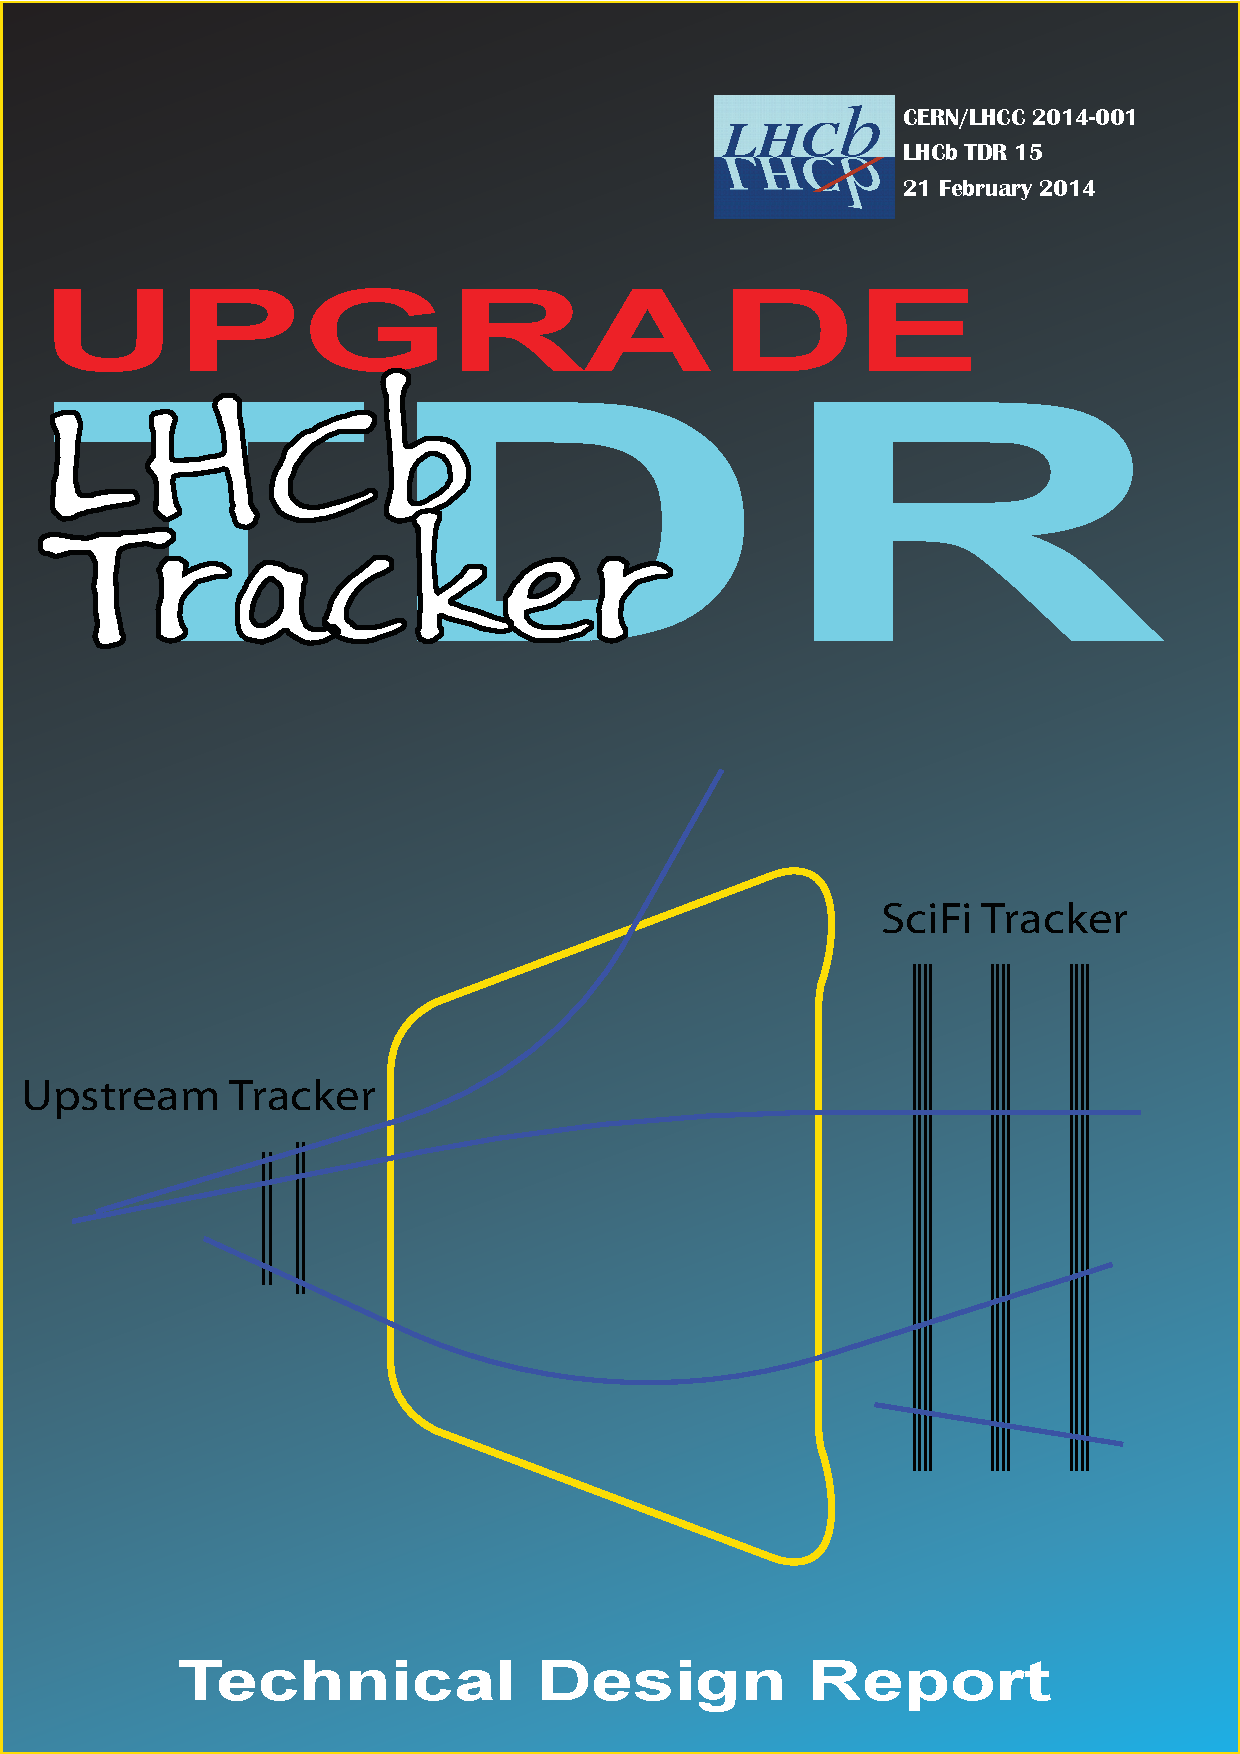
\includegraphics[width=0.48\textwidth]{figs/Tracking.pdf}}
\href{https://cds.cern.ch/record/1701361}{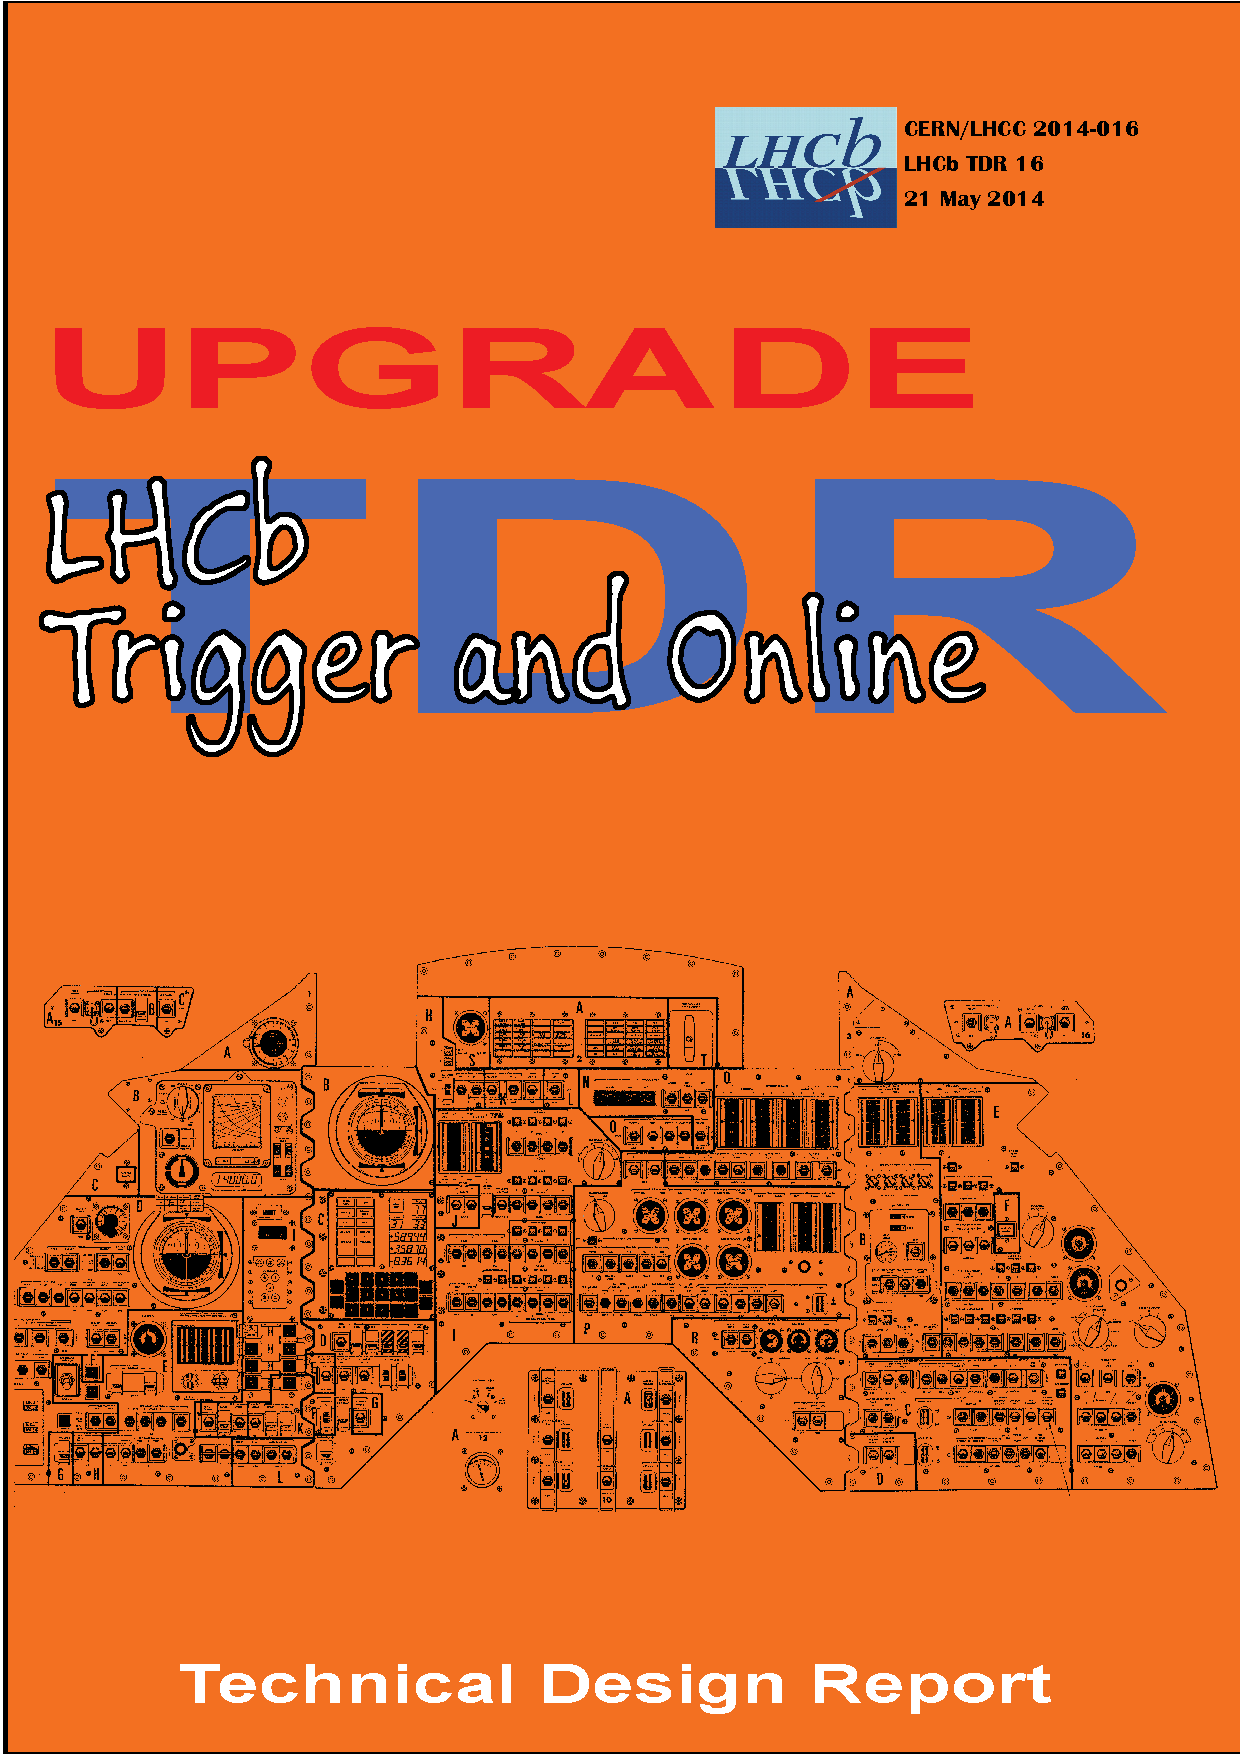
\includegraphics[width=0.48\textwidth]{figs/Trigger.pdf}}
\end{column}
\end{columns}

\bigskip\bigskip

\begin{itemize}
\item[\ding{72}] \lhcb will become the first hadron collider experiment to operate a software-only trigger
\end{itemize}

\end{frame}

%%%%%%%%%%%%%%%%%%%%%%%%%%%%%%%%%%%%%%%%%%%%%%%%%%%%%%%%%%%%%%%%%
%Slide
%%%%%%%%%%%%%%%%%%%%%%%%%%%%%%%%%%%%%%%%%%%%%%%%%%%%%%%%%%%%%%%%%
{\usebackgroundtemplate{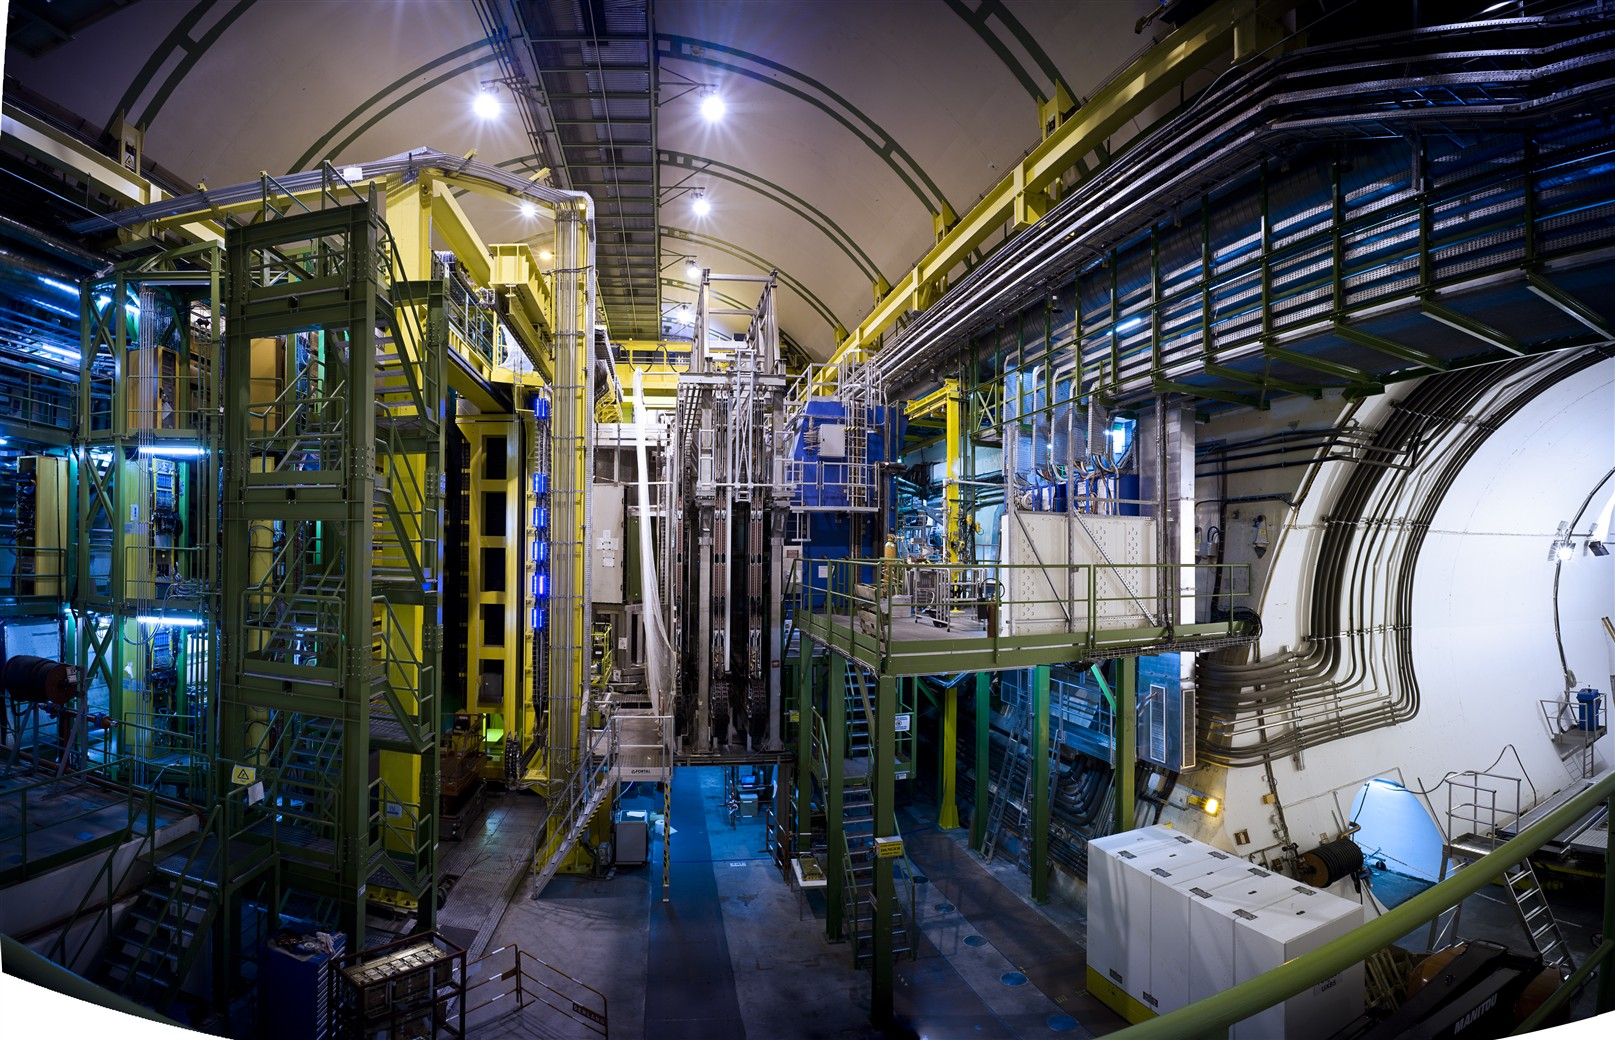
\includegraphics[width=1.05\paperwidth]{figs/cavern.jpg}}
 
 \begin{frame}[plain]
 \vspace{8.75cm}
 \hspace{-0.75cm}
 \huge\color{anti-flashwhite}{The decay \BdToKpimm}
 \end{frame}
}

%%%%%%%%%%%%%%%%%%%%%%%%%%%%%%%%%%%%%%%%%%%%%%%%%%%%%%%%%%%%%%%%%
%Slide
%%%%%%%%%%%%%%%%%%%%%%%%%%%%%%%%%%%%%%%%%%%%%%%%%%%%%%%%%%%%%%%%%
\begin{frame}{Reminder: Rare decays as a probe for NP}
  \begin{columns}
    \begin{column}{0.6\textwidth}
      \begin{itemize}
      \item[$\blacktriangleright$] The decay \BdToKpimm is an example of a \btosmm processes that proceeds via loop diagrams in SM
      \item[$\blacktriangleright$] New, heavy particles in SM extensions can enter the loop and modify observables 
      \begin{itemize}
        \item[\ding{70}] e.g. enhance/suppress branching fractions or alter angular distributions%, new sources of \CP violation
      \end{itemize}
      \item[$\blacktriangleright$] Can compare measurements to SM predictions
      \end{itemize}
    \end{column}
    
    \begin{column}{0.4\textwidth}
      \vspace{-1cm}
      \begin{myenv}{\color{bleudefrance}{SM}}[linecolor=bleudefrance]
      \centering
      \begin{tikzpicture}
      \node[anchor=south west,inner sep=0](image) at (0,0) {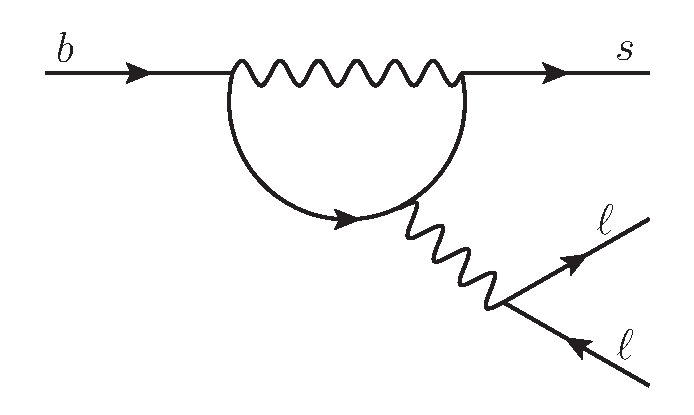
\includegraphics[width=0.7\textwidth]{figs/theory/btosll_penguin.eps}};
      \begin{scope}[x={(image.south east)},y={(image.north west)}]
      %\draw[help lines,xstep=.1,ystep=.1] (0,0) grid (1,1);
      \node[draw=none,bleudefrance] at (0.53,0.98) {\scriptsize \Wm};
      \node[draw=none,bleudefrance] at (0.3,0.6) {\scriptsize \tquark};
      \node[draw=none,bleudefrance] at (0.56,0.27) {\scriptsize {\small\Pgamma},$\Z^{0}$};
      \end{scope}
      \end{tikzpicture}
      \begin{tikzpicture}
      \node[anchor=south west,inner sep=0](image) at (0,0) {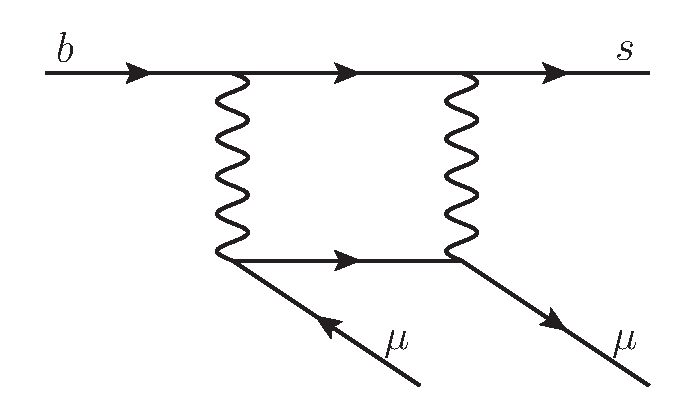
\includegraphics[width=0.7\textwidth]{figs/theory/btosll_box.eps}};
      \begin{scope}[x={(image.south east)},y={(image.north west)}]
      %\draw[help lines,xstep=.1,ystep=.1] (0,0) grid (1,1);
      \node[draw=none,bleudefrance] at (0.5,0.95) {\scriptsize \tquark};
      \node[draw=none,bleudefrance] at (0.23,0.6) {\scriptsize \Wm};
      \node[draw=none,bleudefrance] at (0.8,0.6) {\scriptsize \Wp};
      \node[draw=none,bleudefrance] at (0.5,0.45) {\scriptsize \Pnu};
      \end{scope}
      \end{tikzpicture}
      \end{myenv}
    \end{column}
    \end{columns}

    \begin{myenv}{\color{bostonuniversityred}{NP}}[linecolor=bostonuniversityred]
      \centering
      \begin{tikzpicture}
      \node[anchor=south west,inner sep=0](image) at (0,0) {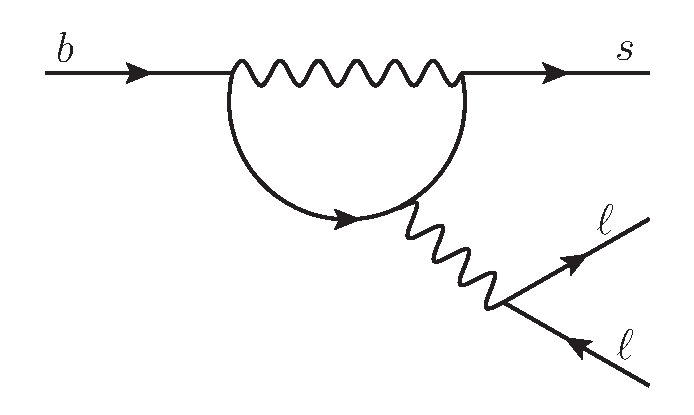
\includegraphics[width=0.3\textwidth]{figs/theory/btosll_penguin.eps}};
      \begin{scope}[x={(image.south east)},y={(image.north west)}]
      %\draw[help lines,xstep=.1,ystep=.1] (0,0) grid (1,1);
      \node[draw=none,bostonuniversityred] at (0.5,0.96) {\small ?};
      \node[draw=none,bostonuniversityred] at (0.3,0.6) {\small ?};
      \node[draw=none,bostonuniversityred] at (0.58,0.27) {\small ?};
      \end{scope}
      \end{tikzpicture}
      \begin{tikzpicture}
      \node[anchor=south west,inner sep=0](image) at (0,0) {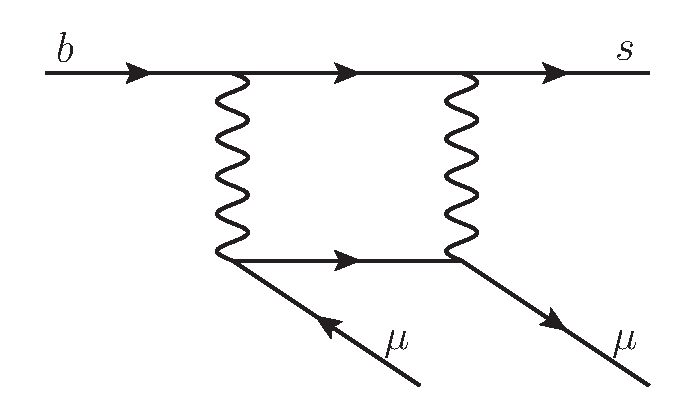
\includegraphics[width=0.3\textwidth]{figs/theory/btosll_box.eps}};
      \begin{scope}[x={(image.south east)},y={(image.north west)}]
      %\draw[help lines,xstep=.1,ystep=.1] (0,0) grid (1,1);
      \node[draw=none,bostonuniversityred] at (0.5,0.97) {\small ?};
      \node[draw=none,bostonuniversityred] at (0.25,0.6) {\small ?};
      \node[draw=none,bostonuniversityred] at (0.8,0.6) {\small ?};
      \node[draw=none,bostonuniversityred] at (0.5,0.49) {\small ?};
      \end{scope}
      \end{tikzpicture}
    \begin{tikzpicture}
      \node[anchor=south west,inner sep=0](image) at (0,0) {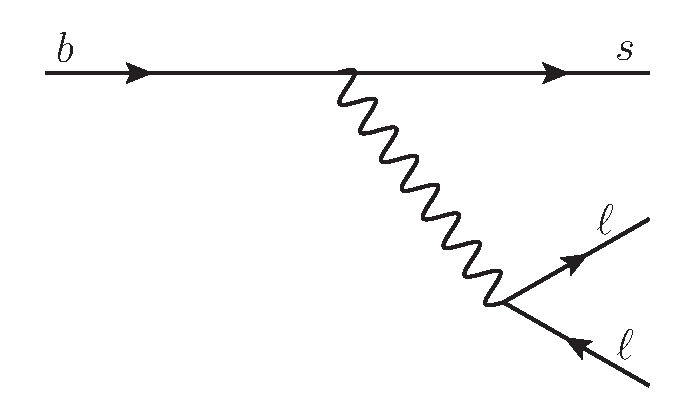
\includegraphics[width=0.3\textwidth]{figs/theory/btosll_zprime.eps}};
      \begin{scope}[x={(image.south east)},y={(image.north west)}]
      %\draw[help lines,xstep=.1,ystep=.1] (0,0) grid (1,1);
      \node[draw=none,bostonuniversityred] at (0.55,0.45) {\small ?};
      \end{scope}
      \end{tikzpicture}
    \end{myenv}

\end{frame}

%%%%%%%%%%%%%%%%%%%%%%%%%%%%%%%%%%%%%%%%%%%%%%%%%%%%%%%%%%%%%%%%%
%Slide
%%%%%%%%%%%%%%%%%%%%%%%%%%%%%%%%%%%%%%%%%%%%%%%%%%%%%%%%%%%%%%%%%
\begin{frame}{Previous measurements: Differential branching fractions ($\deriv\BF/\deriv\qsq$)}

\begin{itemize}
  \item[$\blacktriangleright$] Differential branching fractions of different \btosmm processes
  \begin{itemize}
    \item[\ding{70}] Measured as a function of $\qsq\equiv m_{\mu\mu}^{2}$
  \end{itemize}
  %\item[$\blacktriangleright$] Large LHCb datasets allow for precise measurements of the differential branching fractions of \btosmm processes
  \item[\ding{72}] Results point towards lower rates than predicted by the SM
\end{itemize}

\begin{center}
\begin{tikzpicture}
 \centering
 \node[anchor=south west,inner sep=0](image) at (0,0) {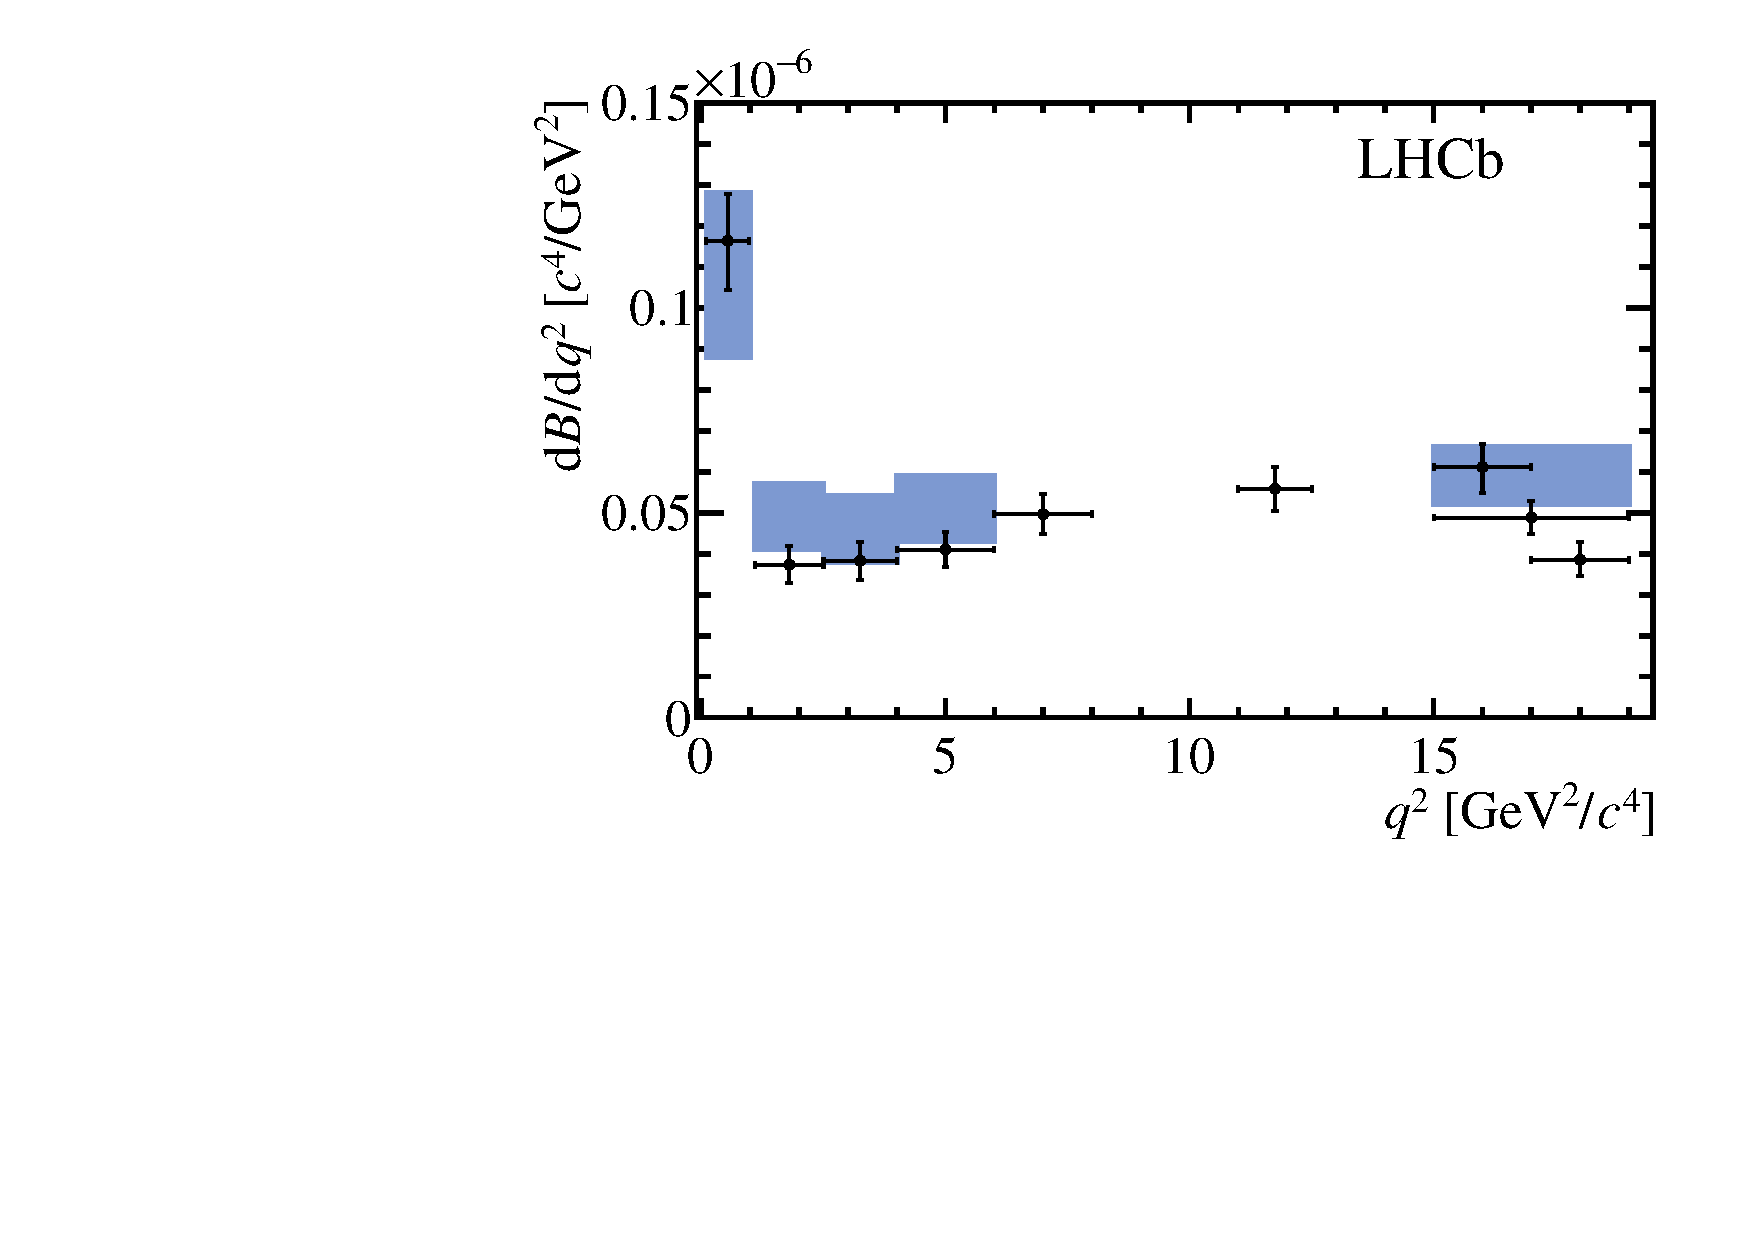
\includegraphics[height=0.33\textheight]{figs/BFs/BdKstmm.pdf}};
 \begin{scope}[x={(image.south east)},y={(image.north west)}]
  %\draw[help lines,xstep=.1,ystep=.1] (0,0) grid (1,1);
  \node[draw=none] at (0.55,0.98) {\tiny \BdToKstmm};
 \end{scope}
\end{tikzpicture}
\begin{tikzpicture}
 \centering
 \node[anchor=south west,inner sep=0](image) at (0,0) {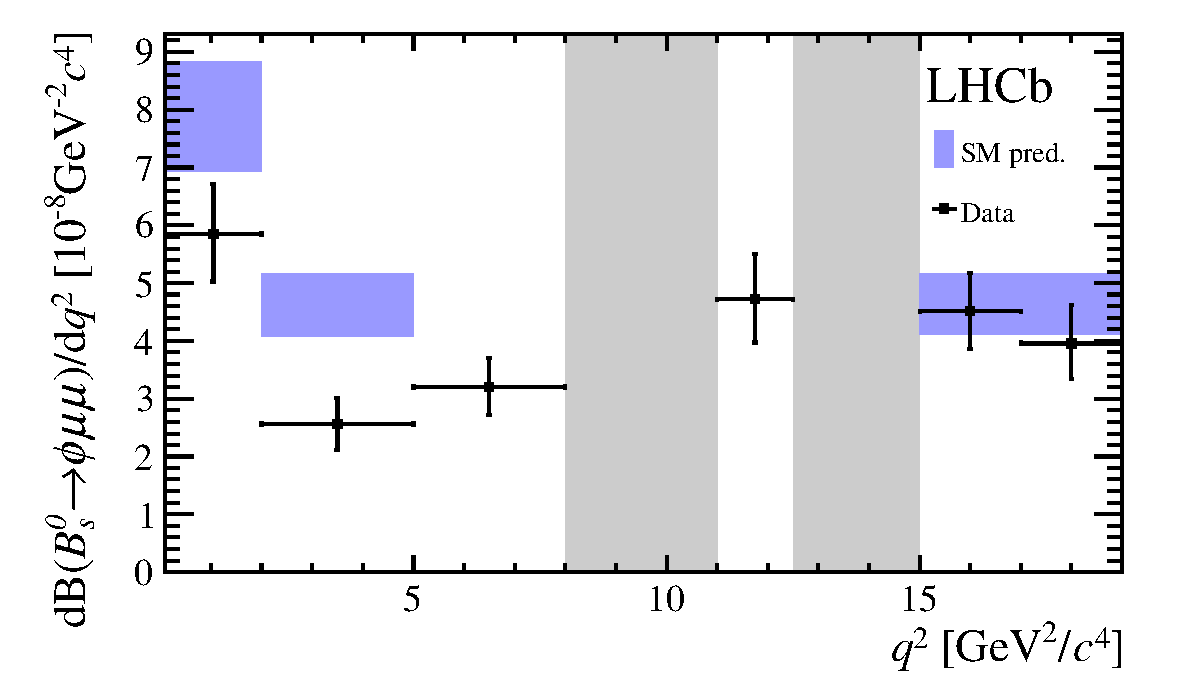
\includegraphics[height=0.33\textheight]{figs/BFs/BsPhiMM.pdf}};
 \begin{scope}[x={(image.south east)},y={(image.north west)}]
  %\draw[help lines,xstep=.1,ystep=.1] (0,0) grid (1,1);
  \node[draw=none] at (0.55,1.01) {\tiny \BsTophimm};
 \end{scope}
\end{tikzpicture}
\begin{tikzpicture}
 \centering
 \node[anchor=south west,inner sep=0](image) at (0,0) {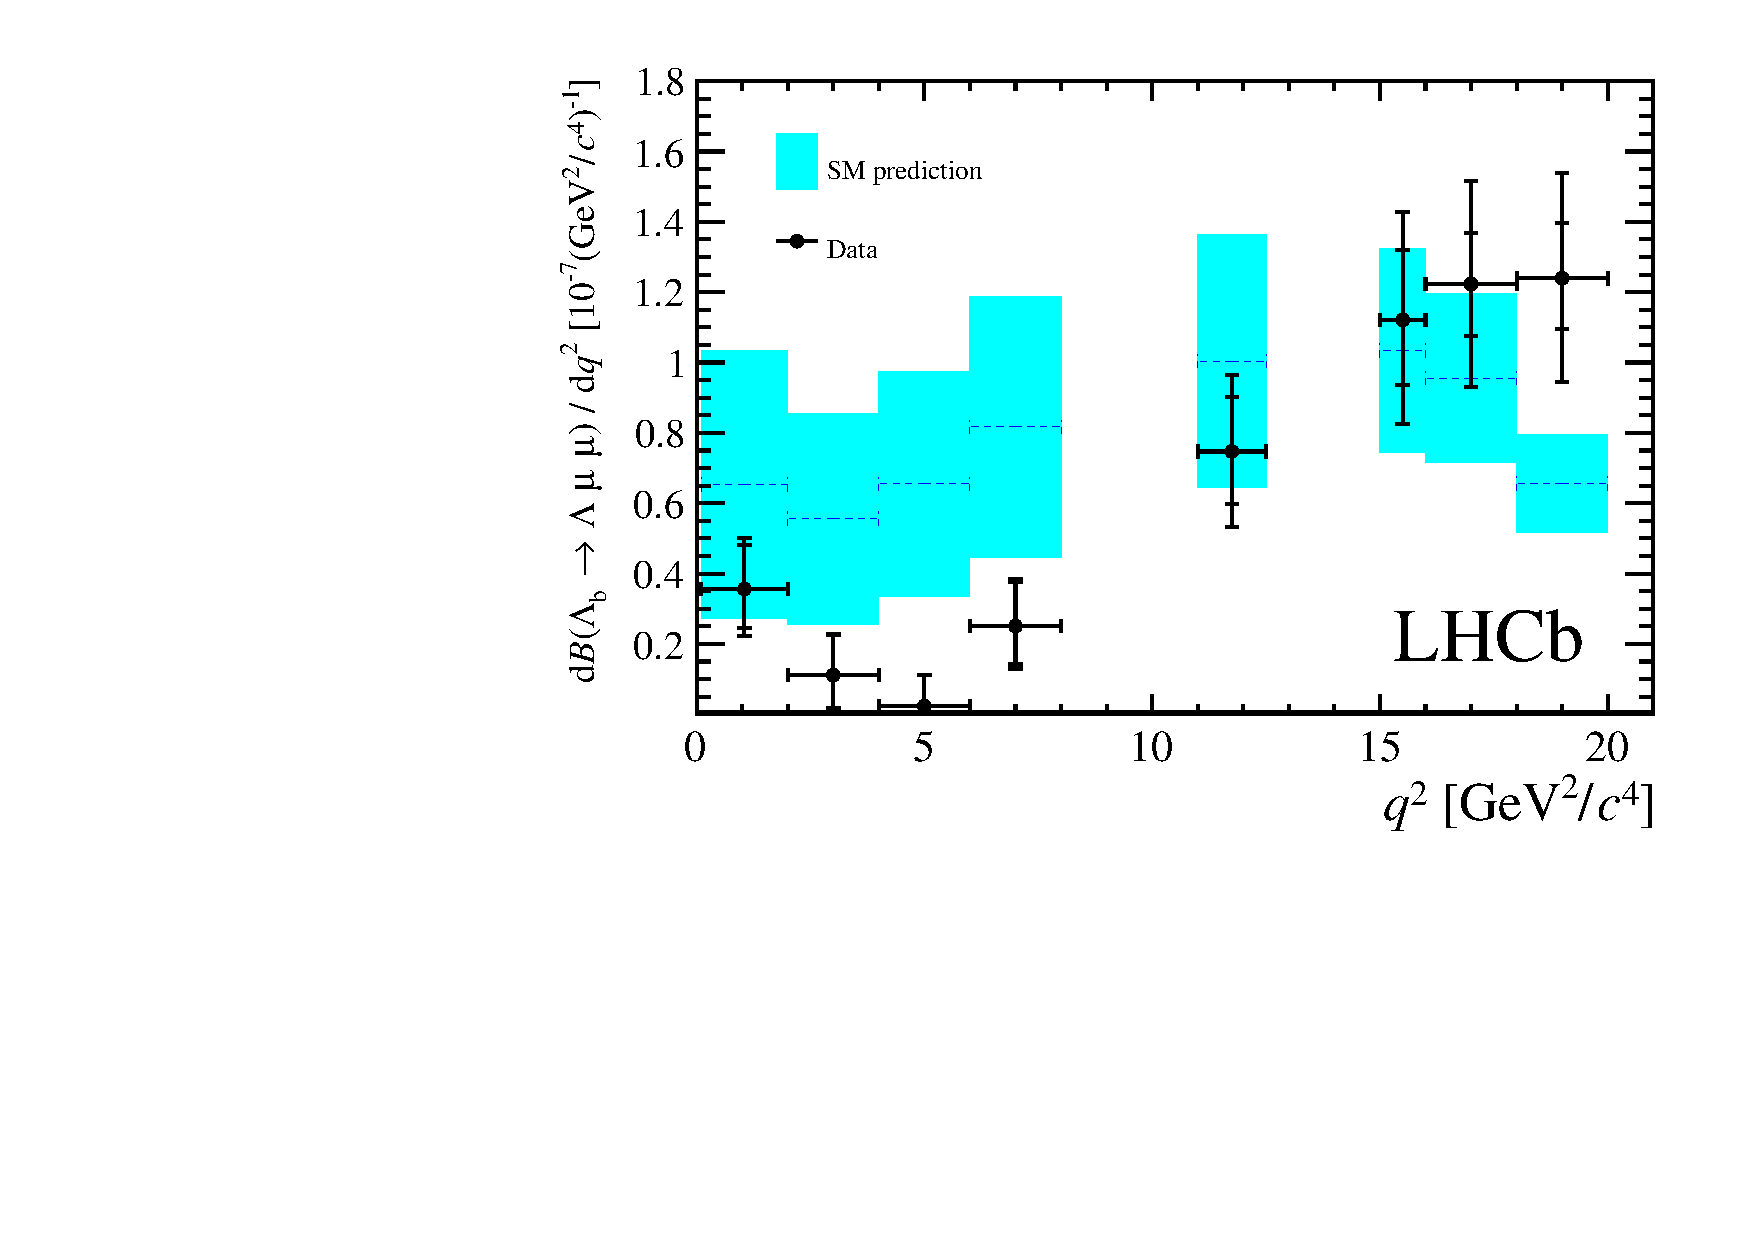
\includegraphics[height=0.33\textheight]{figs/BFs/LbLMM.pdf}};
 \begin{scope}[x={(image.south east)},y={(image.north west)}]
  %\draw[help lines,xstep=.1,ystep=.1] (0,0) grid (1,1);
  \node[draw=none] at (0.55,1.01) {\tiny \decay{\Lb}{\Lz\mumu}};
 \end{scope}
\end{tikzpicture}
\begin{tikzpicture}
 \centering
 \node[anchor=south west,inner sep=0](image) at (0,0) {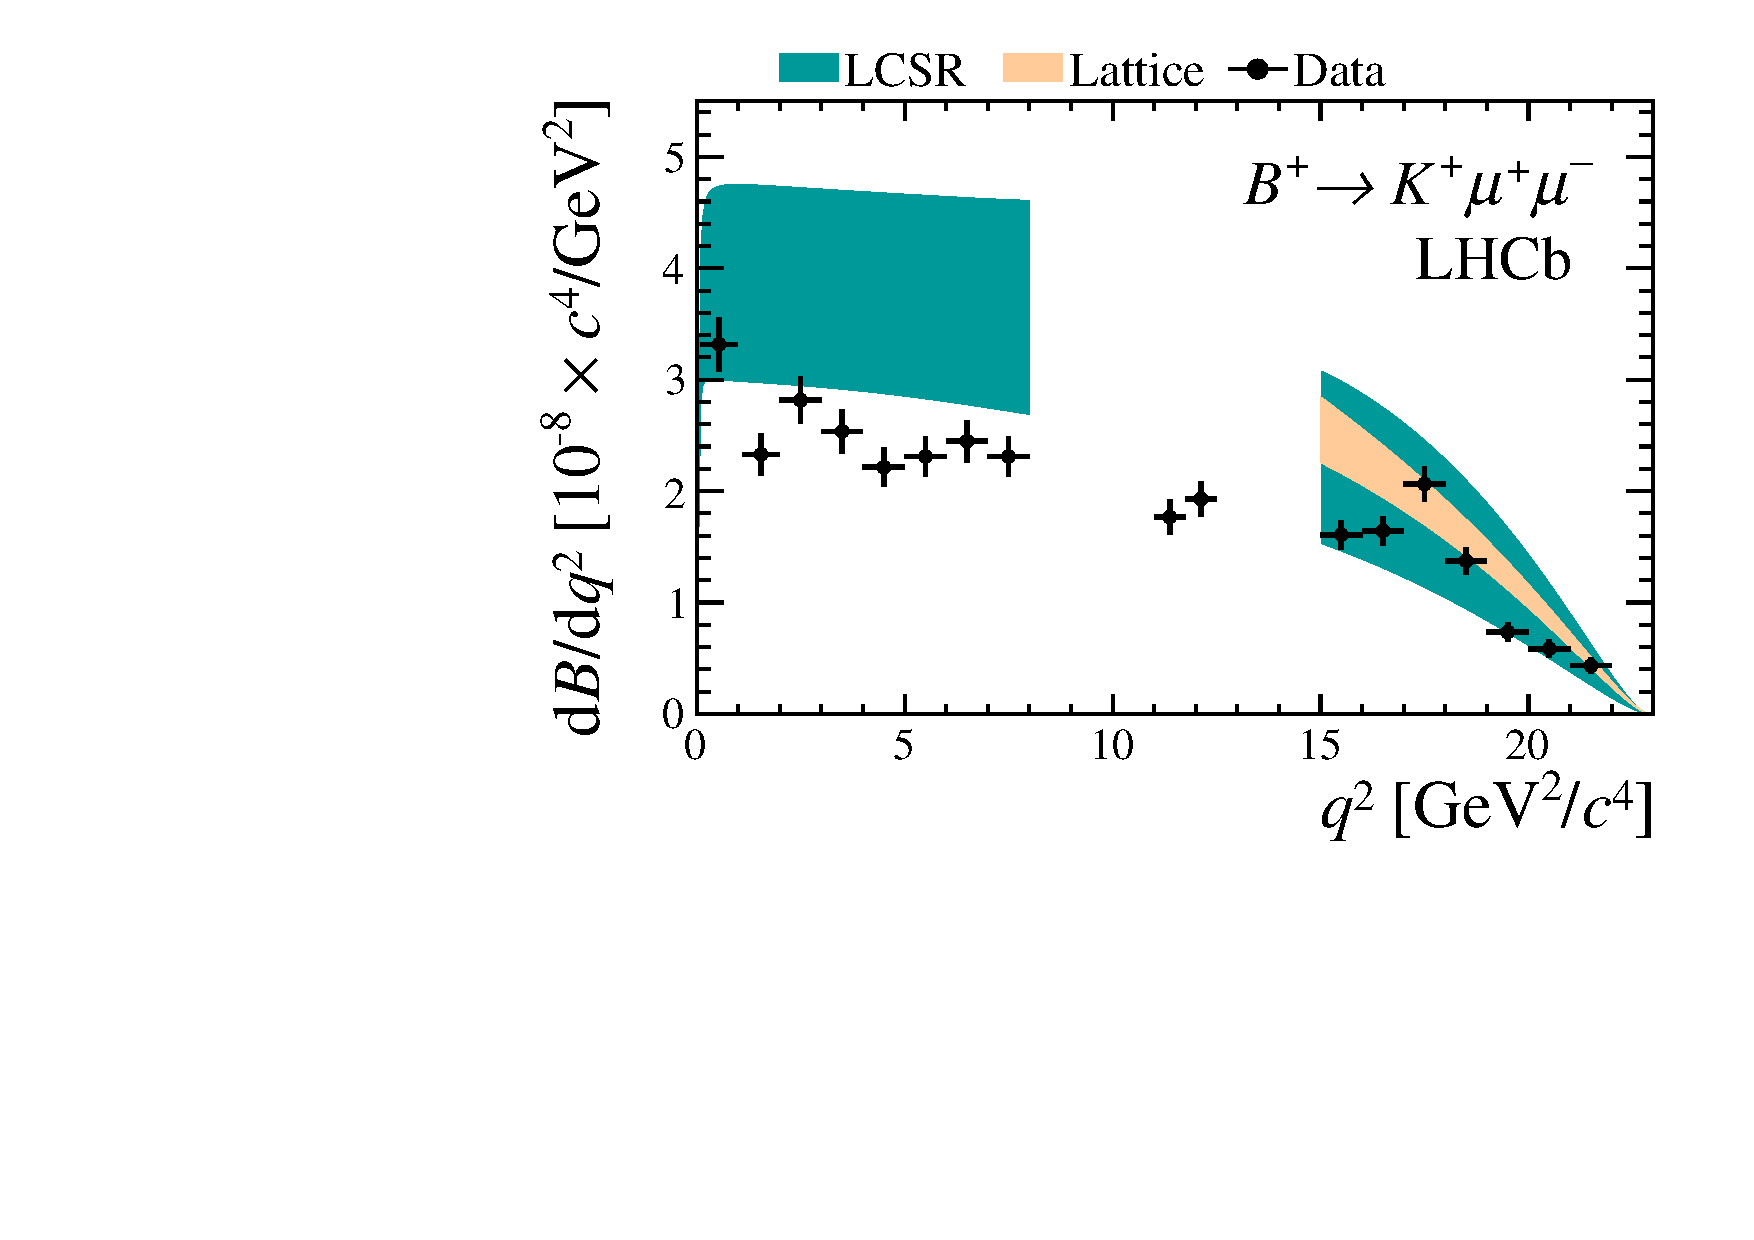
\includegraphics[height=0.33\textheight]{figs/BFs/kmumu_BF.pdf}};
 \begin{scope}[x={(image.south east)},y={(image.north west)}]
  %\draw[help lines,xstep=.1,ystep=.1] (0,0) grid (1,1);
  %\node[draw=none] at (0.45,0.85) {\tiny \BsTophimm};
 \end{scope}
\end{tikzpicture}
\begin{tikzpicture}
 \centering
 \node[anchor=south west,inner sep=0](image) at (0,0) {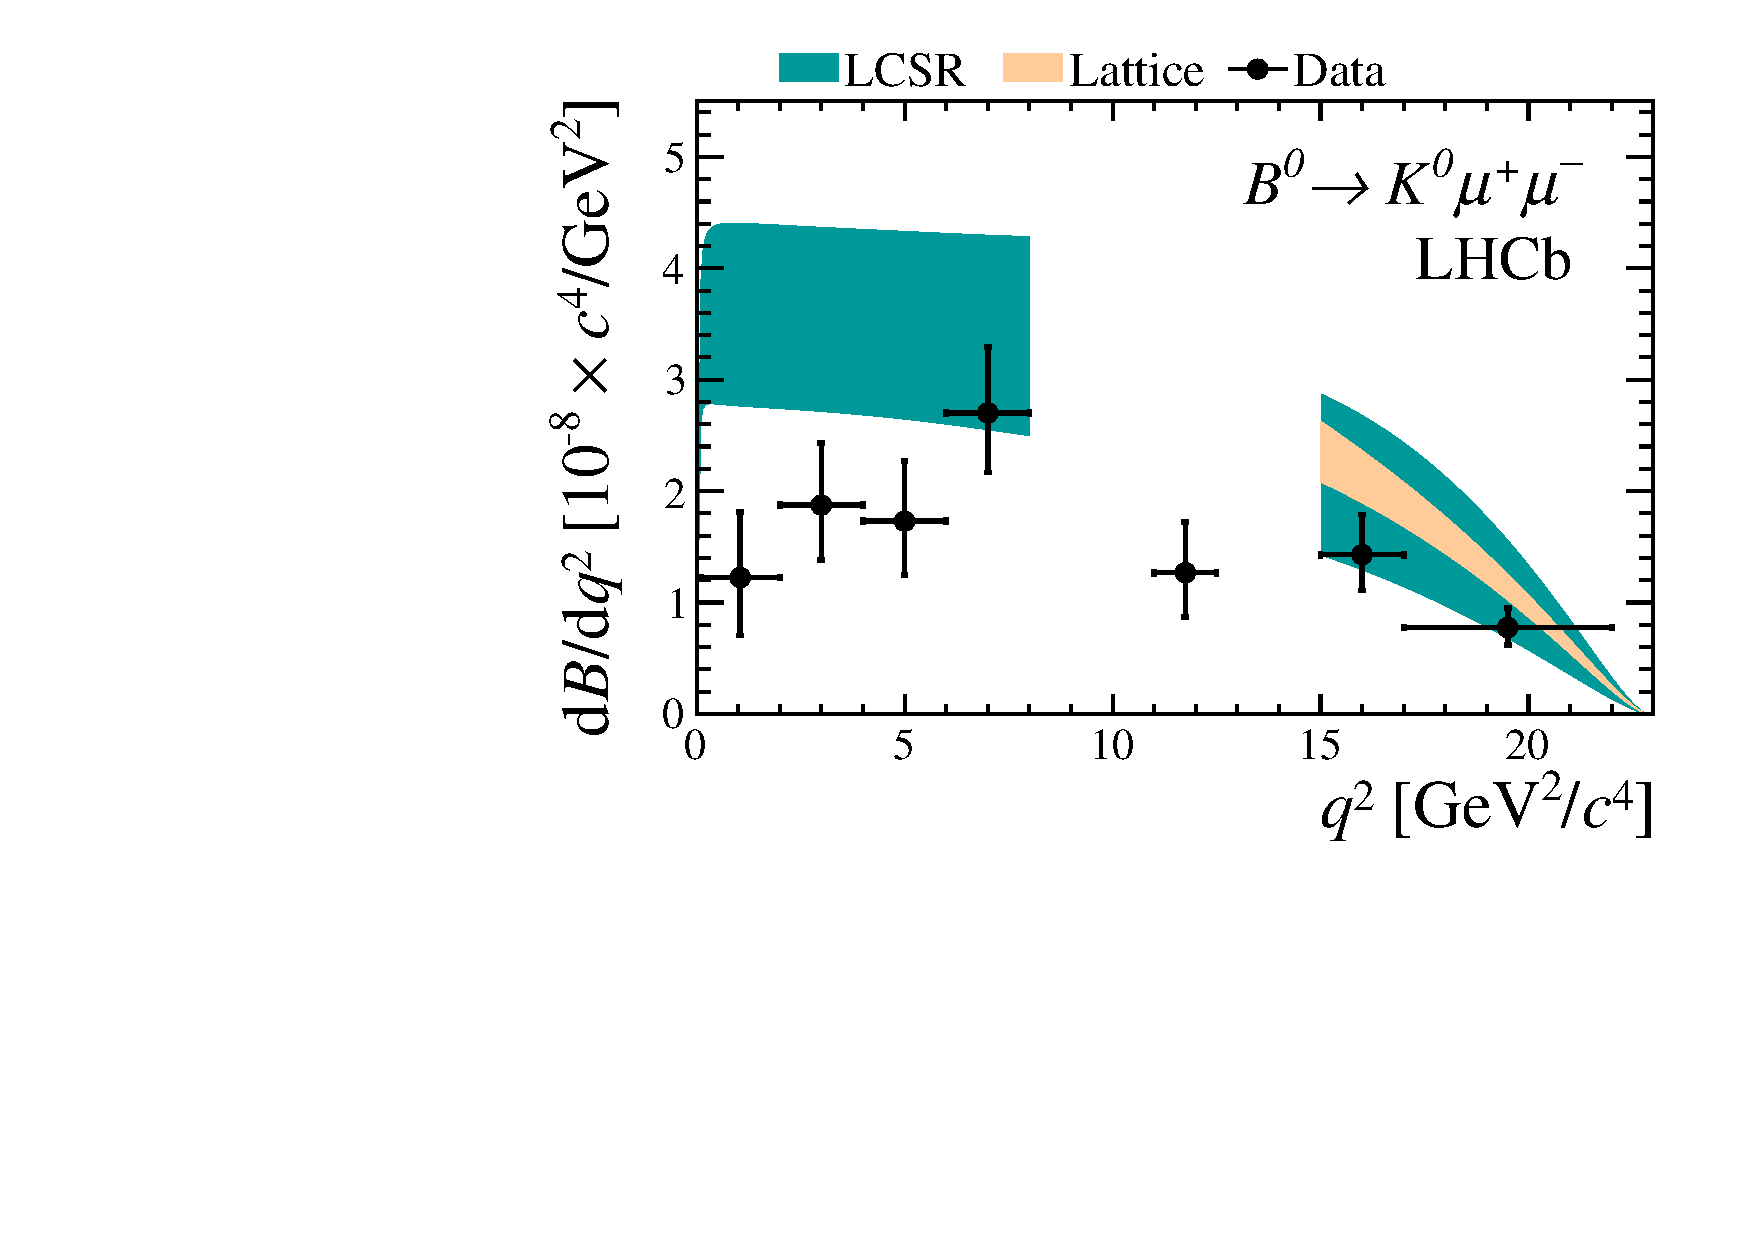
\includegraphics[height=0.33\textheight]{figs/BFs/ksmumu_BF.pdf}};
 \begin{scope}[x={(image.south east)},y={(image.north west)}]
  %\draw[help lines,xstep=.1,ystep=.1] (0,0) grid (1,1);
  %\node[draw=none] at (0.45,0.85) {\tiny \BsTophimm};
 \end{scope}
\end{tikzpicture}
\begin{tikzpicture}
 \centering
 \node[anchor=south west,inner sep=0](image) at (0,0) {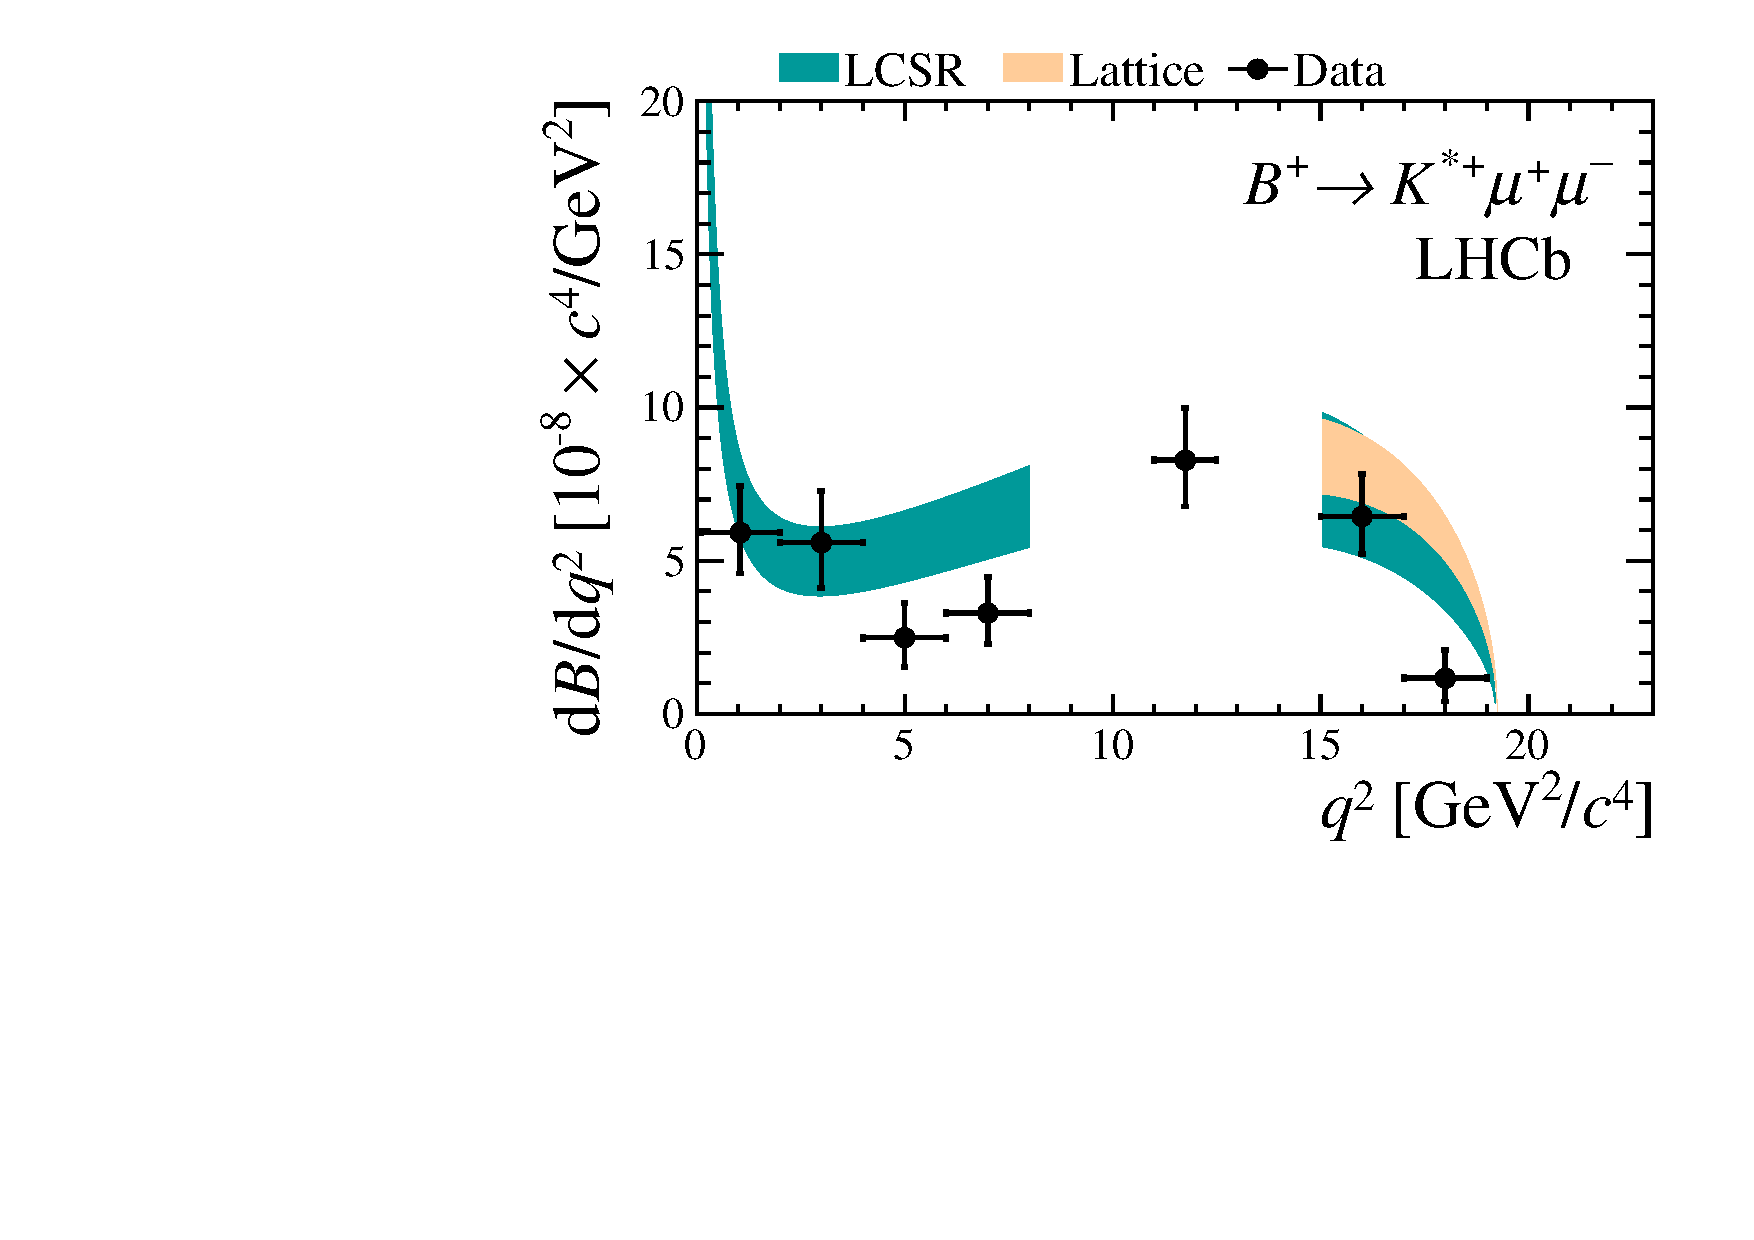
\includegraphics[height=0.33\textheight]{figs/BFs/bukst_BF.pdf}};
 \begin{scope}[x={(image.south east)},y={(image.north west)}]
  %\draw[help lines,xstep=.1,ystep=.1] (0,0) grid (1,1);
  %\node[draw=none] at (0.45,0.85) {\tiny \BsTophimm};
 \end{scope}
\end{tikzpicture}
\end{center}

\end{frame}

%%%%%%%%%%%%%%%%%%%%%%%%%%%%%%%%%%%%%%%%%%%%%%%%%%%%%%%%%%%%%%%%
%Slide
%%%%%%%%%%%%%%%%%%%%%%%%%%%%%%%%%%%%%%%%%%%%%%%%%%%%%%%%%%%%%%%%%
\begin{frame}{Previous measurements: Angular analysis of $\decay{\Bd}{\KstP\mup\mun}$}

\begin{itemize}
\item[$\blacktriangleright$] \KstP is a P-wave (spin-1) state which decays to $\Kp\pim$
\item[$\blacktriangleright$] Decay fully described by $\qsq\equiv m_{\mu\mu}^{2}$ and three angles: $\thetal,\thetak,\phi$
\item[$\blacktriangleright$] Can write an expression for the angular decay distribution 
  \begin{itemize}
    \item[\ding{70}] Depends on the spin of the \Kstar meson
  \end{itemize}
\end{itemize}

  \begin{columns}
   \begin{column}{0.6\textwidth}
  \scalebox{0.8}{\parbox{.5\linewidth}{%
  \begin{align*}
   \frac{1}{\deriv(\Gamma+\bar{\Gamma})/\deriv q^2} & \left. \frac{\deriv^3(\Gamma+\bar{\Gamma})}{\deriv\Omega}\right|_{\rm P-wave} = \\
    \frac{9}{32\pi} \Big[& 
     \tfrac{3}{4} (1-\textcolor{cobalt}{{F_{\rm L}}})\sin^2\thetak + \textcolor{cobalt}{{F_{\rm L}}}\cos^2\thetak\\
     &+ \tfrac{1}{4}(1-\textcolor{cobalt}{{F_{\rm L}}})\sin^2\thetak\cos 2\thetal \\
     &- \textcolor{cobalt}{{F_{\rm L}}} \cos^2\thetak\cos 2\thetal + \textcolor{cobalt}{{S_3}}\sin^2\thetak \sin^2\thetal \cos 2\phi\nonumber\\
     &+ \textcolor{cobalt}{{S_4}} \sin 2\thetak \sin 2\thetal \cos\phi + \textcolor{cobalt}{{S_5}}\sin 2\thetak \sin \thetal \cos \phi\nonumber\\
     &+ \tfrac{4}{3} \textcolor{cobalt}{{A_{\rm FB}}} \sin^2\thetak \cos\thetal + \textcolor{cobalt}{{S_7}} \sin 2\thetak \sin\thetal \sin\phi\nonumber\\
     &+ \textcolor{cobalt}{{S_8}} \sin 2\thetak \sin 2\thetal \sin\phi + \textcolor{cobalt}{{S_9}}\sin^2\thetak \sin^2\thetal \sin 2\phi  \Big]
  \end{align*}
  }}
   \end{column}
   \begin{column}{0.4\textwidth}
    \resizebox{\columnwidth}{!}{
    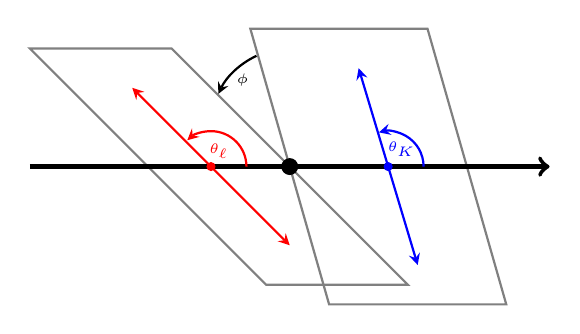
\begin{tikzpicture}
    %\draw[step=1cm,gray,very thin] (0,0) grid (7,4);
    %planes
    \draw[thick,gray] (0.2,3.5)--(2,3.5)--(5,0.5)--(3.2,0.5)--cycle;
    \draw[thick,gray] (3.,3.75)--(4.,0.25)--(6.25,0.25)--(5.25,3.75)--cycle;
    %axis
    \draw[ultra thick,->] (0.2,2.0) -- (6.8,2.0);
    %B
    \draw[fill] (3.5,2) circle (0.1);
    \node[draw=none] at (3.7,2.3){\tiny \Bz};
    %mumu
    \draw[fill,red] (2.5,2) circle (0.05);
    \draw[thick,->,red,>=stealth] (2.5,2) -- (1.5,3);
    \draw[thick,->,red,>=stealth] (2.5,2) -- (3.5,1);
    \node[draw=none,red] at (1.5,2.65){\tiny \mup};
    \node[draw=none,red] at (3.1,1.1){\tiny \mun};
    \draw[thick,red,->,>=stealth] ([shift=(0:0.45)]2.5,2) arc (0:132:0.45);
    \node[draw=none,red] at (2.6,2.2){\tiny $\theta_{\ell}$};

    %kpi
    \draw[fill,blue] (4.75,2) circle (0.05);
    \draw[thick,->,blue,>=stealth] (4.75,2) -- (4.375,3.25);
    \draw[thick,->,blue,>=stealth] (4.75,2) -- (5.125,0.75);
    \node[draw=none,blue] at (4.85,2.95){\tiny \Kp};
    \node[draw=none,blue] at (5.30,1.3){\tiny \pim};
    \draw[thick,blue,->,>=stealth] ([shift=(0:0.45)]4.75,2) arc (0:105:0.45);
    \node[draw=none,blue] at (4.92,2.22){\tiny $\theta_{K}$};

    \draw[thick,->,>=stealth] ([shift=(115:1.)]3.5,2.5) arc (115:155:1.);
    \node[draw=none] at (2.9,3.1){\tiny $\phi$};
    \end{tikzpicture}
    }
   \end{column}
  \end{columns}

  \begin{itemize}
  \item[$\blacktriangleright$] $\textcolor{cobalt}{{F_{\rm L}}}$, $\textcolor{cobalt}{{A_{\rm FB}}}$, $\textcolor{cobalt}{{S_i}}$ are the angular observables which are measured
  \begin{itemize}
    \item[\ding{70}] Can be compared with SM predictions
    \end{itemize}
  \item[$\blacktriangleright$] Often useful to measure ratios of observables e.g. $P'_{4,5} = \textcolor{cobalt}{S_{4,5}}/\sqrt{ \textcolor{cobalt}{F_{\rm L}}(1 -  \textcolor{cobalt}{F_{\rm L}})}$
%    \begin{itemize}
%    \item[\ding{70}] 
%    \end{itemize}
  \end{itemize}
\end{frame}

%%%%%%%%%%%%%%%%%%%%%%%%%%%%%%%%%%%%%%%%%%%%%%%%%%%%%%%%%%%%%%%%
%Slide
%%%%%%%%%%%%%%%%%%%%%%%%%%%%%%%%%%%%%%%%%%%%%%%%%%%%%%%%%%%%%%%%%
\begin{frame}{Previous measurements: Angular analysis of \BdToKstmmP}

\begin{itemize}
    \item[\ding{72}] Deviations in $P'_{5}$ at level of 2.9$\sigma$ in two \qsq bins
\end{itemize}

\begin{center}
\begin{tikzpicture}
    \centering
    \node[anchor=south west,inner sep=0](image) at (0,0) {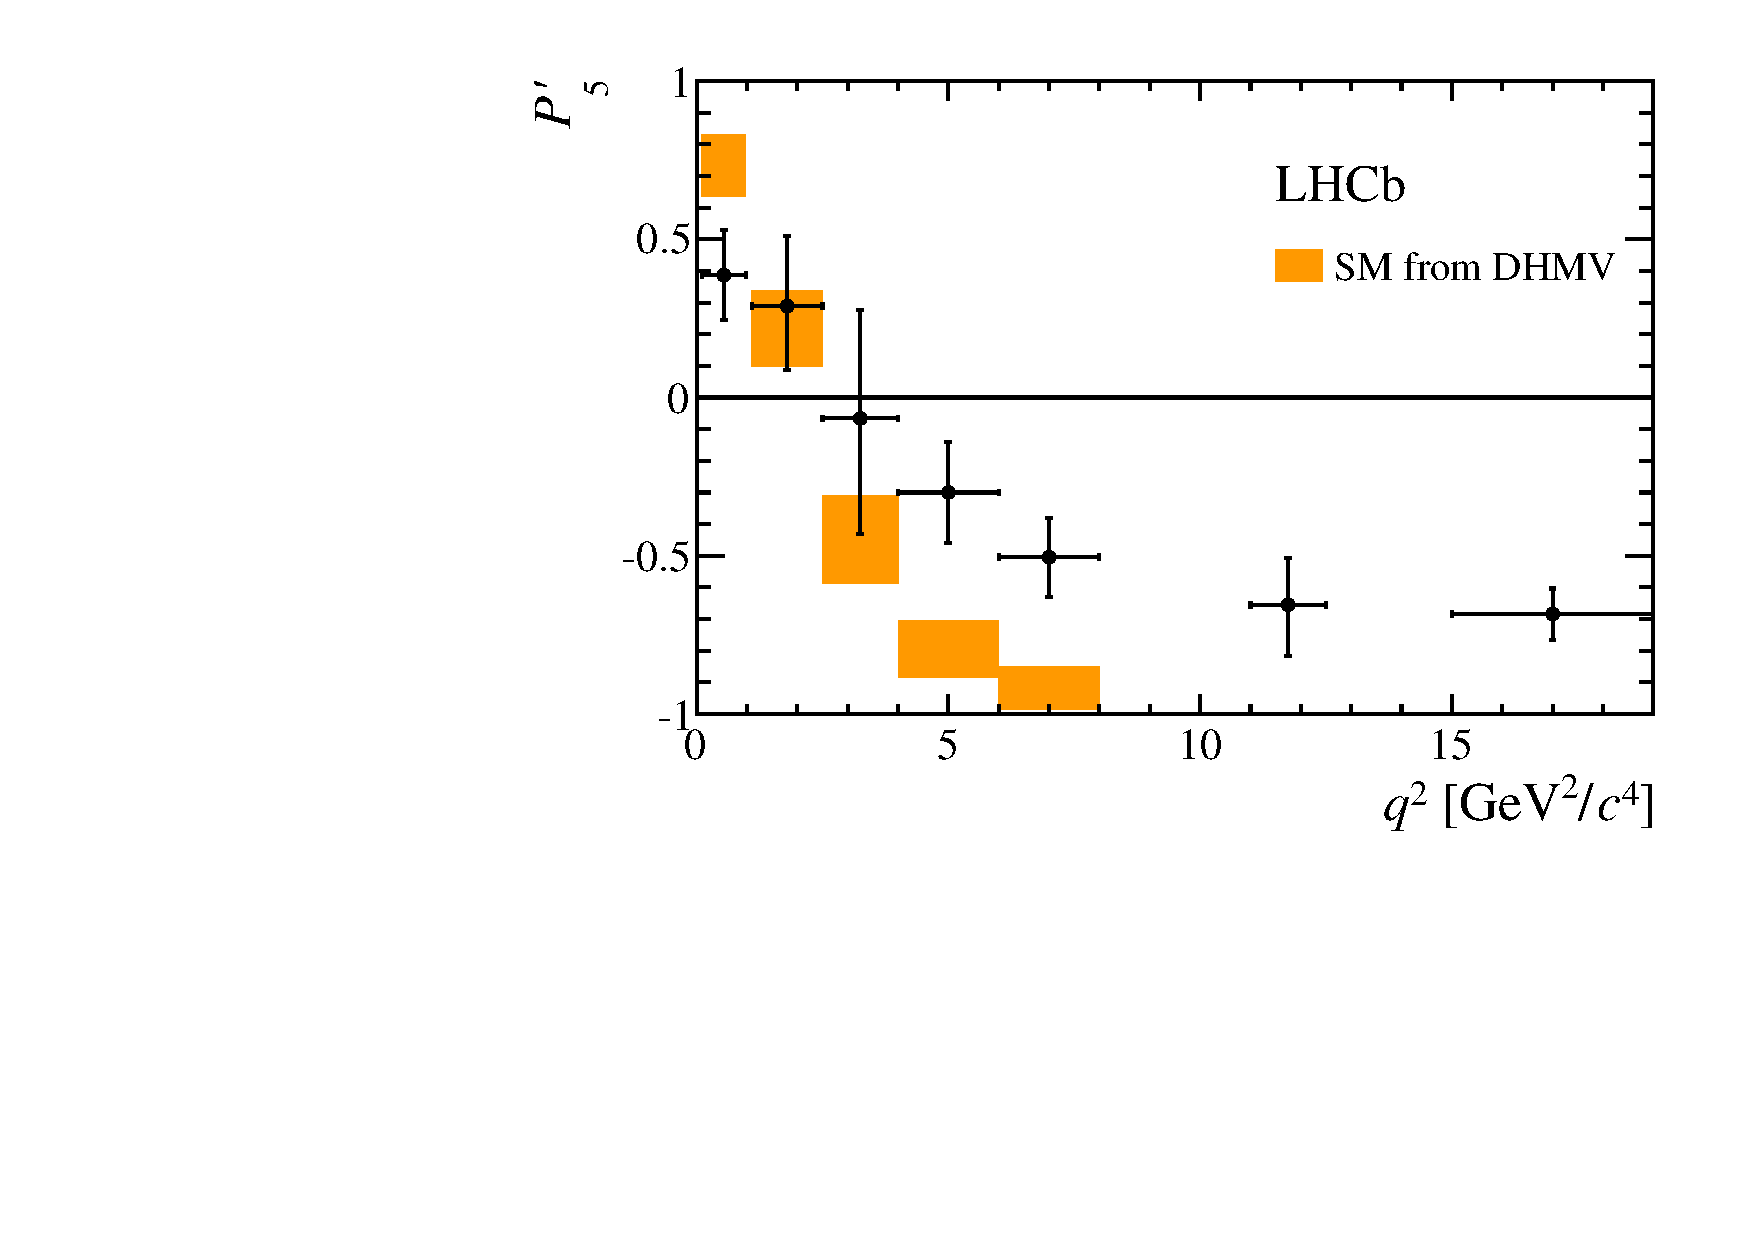
\includegraphics[width=0.5\textwidth]{figs/kpimm/introduction/P5prime.pdf}};
    \begin{scope}[x={(image.south east)},y={(image.north west)}]
      %\draw[help lines,xstep=.1,ystep=.1] (0,0) grid (1,1);
      \node[draw,ellipse,darkpastelred,minimum width=40pt,minimum height=50pt,thick,dashed] at (0.41,0.35) {};
      %\node[draw=none] at (0.4,0.875) {\tiny [JHEP 02 (2016) 104]};
    \end{scope}
  \end{tikzpicture}
\end{center}

\begin{itemize}
  \item[$\blacktriangleright$] Results form a {\bf consistent pattern} with the deviations in $\deriv\BF/\deriv\qsq$ measurements
  \item[$\blacktriangleright$] Two possible interpretations that can explain this pattern are:
  \begin{itemize}
    \item[\ding{182}] Contribution of NP, e.g. a new vector Z' boson
    \item[\ding{183}] Underestimation of effects of the strong force
  \end{itemize}
\end{itemize}
\end{frame}

%%%%%%%%%%%%%%%%%%%%%%%%%%%%%%%%%%%%%%%%%%%%%%%%%%%%%%%%%%%%%%%%%
%Slide
%%%%%%%%%%%%%%%%%%%%%%%%%%%%%%%%%%%%%%%%%%%%%%%%%%%%%%%%%%%%%%%%%
\begin{frame}{\BdToKpimm in the \Kstarfourteenthirty region \hspace{0pt plus 1 filll} {\small \bf \textcolor{black}{[JHEP 12 (2016) 065]}}}

\begin{itemize}
\item[$\blacktriangleright$] Analyses of \BdToKpimm at \lhcb have focused on the (P-wave) \KstarP
\item[$\blacktriangleright$] Region of \mkpi $\sim$1430\mevcc contains contributions from S-, P- and D-wave $K^\ast$ states (spin-0,1,2)
\begin{itemize}
  \item[\ding{70}] Leads to a very complicated angular expression!
\end{itemize}
\end{itemize}

\begin{center}
\begin{tikzpicture}
 \node[anchor=south west,inner sep=0](image) at (0,0) {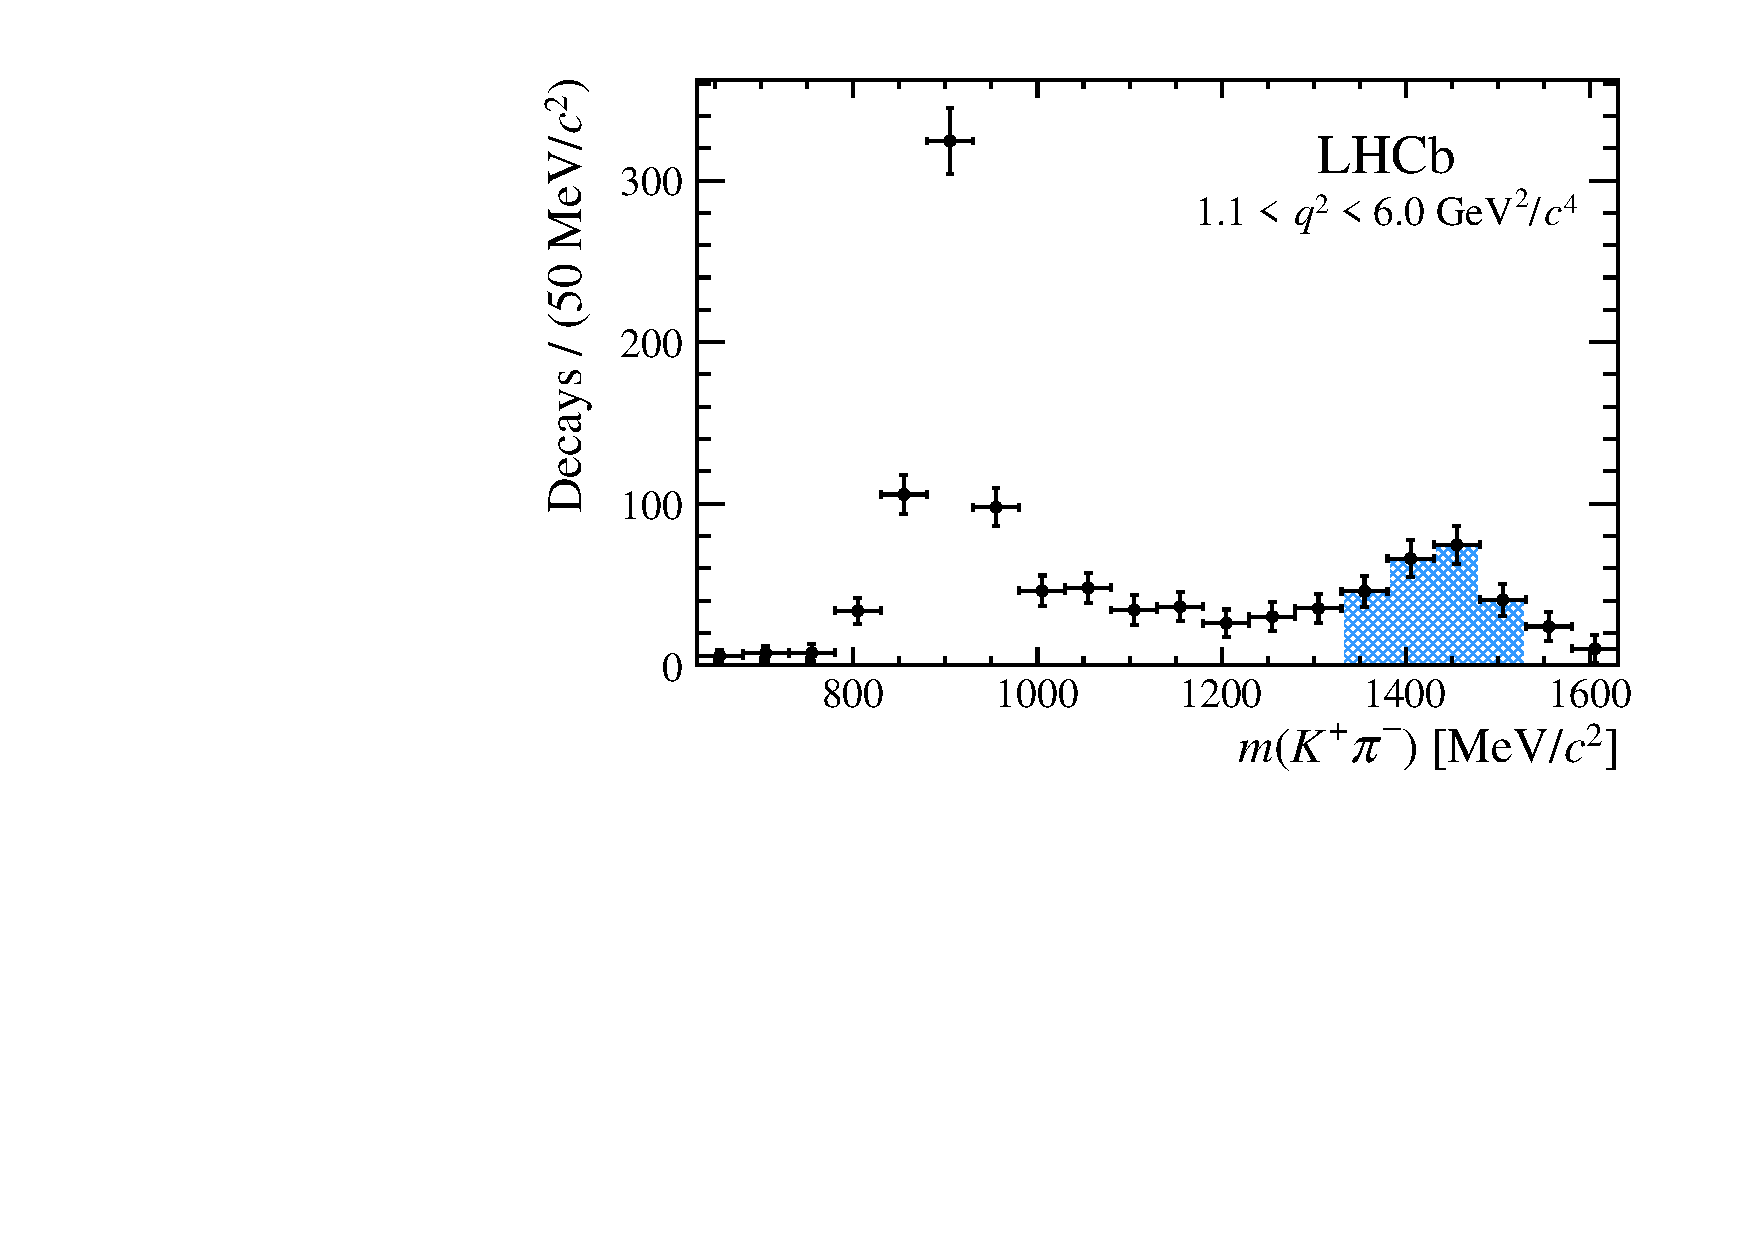
\includegraphics[width=0.5\textwidth]{figs/kpimm/introduction/full-mkpi.pdf}};
 \begin{scope}[x={(image.south east)},y={(image.north west)}]
  %\draw[help lines,xstep=.1,ystep=.1] (0,0) grid (1,1);
  \node[draw=none] at (0.25,0.75) {\footnotesize \color{red}{\KstarP}};
  \draw[->,thick,red] (0.25, 0.7) -- (0.35,0.4);
  \node[draw=none] at (0.75,0.6) {\footnotesize \color{blue}{New region}};
  \draw[->,thick,blue] (0.75, 0.55) -- (0.78,0.37);
 \end{scope}
\end{tikzpicture}
\end{center}

\begin{itemize}
  \item[$\blacktriangleright$] Will present the first measurements of the differential branching fraction and angular analysis in this new \mkpi region
\end{itemize}

\end{frame}

%%%%%%%%%%%%%%%%%%%%%%%%%%%%%%%%%%%%%%%%%%%%%%%%%%%%%%%%%%%%%%%%%
%Slide
%%%%%%%%%%%%%%%%%%%%%%%%%%%%%%%%%%%%%%%%%%%%%%%%%%%%%%%%%%%%%%%%%
\begin{frame}{Signal extraction}

\begin{itemize}
  \item[$\blacktriangleright$] Fit to invariant mass distribution required to separate the signal from background contributions
  %\item Signal modelled with sum of two Gaussians with power-law tail on the low-mass side
  %\item Combinatorial background is modelled using an exponential function
  \item[$\blacktriangleright$] $\sim230$ signal candidates in $1.1<\qsq<6.0\gevgevcccc$
\end{itemize}

\begin{center}
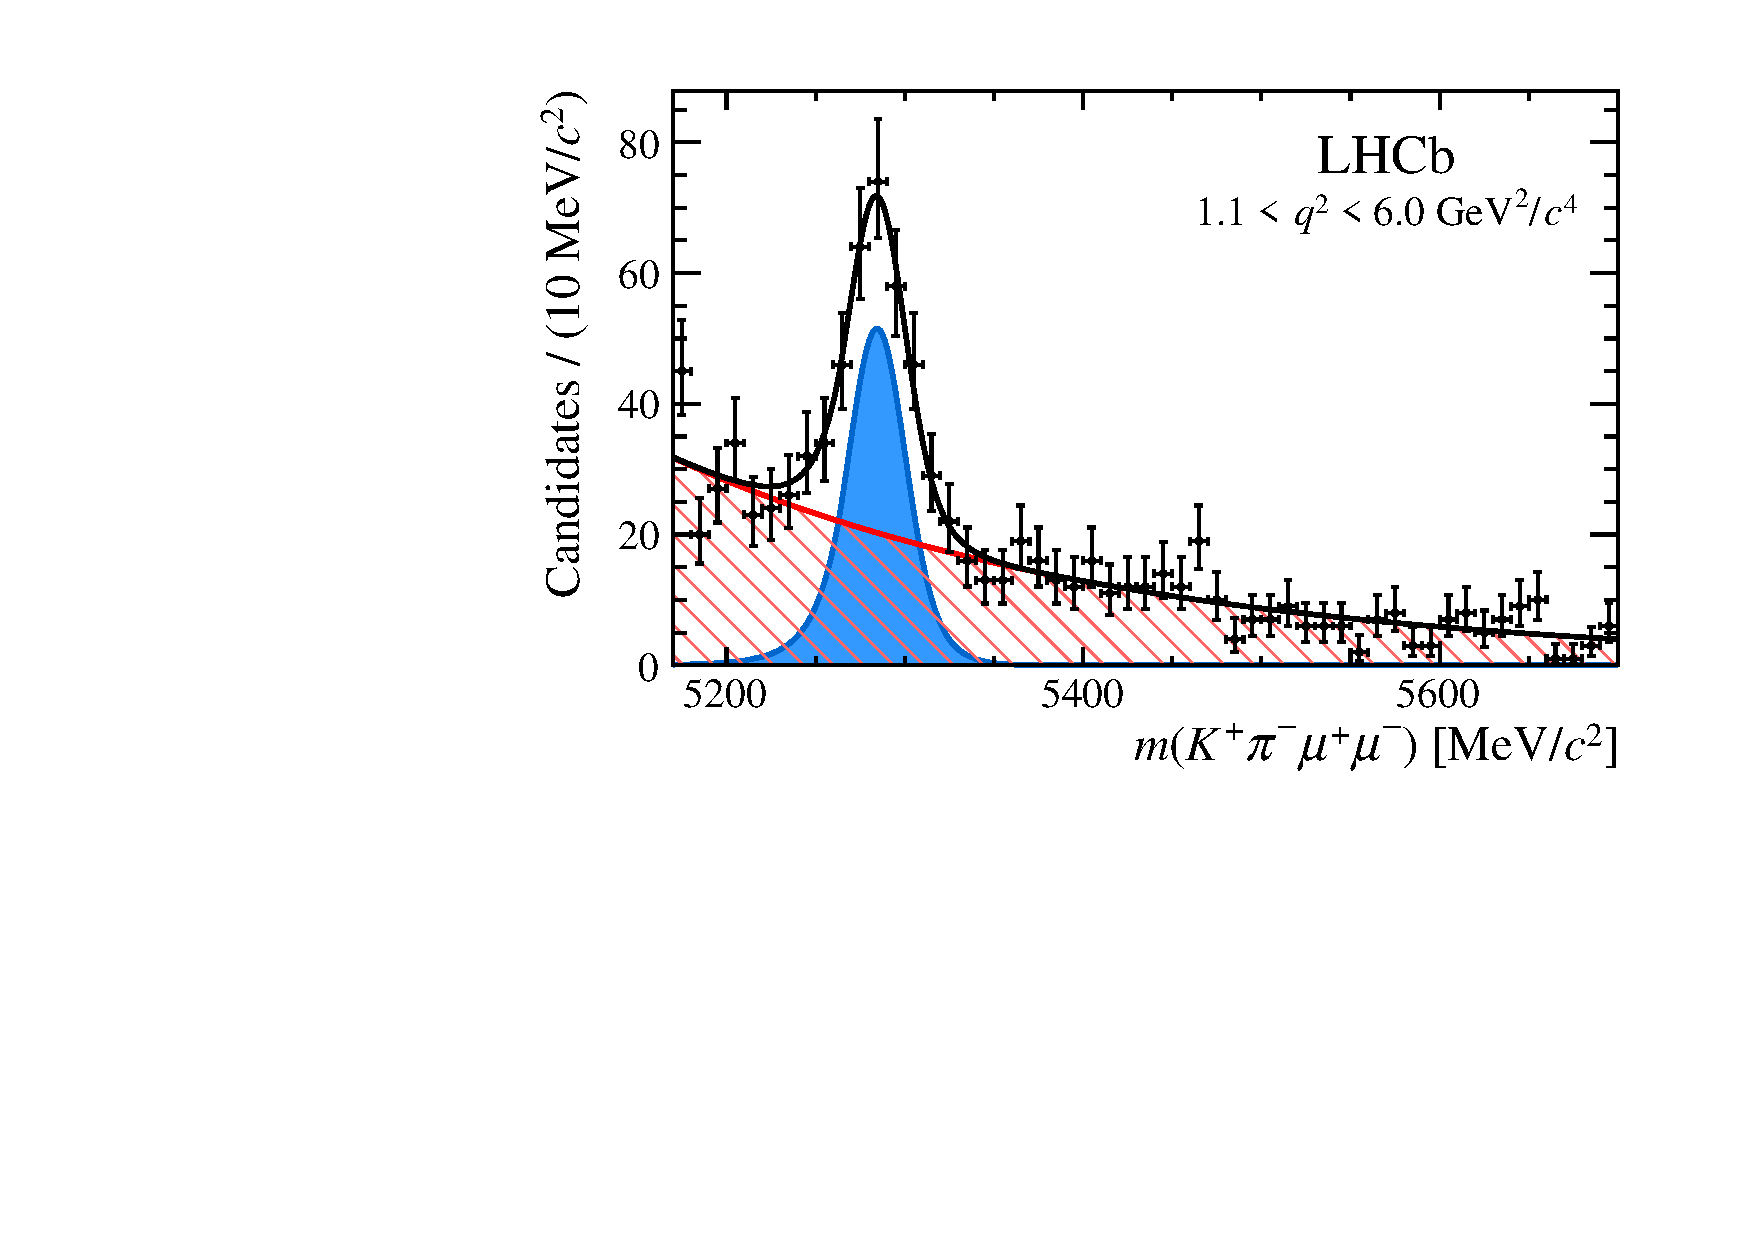
\includegraphics[width=0.6\textwidth]{figs/kpimm/massfit/fitKpimumu_q2_1p1_6p0.pdf}
\end{center}

\end{frame}

%%%%%%%%%%%%%%%%%%%%%%%%%%%%%%%%%%%%%%%%%%%%%%%%%%%%%%%%%%%%%%%%%
%Slide
%%%%%%%%%%%%%%%%%%%%%%%%%%%%%%%%%%%%%%%%%%%%%%%%%%%%%%%%%%%%%%%%%
\begin{frame}{Efficiency studies}

\begin{itemize}
  \item[$\blacktriangleright$] The selection efficiency of the signal candidates varies as a function of the decay angles $\thetal,\thetak,\phi$
  \item[$\blacktriangleright$] In order to perform an angular analysis, need to carefully understand this effect
  \item[$\blacktriangleright$] In this analysis, the efficiency distribution is modelled using a Legendre polynomial parameterisation
  %\begin{itemize}
  %  \item Requires 1764 legendre coefficients!
  %\end{itemize}
\end{itemize}

\bigskip

\begin{center}
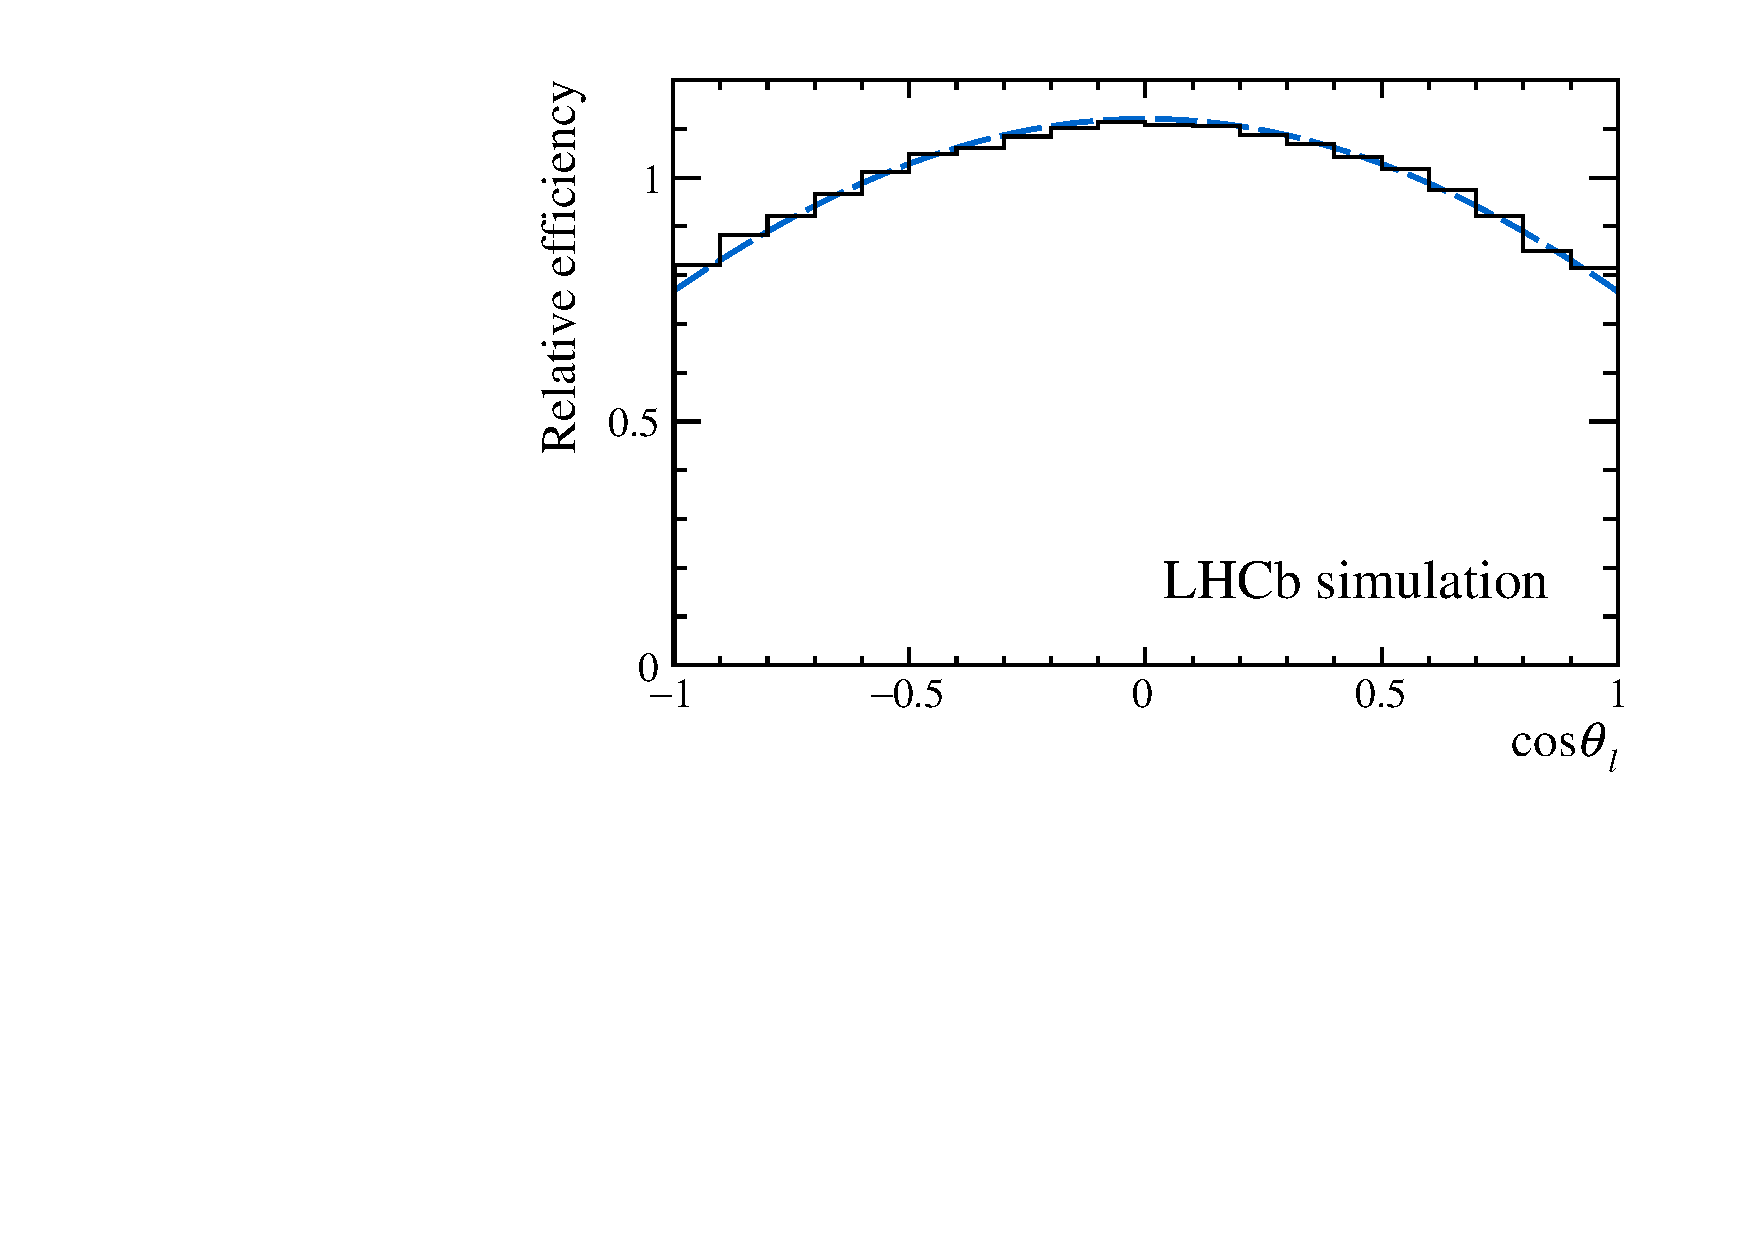
\includegraphics[width=0.32\textwidth]{figs/kpimm/acceptance/Fig3a.pdf}
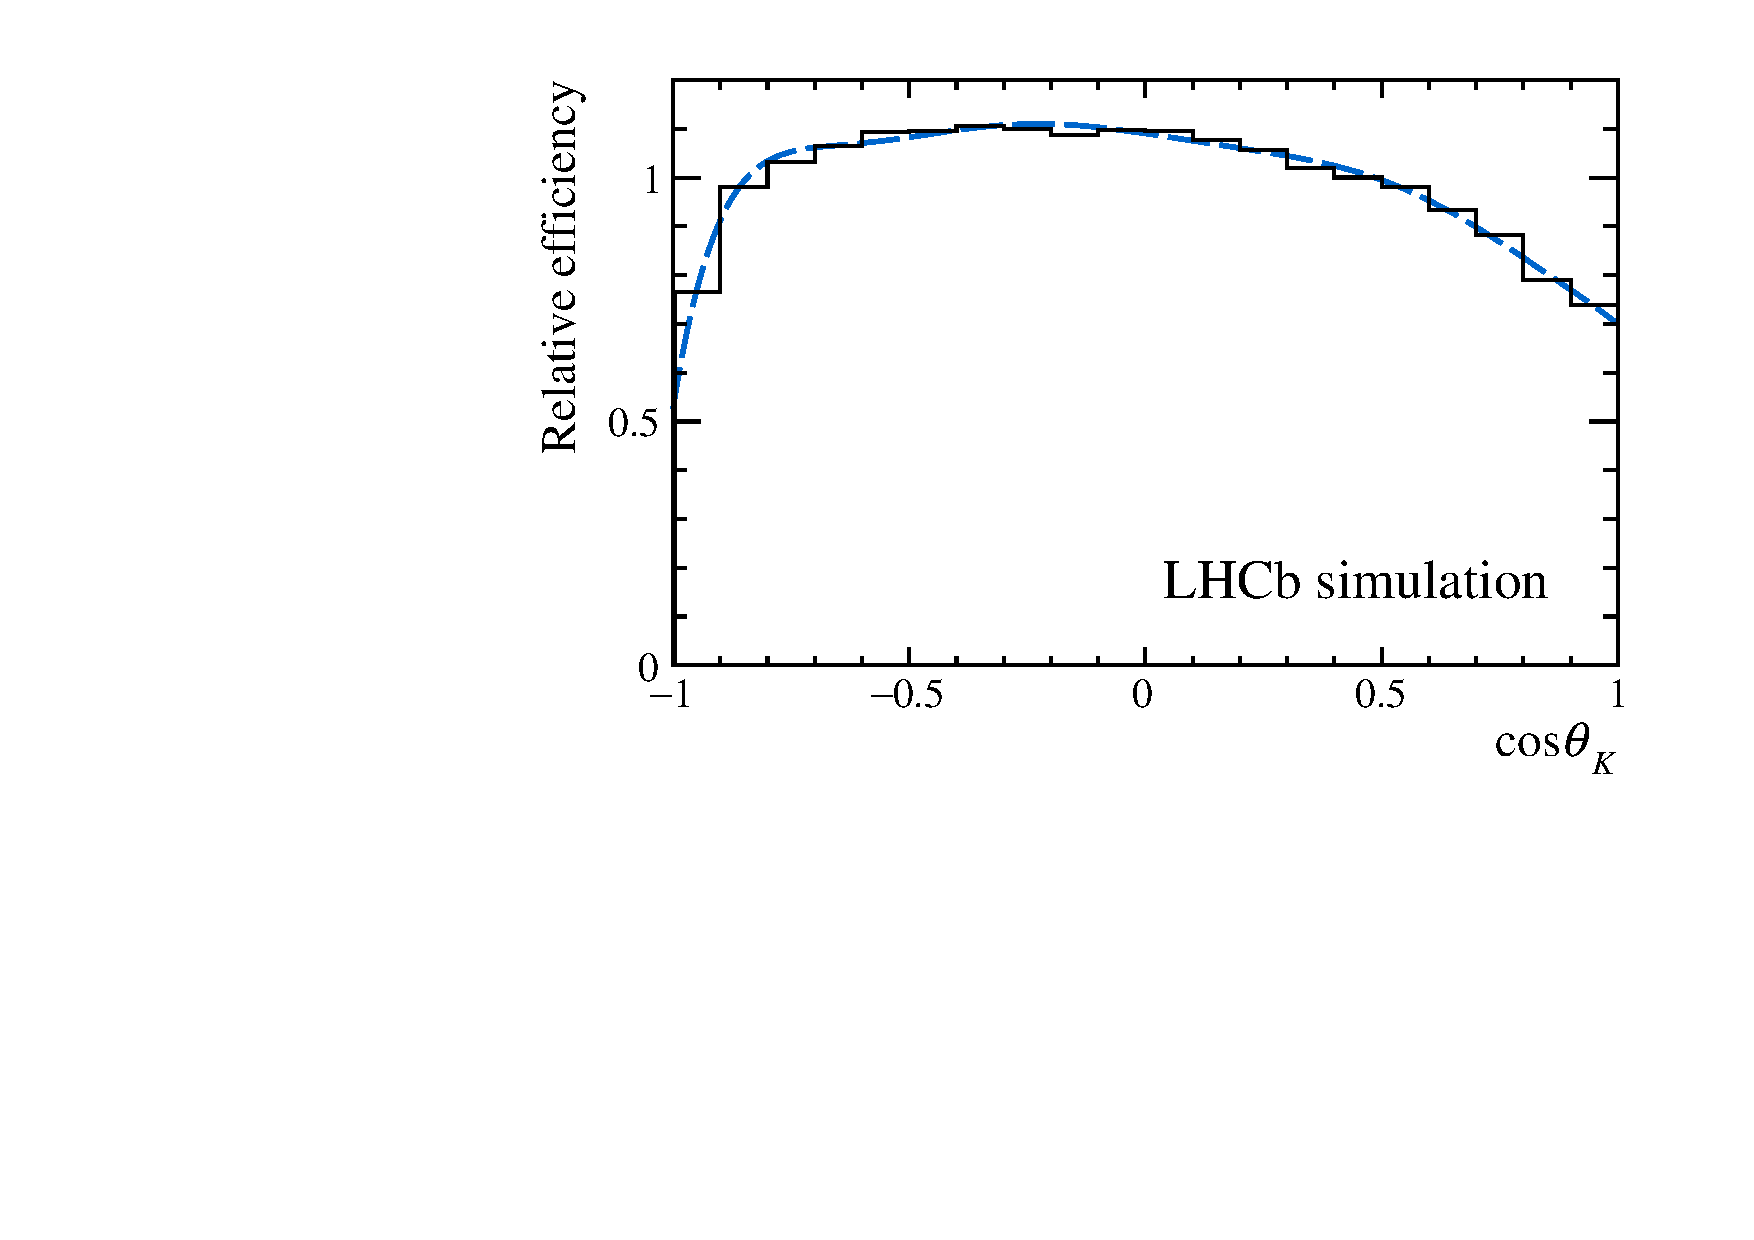
\includegraphics[width=0.32\textwidth]{figs/kpimm/acceptance/Fig3b.pdf}
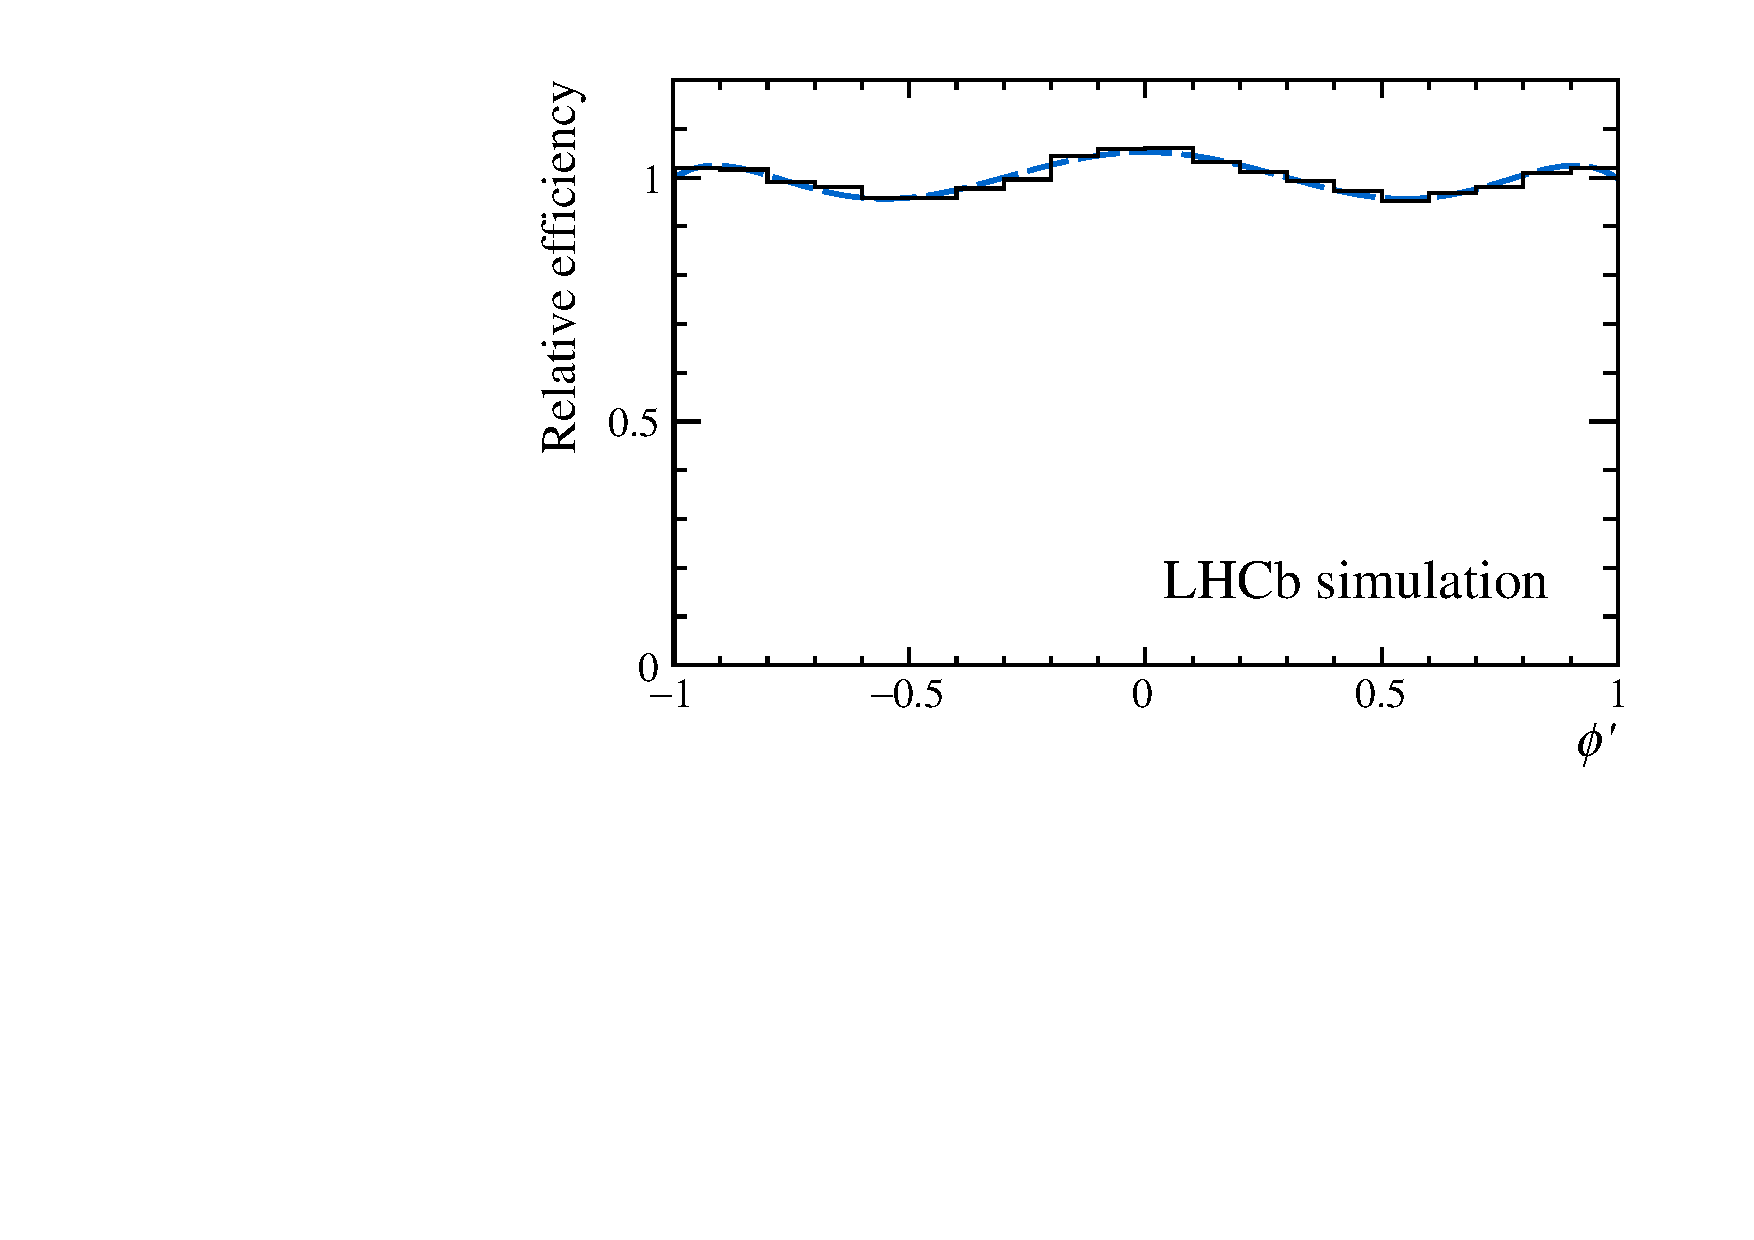
\includegraphics[width=0.32\textwidth]{figs/kpimm/acceptance/Fig3c.pdf}
\end{center}

\end{frame}

%%%%%%%%%%%%%%%%%%%%%%%%%%%%%%%%%%%%%%%%%%%%%%%%%%%%%%%%%%%%%%%%%
%Slide
%%%%%%%%%%%%%%%%%%%%%%%%%%%%%%%%%%%%%%%%%%%%%%%%%%%%%%%%%%%%%%%%%
\begin{frame}{Differential branching fraction ($\deriv\BF/\deriv\qsq$)}

\begin{itemize}
\item[$\blacktriangleright$] {\bf First} $\deriv\BF/\deriv\qsq$ measurement of \BdToKpimm in this region of \mkpi 
\end{itemize}

\begin{center}
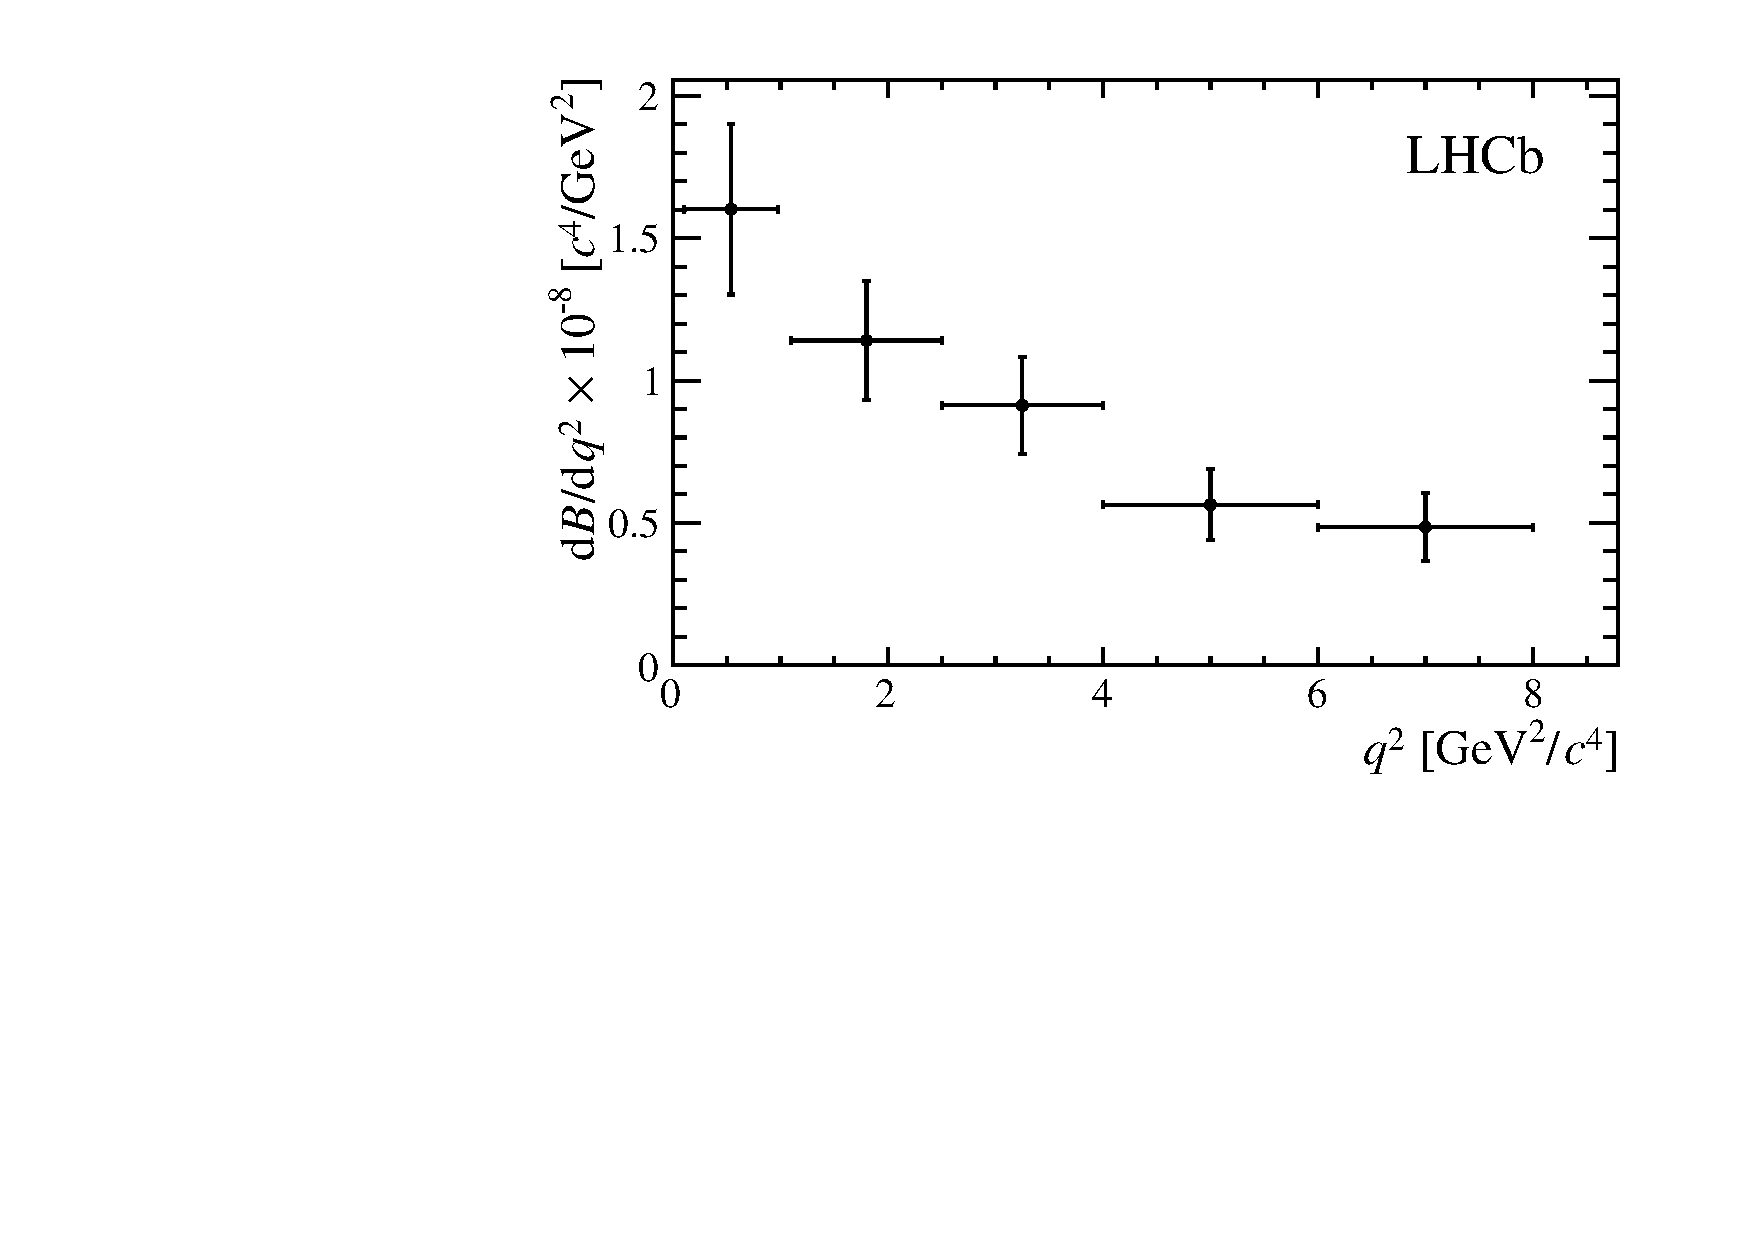
\includegraphics[width=0.6\textwidth]{figs/kpimm/bf/dbfdq2.pdf}
\end{center}

\begin{itemize}
\item[$\blacktriangleright$] Currently no SM predictions
\begin{itemize}
\item[\ding{72}] Hope this measurement stimulates further theory effort in this area
\end{itemize}
\end{itemize}

\end{frame}

%%%%%%%%%%%%%%%%%%%%%%%%%%%%%%%%%%%%%%%%%%%%%%%%%%%%%%%%%%%%%%%%%
%Slide
%%%%%%%%%%%%%%%%%%%%%%%%%%%%%%%%%%%%%%%%%%%%%%%%%%%%%%%%%%%%%%%%%
\begin{frame}{Angular analysis}

\begin{itemize}
\item[$\blacktriangleright$] Angular distribution for \BdToKpimm decays encompassing S-, P- and D-wave \Kstar states can be expressed in an orthonormal basis of angular functions, $f_i(\thetal,\thetak,\phi)$,
\begin{equation*}
\frac{\deriv\Gamma }{\deriv\qsq\,\deriv\Omega} \propto \sum^{41}_{i=1} f_i (\thetal,\thetak,\phi) \Gamma_i(\qsq)
%\quad\mbox{with}\quad
%\int f_if_j\deriv\costhetal\deriv\costhetak\deriv\phi = \delta_{ij}
\end{equation*}
\item[$\blacktriangleright$] 41 angular terms compared to 11 for \BdToKstmmP!
\item[$\blacktriangleright$] Define 40 normalised angular moments which form the set of observables that are measured
\end{itemize}
\begin{equation*}
\overline{\Gamma}_i(\qsq) = \frac{\Gamma_{i}(\qsq)}{\Gamma_{1}(\qsq)}
\end{equation*}

\end{frame}

%%%%%%%%%%%%%%%%%%%%%%%%%%%%%%%%%%%%%%%%%%%%%%%%%%%%%%%%%%%%%%%%%
%Slide
%%%%%%%%%%%%%%%%%%%%%%%%%%%%%%%%%%%%%%%%%%%%%%%%%%%%%%%%%%%%%%%%%
\begin{frame}{Angular analysis}

\begin{itemize}
  \item[$\blacktriangleright$] Observables measured using an angular moments analysis
  \begin{itemize}
    \item[\ding{70}] Likelihood fit impossible due to complicated angular expression and limited statistics
  \end{itemize}
\end{itemize}

\begin{itemize}
\item[$\blacktriangleright$] Calculate background-subtracted and acceptance-corrected moments
\end{itemize}

\begin{columns}
\begin{column}{0.6\textwidth}
\begin{equation*}
  \begin{aligned}
  \Gamma_i =&  \sum_{k=1}^{n_{\rm sig}} w_{k}f_i(\Omega_k)  - x\sum_{k=1}^{n_{\rm bkg}} w_{k}f_i(\Omega_k)\\
  C_{ij} =& \sum_{k=1}^{n_{\rm sig}} w^{2}_{k}f_i(\Omega_k)f_j(\Omega_k)   + x^2\sum_{k=1}^{n_{\rm bkg}} w^{2}_{k}f_i(\Omega_k)f_j(\Omega_k)
  \end{aligned}
  \label{eqn:mom:sigbkgacc}
\end{equation*}
\end{column}
\begin{column}{0.4\textwidth}
\begin{centering}
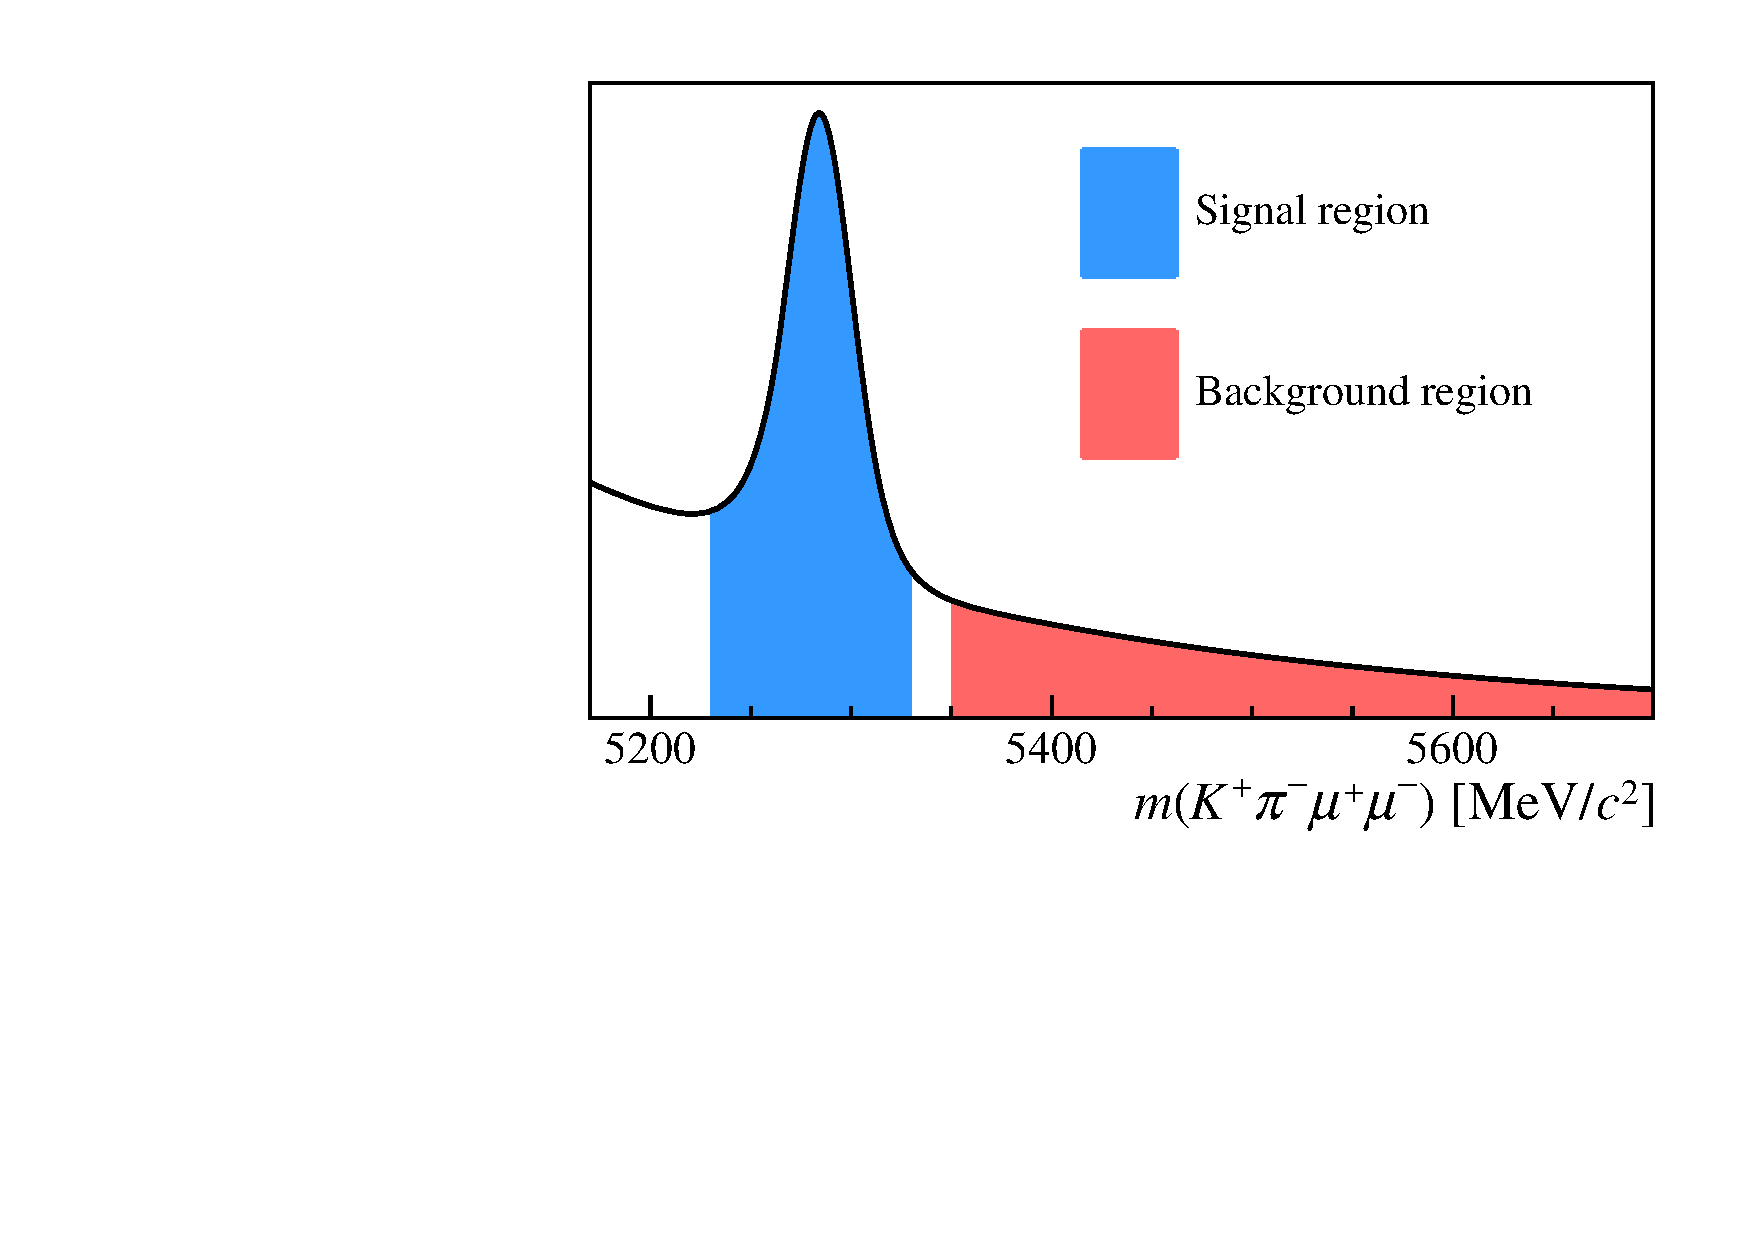
\includegraphics[width=\textwidth]{figs/moments-regions.pdf}
\end{centering}
\end{column}
\end{columns}

\bigskip

\begin{itemize}
\item[$\blacktriangleright$] $x$ is the ratio $\tilde{n}^{\rm bkg}_{\rm sig}/n_{\rm bkg}$ used to perform the background subtraction
\item[$\blacktriangleright$] $w_{k}$ is the reciprocal of the efficiency, $1/\varepsilon_{k}$
\end{itemize}

\end{frame}

%%%%%%%%%%%%%%%%%%%%%%%%%%%%%%%%%%%%%%%%%%%%%%%%%%%%%%%%%%%%%%%%%
%Slide
%%%%%%%%%%%%%%%%%%%%%%%%%%%%%%%%%%%%%%%%%%%%%%%%%%%%%%%%%%%%%%%%%
\begin{frame}{Angular analysis}
\begin{columns}
\begin{column}{0.55\textwidth}
\begin{itemize}
  \item[$\blacktriangleright$] Currently no SM predictions for the angular moments 
  \begin{itemize}
    \item[\ding{72}] Hope measurement will stimulate futher theory effort
  \end{itemize}
\end{itemize}
\begin{itemize}
  \item[$\blacktriangleright$] Results point towards large interference between S- and P-wave states 
  \item[$\blacktriangleright$] Hints of suppressed D-wave contribution% than expected
%  \begin{itemize}
    %\item $F_{\rm D} <$ 0.29 @ 95\% C.L.
%    \item Low w.r.t expectation from previous similar measurement in \decay{\Bd}{\jpsi(\to\mumu) \Kp\pim}
%\end{itemize}
\end{itemize}
\end{column}
\begin{column}{0.45\textwidth}
\centering
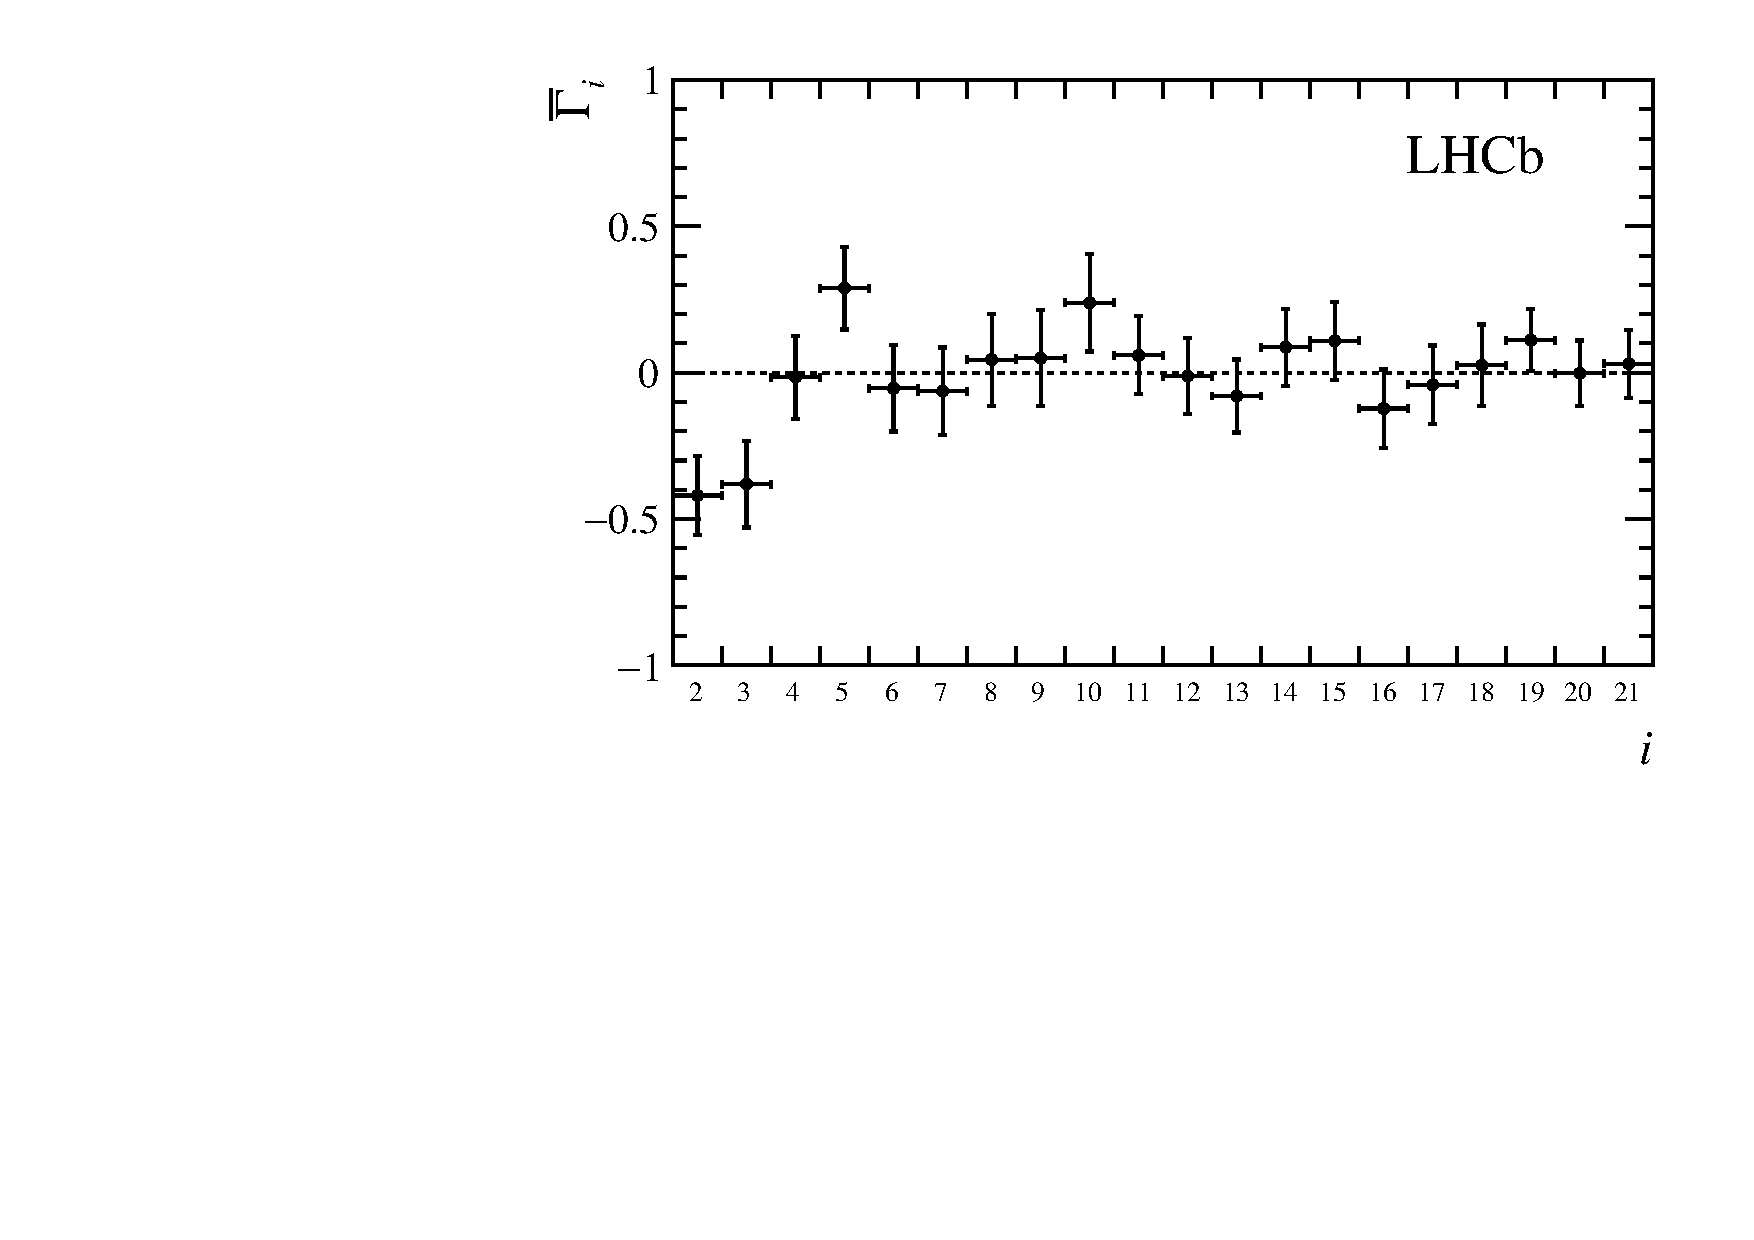
\includegraphics[height=0.44\textheight]{figs/kpimm/angular-analysis/mom_results_2_21.pdf}\\
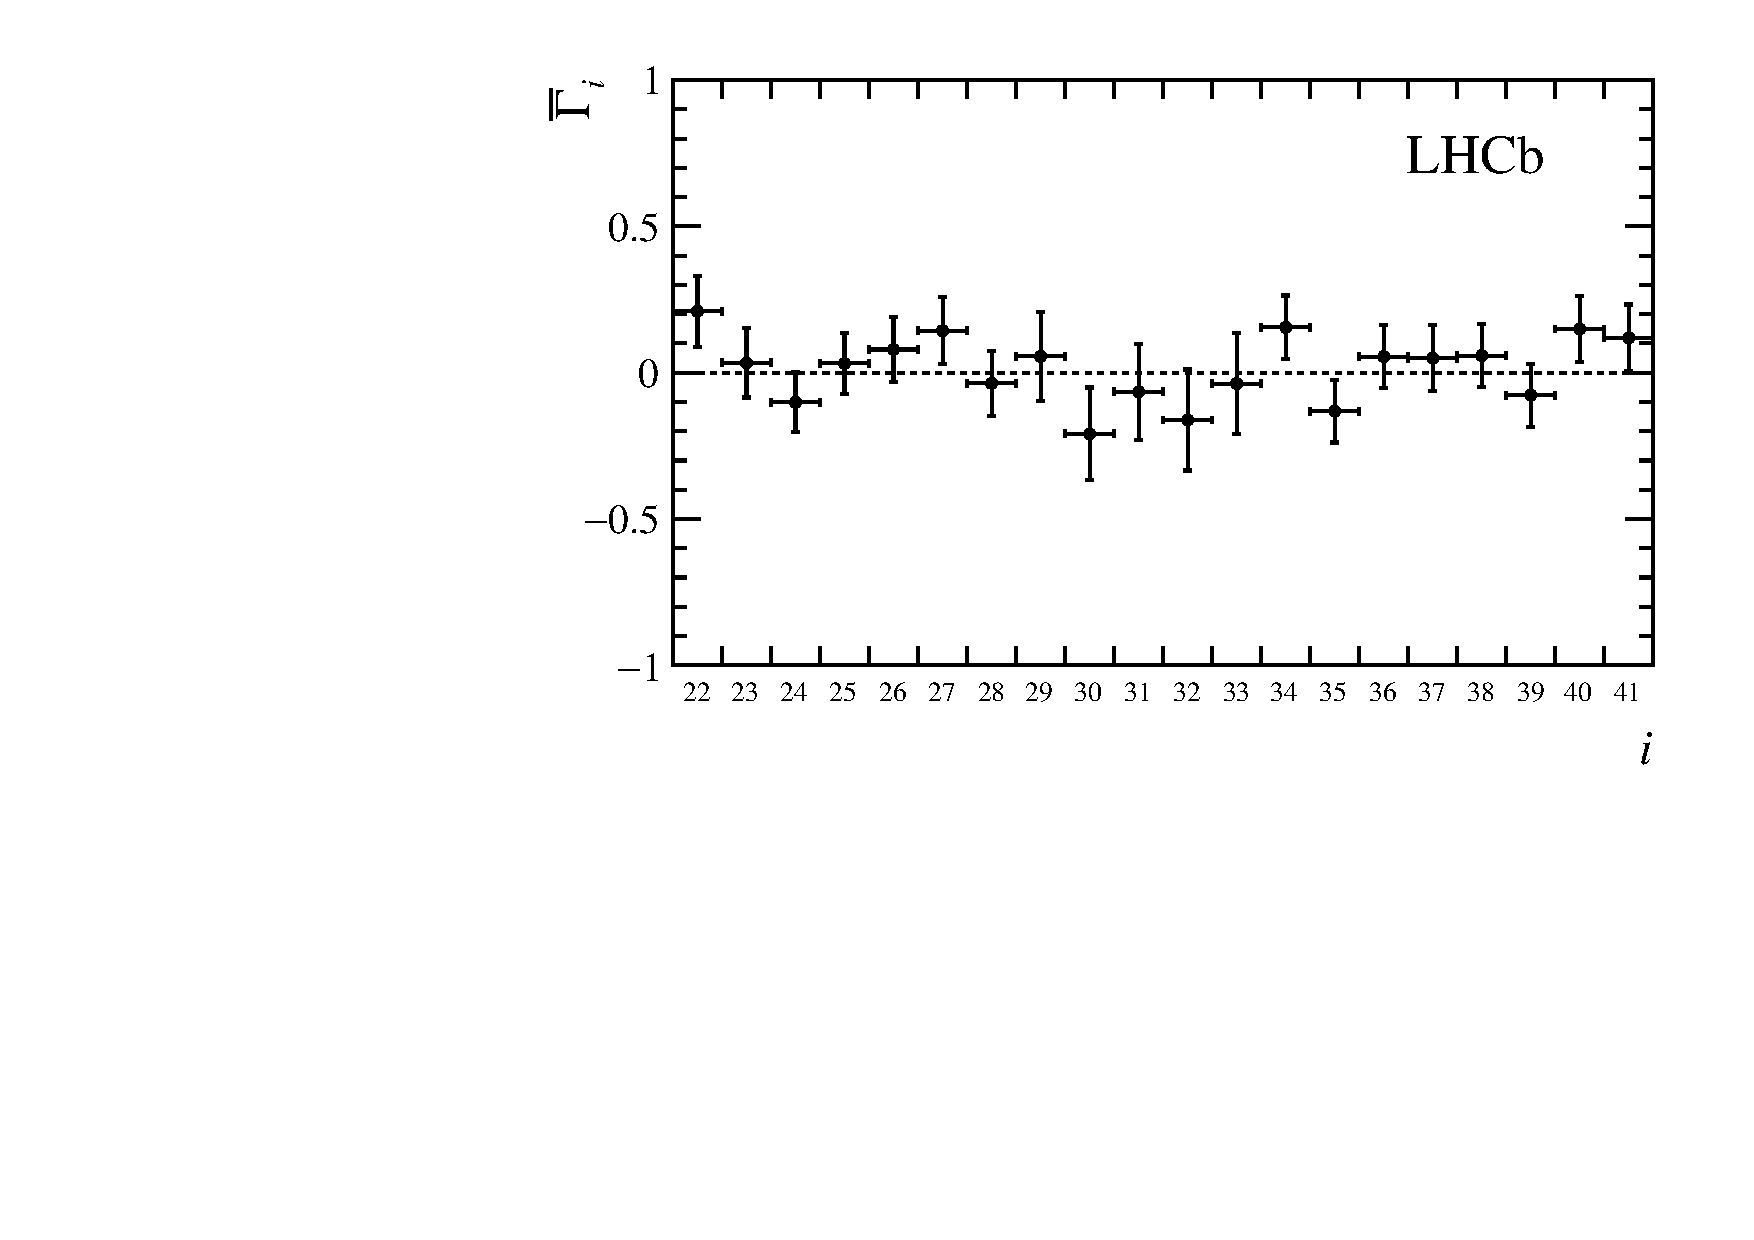
\includegraphics[height=0.44\textheight]{figs/kpimm/angular-analysis/mom_results_22_41.pdf}
\end{column}
\end{columns}
\end{frame}

%%%%%%%%%%%%%%%%%%%%%%%%%%%%%%%%%%%%%%%%%%%%%%%%%%%%%%%%%%%%%%%%%
%Slide
%%%%%%%%%%%%%%%%%%%%%%%%%%%%%%%%%%%%%%%%%%%%%%%%%%%%%%%%%%%%%%%%%
\begin{frame}{Summary \& Outlook}

\begin{overlayarea}{\textwidth}{\textheight}

\bigskip

\begin{itemize}
  \item[$\blacktriangleright$] Novel idea to use upstream tracking to speed up the Upgrade software trigger was a success!
  \item[$\blacktriangleright$] New algorithm adopted into the default tracking sequence
  \item[\ding{70}] First measurements of the differential branching fraction and angular analysis of \BdToKpimm in \Kstarfourteenthirty region
  \item[\ding{70}] With additional input from theory, results could provide further complementary measurements of \btosmm transitions
  \begin{itemize}
    \item[\ding{70}] Improve understanding of the observed pattern of deviations with respect to SM predictions
  \end{itemize}
\end{itemize}

\medskip

\only<2>{
\begin{fancyquotes}
...when you have eliminated all the Standard Model explanations, whatever remains, however improbable, must be New Physics.\par\emph{Dr Joaquim Matias}
\end{fancyquotes}
}
\end{overlayarea}
\end{frame}


%%%%%%%%%%%%%%%%%%%%%%%%%%%%%%%%%%%%%%%%%%%%%%%%%%%%%%%%%%%%%%%%%
%Backup
%%%%%%%%%%%%%%%%%%%%%%%%%%%%%%%%%%%%%%%%%%%%%%%%%%%%%%%%%%%%%%%%%
\appendix

%%%%%%%%%%%%%%%%%%%%%%%%%%%%%%%%%%%%%%%%%%%%%%%%%%%%%%%%%%%%%%%%%
%Slide
%%%%%%%%%%%%%%%%%%%%%%%%%%%%%%%%%%%%%%%%%%%%%%%%%%%%%%%%%%%%%%%%%
{\usebackgroundtemplate{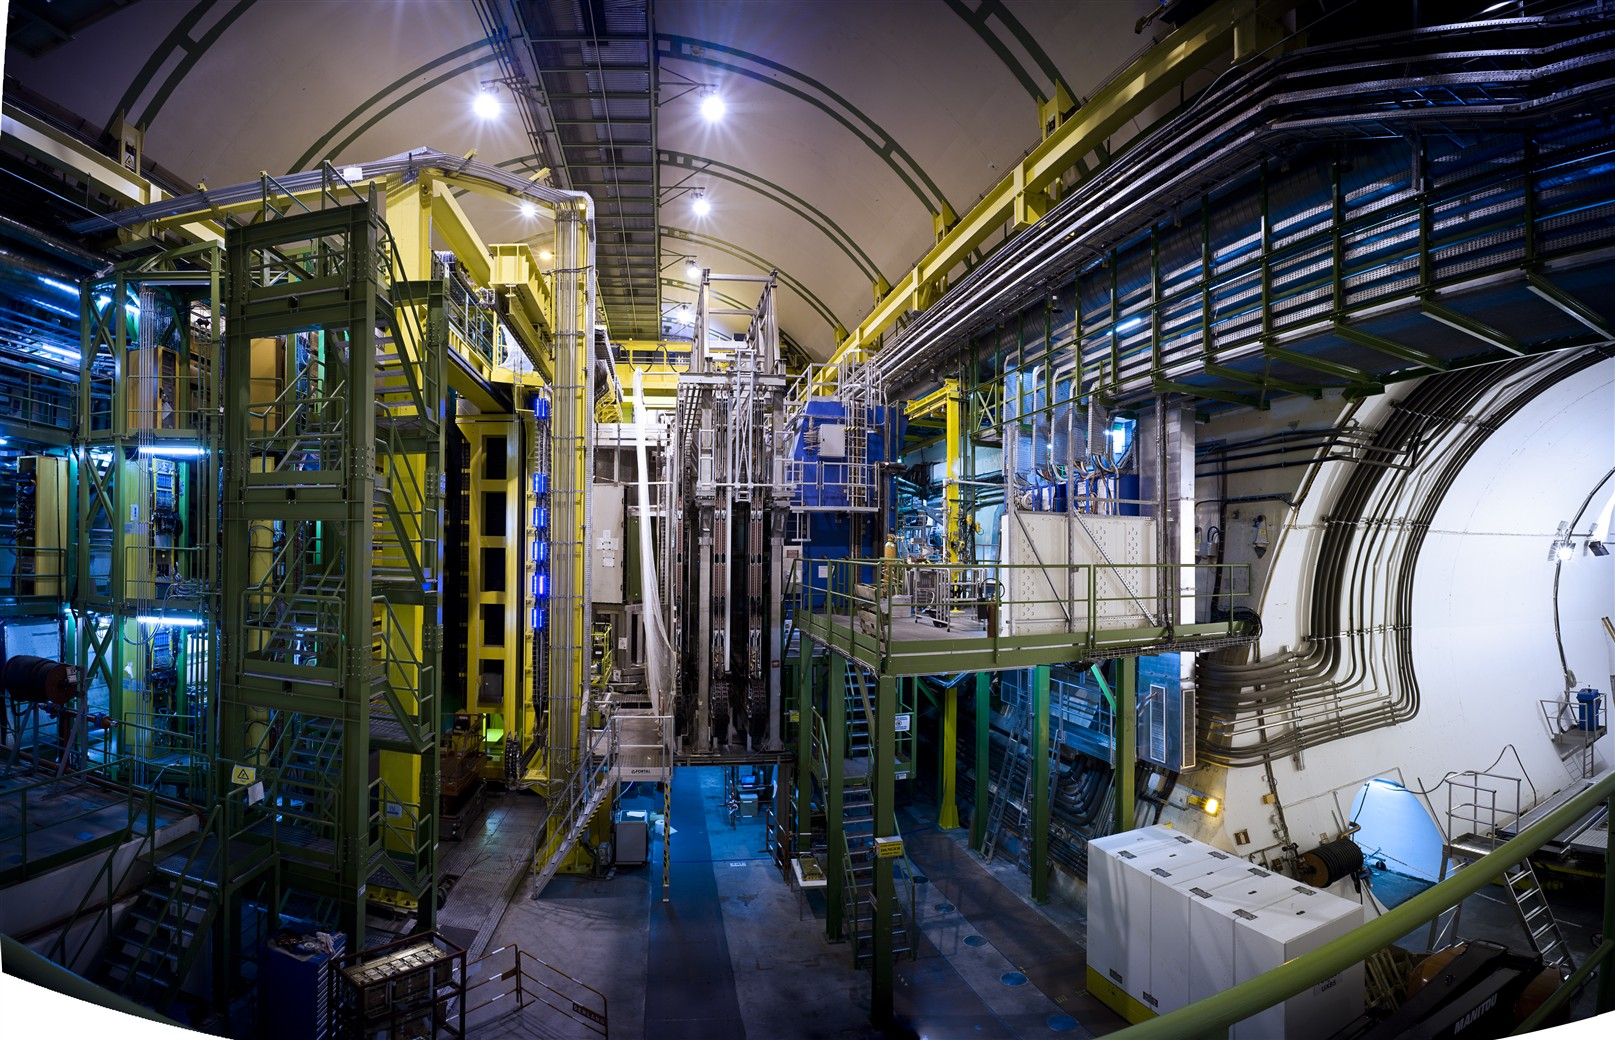
\includegraphics[width=1.05\paperwidth]{figs/cavern.jpg}}
 
 \begin{frame}[plain]
 \vspace{8.75cm}
 \hspace{-0.75cm}
 \Huge\color{anti-flashwhite}{Backup}
 \end{frame}
}

% %%%%%%%%%%%%%%%%%%%%%%%%%%%%%%%%%%%%%%%%%%%%%%%%%%%%%%%%%%%%%%%%%
% %Slide
% %%%%%%%%%%%%%%%%%%%%%%%%%%%%%%%%%%%%%%%%%%%%%%%%%%%%%%%%%%%%%%%%%
% \begin{frame}\frametitle{\bquark\bquarkbar pair production in \proton\proton collisions}

% \begin{center}
% \begin{tikzpicture}
%  \centering
%  \node[anchor=south west,inner sep=0](image) at (0,0) {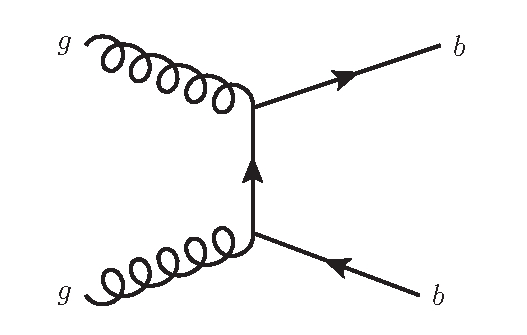
\includegraphics[width=0.4\paperwidth]{figs/detector/gluon_fusion.eps}};
%  \begin{scope}[x={(image.south east)},y={(image.north west)}]
%   %\draw[help lines,xstep=.1,ystep=.1] (0,0) grid (1,1);
%   \node[draw=none] at (0.5,-0.2) {gluon-gluon fusion};
%  \end{scope}
% \end{tikzpicture}
% \begin{tikzpicture}
%  \centering
%  \node[anchor=south west,inner sep=0](image) at (0,0) {\includegraphics[width=0.4\paperwidth]{figs/detector/quark_antiquark_annihilation.eps}};
%  \begin{scope}[x={(image.south east)},y={(image.north west)}]
%   %\draw[help lines,xstep=.1,ystep=.1] (0,0) grid (1,1);
%   \node[draw=none] at (0.5,-0.2) {quark-antiquark annihilation};
%  \end{scope}
% \end{tikzpicture}
% \end{center}

% \end{frame}

%%%%%%%%%%%%%%%%%%%%%%%%%%%%%%%%%%%%%%%%%%%%%%%%%%%%%%%%%%%%%%%%%
%Slide
%%%%%%%%%%%%%%%%%%%%%%%%%%%%%%%%%%%%%%%%%%%%%%%%%%%%%%%%%%%%%%%%%
% \begin{frame}\frametitle{}

%   \begin{center}
%   \resizebox{\columnwidth}{!}{
%     \begin{tikzpicture}
%       %\draw[step=1cm,gray,very thin] (0,0) grid (15,4);
      
%       \node[draw=none] at (2,3.5) {Beauty hadrons};
        
%       \node[draw=none,blue] at (3,1.75) {L};
%       \draw[ultra thick,dashed,blue] (2,1) -- (4,2);
%       \draw[thick] (4,2) -- (5,3.8);
%       %\node[draw=none,darkpastelgreen] at (5.3,4.05) {$\mu^{+}$};
%       \draw[thick] (4,2) -- (5.5,3.5);
%       %\node[draw=none,darkpastelgreen] at (5.75,3.75) {$\mu^{-}$};
%       \draw[thick] (4,2) -- (6,3.2);
%       \draw[thick] (4,2) -- (6.2,3.);
%       \draw[thick] (4,2) -- (6.2,2.6);
      
%       \node[draw=none] at (4.2,1.8) {SV};
        
%       \draw[ultra thick,densely dotted,darkorchid] (4,2) -- (2,0.2);
%       \draw[ultra thick,densely dotted,darkorchid] (2,1) -- (2.35,0.5);
%       \node[draw=none,darkorchid] at (2,0.5) {IP};
      
%       \node[draw=none,darkpastelred] at (2,1.6) {PV};
%       \node[draw, fill, orange, star, star points=11,scale=1.0] at (2,1){};
%       \node[draw, fill, darkpastelred, star, star points=11,scale=0.5] at (2,1){};
      
%       \draw[ultra thick,->] (0,1) -- (1.8,1);
%       \draw[ultra thick,->] (7,1) -- (2.2,1);
%       \node[draw=none] at (0.2,0.8) {\proton};
%       \node[draw=none] at (6.8,0.8) {\proton};
      
%       \node[draw=none] at (10,3.5) {Charm hadrons};
      
%       \node[draw=none,blue] at (10.5,1.5) {L};
%       \draw[ultra thick,dashed,blue] (10,1) -- (11,1.5);
%       \draw[thick] (11,1.5) -- (12.5,3.8);
%       \draw[thick] (11,1.5) -- (14,3);
        
%       \node[draw=none] at (11.3,1.35) {SV};
        
%       \draw[ultra thick,densely dotted,darkorchid] (11,1.5) -- (10,0.4);
%       \draw[ultra thick,densely dotted,darkorchid] (10,1) -- (10.3,0.7);
%       \node[draw=none,darkorchid] at (10.5,0.5) {IP};
      
%       \node[draw=none,darkpastelred] at (10,1.6) {PV};
%       \node[draw, fill, orange, star, star points=11,scale=1.0] at (10,1){};
%       \node[draw, fill, darkpastelred, star, star points=11,scale=0.5] at (10,1){};
      
%       \draw[ultra thick,->] (8,1) -- (9.8,1);
%       \draw[ultra thick,->] (15,1) -- (10.2,1);
%       \node[draw=none] at (8.2,0.8) {\proton};
%       \node[draw=none] at (14.8,0.8) {\proton};
      
%     \end{tikzpicture}
%     }
%     \bigskip
    
%     \begin{columns}
%       \begin{column}{0.49\textwidth}
%         \begin{myenv}{Beauty signatures}[linecolor=barcolor]
%           \begin{itemize}
%           \item \Bz mass 5.28 GeV
%           \begin{itemize}
%           \item[\ding{70}] daughter \pt \orderof(1 GeV)
%           \end{itemize}
%           \item $\tau \sim 1.6\ps$
%           \begin{itemize}
%           \item[\ding{70}] L $\sim 1\cm$ $\to$ large IP
%           \end{itemize}
%           %\item Common signature: displaced muon pair
%           \end{itemize}
%         \end{myenv}
%       \end{column}
%       \begin{column}{0.49\textwidth}
%         \begin{myenv}{Charm signatures}[linecolor=barcolor]
%         \begin{itemize}
%           \item \Dz mass 1.86 GeV
%           \begin{itemize}
%           \item[\ding{70}] large daughter \pt
%           \end{itemize}
%           \item $\tau \sim 0.4\ps$
%           \begin{itemize}
%           \item[\ding{70}] L $\sim 0.4 \cm$ $\to$ smaller IP
%           \end{itemize}
%           %\item Common signature: displaced muon pair
%           \end{itemize}
%         \end{myenv}
%       \end{column}
%     \end{columns}
    
%   \end{center}
% \end{frame}

% %%%%%%%%%%%%%%%%%%%%%%%%%%%%%%%%%%%%%%%%%%%%%%%%%%%%%%%%%%%%%%%%%
% %Slide
% %%%%%%%%%%%%%%%%%%%%%%%%%%%%%%%%%%%%%%%%%%%%%%%%%%%%%%%%%%%%%%%%%
\begin{frame}\frametitle{Tracking definitions}

\begin{equation*}
\text{Reconstruction efficiency} = \frac{N_{\text{reconstructible~and~reconstructed}}}{N_{\text{reconstructible}}}
\end{equation*}

\bigskip

\begin{columns}
\begin{column}{0.2\textwidth}
\end{column}
\begin{column}{0.6\textwidth}
\begin{myenv}{Reconstructible requirements}[linecolor=barcolor]
\centering
  \begin{tabular}{c|c}
    Common req. & Upstream req.\\
    \hline
    !electron & Reco. in VELO\\
    $2<\eta<5$ & 3+ TT layers fired\\
    $\pt>0.5\gevc$ \\
    \bquark-hadron daughter \\
    \velo + T hits \\
  \end{tabular}
\end{myenv}
\end{column}
\begin{column}{0.2\textwidth}
\end{column}
\end{columns}
\end{frame}

% %%%%%%%%%%%%%%%%%%%%%%%%%%%%%%%%%%%%%%%%%%%%%%%%%%%%%%%%%%%%%%%%%
% %Slide
% %%%%%%%%%%%%%%%%%%%%%%%%%%%%%%%%%%%%%%%%%%%%%%%%%%%%%%%%%%%%%%%%%
\begin{frame}\frametitle{Tracking definitions}

\begin{equation*}
\text{Ghost rate}  = \frac{N_{\text{ghost~tracks}}}{N_{\text{tracks}}}
\end{equation*}

\bigskip

\begin{columns}
\begin{column}{0.25\textwidth}
\end{column}
\begin{column}{0.5\textwidth}
\begin{myenv}{Track requirements}[linecolor=barcolor]
\centering
\begin{tabular}{c}
  $2<\eta<5$ \\
  $\pt>0.5\gevc$ \\
\end{tabular}
\medskip
\end{myenv}
\end{column}
\begin{column}{0.25\textwidth}
\end{column}
\end{columns}
\end{frame}

% %%%%%%%%%%%%%%%%%%%%%%%%%%%%%%%%%%%%%%%%%%%%%%%%%%%%%%%%%%%%%%%%%
% %Slide
% %%%%%%%%%%%%%%%%%%%%%%%%%%%%%%%%%%%%%%%%%%%%%%%%%%%%%%%%%%%%%%%%%
\begin{frame}\frametitle{VeloUT: Wrong side tracks}

\begin{itemize}
  \item Fraction of truth matched tracks with at least one hit on the opposite side of the extrapolated \velo track in the $x$-$z$ plane
\end{itemize}

\begin{center}
\includegraphics[width=0.4\textwidth]{figs/upstream-tracking-upgrade/wrong_side_hits.pdf}
\end{center}
\end{frame}

%%%%%%%%%%%%%%%%%%%%%%%%%%%%%%%%%%%%%%%%%%%%%%%%%%%%%%%%%%%%%%%%
%% Slide
%%%%%%%%%%%%%%%%%%%%%%%%%%%%%%%%%%%%%%%%%%%%%%%%%%%%%%%%%%%%%%%%
\begin{frame}{Upstream tracking for \lhcb Run 2 (2015-2018)}

\begin{itemize}
  \item[$\blacktriangleright$] Following improved performance achieved using upstream tracks, similar strategy developed for Run 2
  \item[$\blacktriangleright$]   New VeloTT algorithm created based on the optimised VeloUT algorithm
  \begin{itemize}
    \item[\ding{80}] Similar improvements achieved
    \item[\ding{80}] Allows IP requirements to be removed
    \item[\ding{80}] Adopted into the default tracking sequence for the first stage of the HLT
  \end{itemize}
\end{itemize}

\begin{itemize}
  \item[\ding{80}] Greatly improved signal efficiency for charm physics
  \item[\ding{80}] Lifetime unbiased triggering on hadronic final states for first time
\end{itemize}

\begin{itemize}
\item[\ding{80}] First HEP experiment to implement fully automatic tracking system alignment, PID calibration and track reconstruction online
\end{itemize}

\end{frame}

%%%%%%%%%%%%%%%%%%%%%%%%%%%%%%%%%%%%%%%%%%%%%%%%%%%%%%%%%%%%%%%%%
%Slide
%%%%%%%%%%%%%%%%%%%%%%%%%%%%%%%%%%%%%%%%%%%%%%%%%%%%%%%%%%%%%%%%%
\begin{frame}{VeloTT: Optimised peformance}

\begin{columns}
\begin{column}{0.65\textwidth}
\begin{itemize}
  \item Large improvement in the efficiency ($+5$\%)
  \begin{itemize}
    \item[\ding{70}] Now flat in \ptot
  \end{itemize}
  \item Huge reduction in the execution time ($\times$65!)
  \item Slight increase in the ghost rate ($+4$\%)
  \begin{itemize}
    \item[\ding{70}] Can be reduced in offline analysis
  \end{itemize}
\end{itemize}

\bigskip

\begin{mdframed}[linecolor=barcolor]
\begin{center}
\resizebox{\columnwidth}{!}{
\begin{tabular}{c|c|c|c}
  \velott & Efficiency [\%] & Ghost rate [\%] & Timing [ms] \\ 
  \hline
  Run I  &  92.74  &  7.21  &  32.50  \\
  Run II  &  97.77  &  11.60  &  \hphantom{0}0.50   \\
 \end{tabular}
 }
\end{center}
\end{mdframed}
\end{column}

\begin{column}{0.35\textwidth}
\centering
\begin{figure}
\vspace*{-1cm}
\includegraphics[height=0.475\textheight]{figs/upstream-tracking-run2/VeloTT-eff-p.pdf}\\
\includegraphics[height=0.475\textheight]{figs/upstream-tracking-run2/VeloTT-gr-p.pdf}
\end{figure}
\end{column}
\end{columns}

\end{frame}

%%%%%%%%%%%%%%%%%%%%%%%%%%%%%%%%%%%%%%%%%%%%%%%%%%%%%%%%%%%%%%%%%
%Slide
%%%%%%%%%%%%%%%%%%%%%%%%%%%%%%%%%%%%%%%%%%%%%%%%%%%%%%%%%%%%%%%%%
\begin{frame}{VeloTT-Forward: Optimised peformance}

\begin{columns}
\begin{column}{0.65\textwidth}
\begin{itemize}
  \item Significant reduction in the execution time ($\times$3)
  \item Large reduction in the ghost rate ($\times$3)
  \item Some loss of efficiency ($-4$\%)
\end{itemize}

\bigskip

\begin{mdframed}[linecolor=barcolor]
\begin{center}
\resizebox{\columnwidth}{!}{
\begin{tabular}{c|c|c|c}
    & Efficiency [\%] & Ghost rate [\%] & Timing [ms] \\
   \hline
  Velo-Forward  & 93.15  & 46.86  &  13.71 \\
  VeloTT-Forward  & 89.23  & 17.13  &  0.50+4.08 \\
 \end{tabular}
 }
\end{center}
\end{mdframed}
\end{column}

\begin{column}{0.35\textwidth}
\centering
\begin{figure}
\vspace*{-1cm}
\includegraphics[height=0.475\textheight]{figs/upstream-tracking-run2/Forward-eff-p.pdf}\\
\includegraphics[height=0.475\textheight]{figs/upstream-tracking-run2/Forward-gr-p.pdf}
\end{figure}
\end{column}
\end{columns}

\end{frame}

%%%%%%%%%%%%%%%%%%%%%%%%%%%%%%%%%%%%%%%%%%%%%%%%%%%%%%%%%%%%%%%%%
%Slide
%%%%%%%%%%%%%%%%%%%%%%%%%%%%%%%%%%%%%%%%%%%%%%%%%%%%%%%%%%%%%%%%%
\begin{frame}{Theoretical formalism}

\begin{itemize}
  \item Rare \bquark-hadron decays are a multi-scale problem: $m_{W} \gg m_{\bquark} > \Lambda_{\rm QCD}$
  \item Measurements interpreted in Operator Product Expansion framework
  \begin{itemize}
  \item[\ding{70}] All degrees of freedom above a given energy scale are integrated out
  \item[\ding{70}] Introduce set of Wilson coefficients, $\mathcal{C}_{i}$, and local operators, $\mathcal{O}_{i}$, encoding coupling strength and Lorentz structure
  \end{itemize}
\end{itemize}
\begin{equation*}
\mathcal{H}_{\rm eff} = - \frac{4G_{F}}{\sqrt{2}}V_{tb}V^{*}_{ts}\sum_{i}(\mathcal{C}_{i}^{\rm SM}+\mathcal{C}_{i}^{\rm NP})\mathcal{O}_{i}
\end{equation*}
  
\begin{itemize}
\item \btosmm transitions sensitive to $\mathcal{C}_{7}$, $\mathcal{C}_{9}$, $\mathcal{C}_{10}$
\end{itemize}

\medskip

\centering
\begin{tikzpicture}
\node[anchor=south west,inner sep=0](image) at (0,0) {\includegraphics[width=0.3\textwidth]{figs/theory/btosll_penguin.eps}};
\begin{scope}[x={(image.south east)},y={(image.north west)}]
%\draw[help lines,xstep=.1,ystep=.1] (0,0) grid (1,1);
\node[draw=none] at (0.53,0.96) {\scriptsize \Wm};
\node[draw=none] at (0.3,0.6) {\scriptsize \tquark};
\node[draw=none] at (0.56,0.27) {\scriptsize {\small\color{bleudefrance}{\Pgamma}}\color{black}{,} \color{bostonuniversityred}{$\Z^{0}$}};
\end{scope}
\end{tikzpicture}
\begin{tikzpicture}
\node[anchor=south west,inner sep=0](image) at (0,0) {\includegraphics[width=0.3\textwidth]{figs/theory/btosll_effective.eps}};
\begin{scope}[x={(image.south east)},y={(image.north west)}]
%\draw[help lines,xstep=.1,ystep=.1] (0,0) grid (1,1);
\node[draw=none] at (0.53,0.58) {\scriptsize \color{bleudefrance}{$\mathcal{C}_{7}$}\color{black}{,} \color{bostonuniversityred}{$\mathcal{C}_{9,10}$}};
\end{scope}
\end{tikzpicture}
\end{frame}

%%%%%%%%%%%%%%%%%%%%%%%%%%%%%%%%%%%%%%%%%%%%%%%%%%%%%%%%%%%%%%%%%
%Slide
%%%%%%%%%%%%%%%%%%%%%%%%%%%%%%%%%%%%%%%%%%%%%%%%%%%%%%%%%%%%%%%%%
\begin{frame}{Operators}

\begin{alignat*}{2}
&\order_{7} = \frac{e}{g^{2}}m_{\bquark}(\squarkbar\sigma_{\mu\nu}P_{R}\bquark)F^{\mu\nu}~~~~~~~&&\order_{7}^{\prime} = \frac{e}{g^{2}}m_{\bquark}(\squarkbar\sigma_{\mu\nu}P_{L}\bquark)F^{\mu\nu} \nonumber \\
&\order_{9} = \frac{e^{2}}{g^{2}}(\squarkbar\gamma_{\mu}P_{L}\bquark)(\ellbar\gamma^{\mu}\ell) &&\order_{9}^{\prime} = \frac{e^{2}}{g^{2}}(\squarkbar\gamma_{\mu}P_{R}\bquark)(\ellbar\gamma^{\mu}\ell) \nonumber \\
&\order_{10} = \frac{e^{2}}{g^{2}}(\squarkbar\gamma_{\mu}P_{L}\bquark)(\ellbar\gamma^{\mu}\gamma_{5}\ell) &&\order_{10}^{\prime} = \frac{e^{2}}{g^{2}}(\squarkbar\gamma_{\mu}P_{R}\bquark)(\ellbar\gamma^{\mu}\gamma_{5}\ell) \\
&\order_{S} = \frac{e^{2}}{16\pi^{2}}m_{\bquark}(\squarkbar P_{R}\bquark)(\ellbar\ell) &&\order_{S}^{\prime} = \frac{e^{2}}{16\pi^{2}}m_{\bquark}(\squarkbar P_{L}\bquark)(\ellbar\ell) \nonumber\\
&\order_{P} = \frac{e^{2}}{16\pi^{2}}m_{\bquark}(\squarkbar P_{R}\bquark)(\ellbar\gamma_{5}\ell) &&\order_{P}^{\prime} = \frac{e^{2}}{16\pi^{2}}m_{\bquark}(\squarkbar P_{L}\bquark)(\ellbar\gamma_{5}\ell) \nonumber
\end{alignat*}

\end{frame}

%%%%%%%%%%%%%%%%%%%%%%%%%%%%%%%%%%%%%%%%%%%%%%%%%%%%%%%%%%%%%%%%%
%Slide
%%%%%%%%%%%%%%%%%%%%%%%%%%%%%%%%%%%%%%%%%%%%%%%%%%%%%%%%%%%%%%%%%
\begin{frame}{Interpretation}
\begin{columns}
\begin{column}{0.5\textwidth}

\begin{tikzpicture}
 \centering
 \node[anchor=south west,inner sep=0](image) at (0,0) {\includegraphics[trim={2.5cm 20cm 10.7cm 2.4cm},clip,width=1.0\textwidth]{figs/kpimm/introduction/c9c10.pdf}};
 \begin{scope}[x={(image.south east)},y={(image.north west)}]
 %\draw[help lines,xstep=.1,ystep=.1] (0,0) grid (1,1);
  \node[draw=none] at (0.32,0.94) {\bf \scriptsize [arXiv:1503.06199]};
\end{scope}
\end{tikzpicture}
\centering

{\color{applegreen}{Branching fractions}}, {\color{antiquebrass}{angular observables}}, {\color{airforceblue}{combined}} 
\end{column}
\begin{column}{0.5\textwidth}
\begin{itemize}
\item Several attempts to interpret LHCb data by performing global fits
\item Consistent picture, data favours modified vector coupling ($\mathcal{C}_{9}^{\rm NP}$) at $\sim[3,4]\sigma$
\end{itemize}

\bigskip

\begin{myenv}{Possible interpretation}[linecolor=barcolor]
\begin{itemize}
\setlength{\itemindent}{0.5em}
\item NP physics scenario, e.g. new vector $Z^{'}$, leptoquarks, etc
\item Problem with our understanding of QCD, e.g. not properly estimating contribution from charm loops
\end{itemize}
\end{myenv}

\end{column}
\end{columns}
\end{frame}

%%%%%%%%%%%%%%%%%%%%%%%%%%%%%%%%%%%%%%%%%%%%%%%%%%%%%%%%%%%%%%%%%
%Slide
%%%%%%%%%%%%%%%%%%%%%%%%%%%%%%%%%%%%%%%%%%%%%%%%%%%%%%%%%%%%%%%%%
\begin{frame}{\BdToKpimm in the \Kstarfourteenthirty region \hspace{0pt plus 1 filll} {\small \bf \textcolor{black}{[JHEP 12 (2016) 065]}}}
\begin{itemize}
\item[$\blacktriangleright$] Measurements performed in $1330<\mkpi<1530\mevcc$ region at low \qsq
\item[]
\item[\ding{182}] Differential branching fraction as a function of \qsq
  \begin{itemize}
    \item[\ding{70}] 5 \qsq bins: [0.1,\,0.98], [1.1,\,2.5], [2.5,\,4.0], [4.0,\,6.0], [6.0,\,8.0]~\gevgevcccc
    \item[\ding{70}] Normalised to \BdToJPsiKstP
    \item[\ding{70}] Never previously measured
  \end{itemize}
\item[\ding{183}] Angular analysis
  \begin{itemize}
    \item[\ding{70}] Single \qsq bin: [1.1,\,6.0]~\gevgevcccc
    \item[\ding{70}] S-, P- and D-wave contributions considered for first time
    \item[\ding{70}] Requires new orthonormal basis of angular functions 
    % \item[\ding{70}] 40 normalised moments ($\overline{\Gamma}_{2}$-$\overline{\Gamma}_{41}$)
  \end{itemize}
  
\end{itemize}
\end{frame}

%%%%%%%%%%%%%%%%%%%%%%%%%%%%%%%%%%%%%%%%%%%%%%%%%%%%%%%%%%%%%%%%%
%Slide
%%%%%%%%%%%%%%%%%%%%%%%%%%%%%%%%%%%%%%%%%%%%%%%%%%%%%%%%%%%%%%%%%
\begin{frame}{Selection of \BdToKpimm signal candidates}

\vspace{-0.5cm}

\begin{itemize}
 \item[\ding{80}] Analysis performed using the full \lhcb Run I data sample (3\invfb)
\end{itemize}

\begin{itemize}
  \item[$\blacktriangleright$] Candidates are required to have `fired' trigger at each stage
  \item[$\blacktriangleright$] Cut based selection applied to select candidates of the form $\decay{\Bz}{X\mumu}$
  \item[$\blacktriangleright$] Multivariate classifier used to reduce combinatorial background
  \begin{itemize}
  \item[\ding{70}] Kinematic, isolation and PID variables used as input
  \end{itemize}
  \item[$\blacktriangleright$] Exclusive backgrounds removed by specific vetoes
  \begin{itemize}
  \item[\ding{70}] \BdToKpimm ($\kaon \leftrightarrow \pion$) 
  \item[\ding{70}] \BdToJPsiKpi ($\pion \leftrightarrow \muon$, $\kaon \leftrightarrow \muon$) 
  \item[\ding{70}] \BdToPsitwosKpi ($\pion \leftrightarrow \muon$, $\kaon \leftrightarrow \muon$) 
  \item[\ding{70}] \LbTopKmm ($\proton \to \pion$, $\proton \to \kaon~\&~\kaon \to \pion$) 
  \item[\ding{70}] \BuToKmm (random \pion) 
  \end{itemize}
\end{itemize}

\tikzoverlay at (9cm,3cm) {
\begin{tikzpicture}
\node[anchor=south west,inner sep=0](image) at (0,0) {\includegraphics[width=4.5cm]{figs/kpimm/selection/jpsi_pimu_fit.pdf}};
\node[draw=none] at (1.15,4.5) {\tiny $\BdToJPsiKpi mis$-$id$};
\end{tikzpicture} 
};

\end{frame}

%%%%%%%%%%%%%%%%%%%%%%%%%%%%%%%%%%%%%%%%%%%%%%%%%%%%%%%%%%%%%%%%%
%Slide
%%%%%%%%%%%%%%%%%%%%%%%%%%%%%%%%%%%%%%%%%%%%%%%%%%%%%%%%%%%%%%%%%
\begin{frame}{\BdToKpimm: Expected resonant contributions}

\begin{center}
\begin{tabular}{c|c|c|c|r}
Resonance & ${\rm J}^{P}$ & Mass [$\mathrm{Me\kern -0.1em V\!/}c^2$] & Full width [$\mathrm{Me\kern -0.1em V\!/}c^2$]  & $\mathcal{B}(K\pi)~[\%]$ \\
\hline
$K^\ast(1410)^0$ & $1^{-}$& $\hphantom{0.}1414 \pm 15\hphantom{.}$& $232 \pm 21\hphantom{0}$  & $6.6 \pm 1.3$ \\
$K^\ast_0(1430)^0$ & $0^{+}$ & $\hphantom{0.}1425 \pm 50\hphantom{.}$ & $270 \pm 80\hphantom{0}$ & $\hphantom{.}93 \pm 10\hphantom{.}$ \\
$K^\ast_2(1430)^0$ & $2^{+}$ & $1432.4\pm 1.3$ & $109 \pm 5\hphantom{00}$ & $49.9 \pm 1.2$ \\
$K^\ast(1680)^0$ & $1^{-}$ & $\hphantom{0.}1717 \pm 27\hphantom{.}$ & $322 \pm 110$ & $38.7 \pm 2.5$ \\
$K^\ast_3(1780)^0$ & $3^{-}$ & $\hphantom{0.}1776 \pm 7\hphantom{0.}$ & $159 \pm 21\hphantom{0}$ & $18.8 \pm 1.0$ \\
$K^\ast_4(2045)^0$ & $4^{+}$ & $\hphantom{0.}2045 \pm 9\hphantom{0.}$ & $198 \pm 30\hphantom{0}$ & $9.9 \pm 1.2$ \\
\end{tabular}
\end{center}

\end{frame}

%%%%%%%%%%%%%%%%%%%%%%%%%%%%%%%%%%%%%%%%%%%%%%%%%%%%%%%%%%%%%%%%%
%Slide
%%%%%%%%%%%%%%%%%%%%%%%%%%%%%%%%%%%%%%%%%%%%%%%%%%%%%%%%%%%%%%%%%
\begin{frame}{\BdToKpimm: Angular moments analysis}
 
\begin{itemize}
\item The transversity-basis moments of the first 10 (of 41) orthonormal angular functions
 
 \medskip
 
 \resizebox{0.9\textwidth}{!}{
   \begin{tabular}{c|c|c|c}
     $i$    &   $f_i(\Omega)$             & $\mathrm{\Gamma}^{L, {\rm tr}}_i(\qsq)$ & $\eta^{L\to R}_i$  \\ \hline \hline
     1   &   $P^0_0 Y^0_0$     &  $\left[ \hzsq + \hpasq + \hpesq + \ssq + \dzsq + \dpasq + \dpesq\right]$ & + ($L \to R$)\\ \hline
     2   &   $P^0_1 Y^0_0$     &  $2\left[\frac{2}{\sqrt{5}} \rhzdz + \rshz + \sqrt{\frac{3}{5}}  \rel( H^L_\parallel D^{L\ast}_\parallel + H^L_\perp D^{L\ast}_\perp  )\right]$ & " \\ \hline
     3   &   $P^0_2 Y^0_0$     &  $\frac{\sqrt{5}}{7}$ (\dpasq + \dpesq) - $\frac{1}{\sqrt{5}}$ (\hpasq + \hpesq) + $\frac{2}{\sqrt{5}}$ \hzsq  + $\frac{10}{7\sqrt{5}}$ \dzsq + $2$ \rsdz & " \\  \hline
     4   &   $P^0_3 Y^0_0$     &  $\frac{6}{\sqrt{35}} \left[ - \rel(H^L_\parallel D^{L\ast}_\parallel +  H^L_\perp D^{L\ast}_\perp)  + \sqrt{3} \rhzdz  \right]$ & "\\  \hline
     5   &   $P^0_4 Y^0_0$     &  $\frac{2}{7} \left[ -2 (\dpasq + \dpesq) + 3 \dzsq \right] $ & "\\  \hline
     6   &   $P^0_0 Y^0_2$     &  $\frac{1}{2 \sqrt{5}} \left[ (\dpasq + \dpesq) + (\hpasq + \hpesq) - 2 \ssq - 2 \dzsq - 2 \hzsq \right]$ & " \\  \hline
     7   &   $P^0_1 Y^0_2$     &  $\left[ \frac{\sqrt{3}}{5} \rel(H^L_\parallel D^{L\ast}_\parallel  + H^L_\perp D^{L\ast}_\perp) - \frac{2}{\sqrt{5}} \rel(S^L H^{L\ast}_0)  - \frac{4}{5} \rel(H^L_0 D^{L\ast}_0)\right] $ & "  \\ \hline
     8   &   $P^0_2 Y^0_2$     &  $ \left[ \frac{1}{14} (\dpasq + \dpesq) - \frac{2}{7} \dzsq - \frac{1}{10} (\hpasq + \hpesq) - \frac{2}{5} \hzsq - \frac{2}{\sqrt{5}} \rsdz \right]$ & "  \\  \hline
     9   &   $P^0_3 Y^0_2$     &  $ - \frac{3}{5 \sqrt{7}} \left[ \rel( H^L_\parallel D^{L \ast}_\parallel + H^L_\perp D^{L \ast}_\perp) + 2 \sqrt{3} \rel(H^L_0 D^{L \ast}_0 ) \right] $ & "\\  \hline
     10  &   $P^0_4 Y^0_2$     &  $ -\frac{2}{7 \sqrt{5}}  \left[ \dpasq + \dpesq + 3 \dzsq \right] $ & "  \\
   \end{tabular}
 }
 
\medskip
 
\item The S-, P- and D-wave transversity amplitudes are denoted as $S^{\{L,R\}}$, $H^{\{L,R\}}_{\{0,\parallel,\perp\}}$ and $D^{\{L,R\}}_{\{0,\parallel,\perp\}}$, respectively.
\end{itemize}
\end{frame}

%%%%%%%%%%%%%%%%%%%%%%%%%%%%%%%%%%%%%%%%%%%%%%%%%%%%%%%%%%%%%%%%
%Slide
%%%%%%%%%%%%%%%%%%%%%%%%%%%%%%%%%%%%%%%%%%%%%%%%%%%%%%%%%%%%%%%%%
\begin{frame}{\BdToKpimm: Angular moments analysis}
\begin{itemize}
  \item Distributions of the decays angles within $\pm$50\mevcc of the nominal \Bz mass
  \begin{itemize}
    \item Blue: estimated signal distribution obtained from the angular moments model
    \item Red: projected background from upper mass sideband
  \end{itemize}
\end{itemize}

\medskip

\centering
\includegraphics[width=0.32\textwidth]{figs/kpimm/angular-analysis/costhetal.pdf}
\includegraphics[width=0.32\textwidth]{figs/kpimm/angular-analysis/costhetak.pdf}
\includegraphics[width=0.32\textwidth]{figs/kpimm/angular-analysis/phi.pdf}
\end{frame}

%%%%%%%%%%%%%%%%%%%%%%%%%%%%%%%%%%%%%%%%%%%%%%%%%%%%%%%%%%%%%%%%%
%Slide
%%%%%%%%%%%%%%%%%%%%%%%%%%%%%%%%%%%%%%%%%%%%%%%%%%%%%%%%%%%%%%%%%
\begin{frame}{\BdToKpimm: Systematic uncertainties}

\begin{itemize}
  \item Systematics uncertainties are small ($<30\%$ of statistical uncertainty)
  \item Dominant systematic uncertainty on $\deriv\BF/\deriv\qsq$ due to uncertainty on \mbox{\BF(\BdToJPsiKstP)}
\end{itemize}

\bigskip

\begin{mdframed}[linecolor=barcolor]
\begin{center}
\begin{tabular}{l|cc}
\multicolumn{1}{c|}{Source} & $d\BF/d\qsq \times 10^{-8}~[c^{4}/\gev^{2}]$ & $\overline{\Gamma}_{i}$ \\
\hline
Acceptance stat.\! uncertainty & 0.006--0.030 & 0.003--0.013 \\
Data-simulation differences & 0.001--0.014 & 0.001--0.007 \\
Peaking backgrounds & 0.013--0.026 & 0.001--0.040 \\
\hline
$\BF(\BdToJPsiKstP)$ & 0.033--0.110 & -- \\
\end{tabular}
\end{center}
\end{mdframed}
\end{frame}

%%%%%%%%%%%%%%%%%%%%%%%%%%%%%%%%%%%%%%%%%%%%%%%%%%%%%%%%%%%%%%%%%
%Slide
%%%%%%%%%%%%%%%%%%%%%%%%%%%%%%%%%%%%%%%%%%%%%%%%%%%%%%%%%%%%%%%%%
\begin{frame}{\BdToKpimm: Differential branching fraction}
\begin{center}
\begin{tabular}{lc}
\qsq [$\gevgevcccc$] & $\deriv\BF/\deriv\qsq \times 10^{-8}~[c^{4}/\gev^{2}]$ \\
\hline
$[0.10,0.98]$ & 1.60 $\pm$ 0.28 $\pm$ 0.04 $\pm$ 0.11 \\
$[1.10,2.50]$ & 1.14 $\pm$ 0.19 $\pm$ 0.03 $\pm$ 0.08 \\
$[2.50,4.00]$ & 0.91 $\pm$ 0.16 $\pm$ 0.03 $\pm$ 0.06 \\
$[4.00,6.00]$ & 0.56 $\pm$ 0.12 $\pm$ 0.02 $\pm$ 0.04 \\
$[6.00,8.00]$ & 0.49 $\pm$ 0.11 $\pm$ 0.01 $\pm$ 0.03 \\
\hline
$[1.10,6.00]$ & 0.82 $\pm$ 0.09 $\pm$ 0.02 $\pm$ 0.06 \\
\end{tabular}
\end{center}
\end{frame}

%%%%%%%%%%%%%%%%%%%%%%%%%%%%%%%%%%%%%%%%%%%%%%%%%%%%%%%%%%%%%%%%%
%Slide
%%%%%%%%%%%%%%%%%%%%%%%%%%%%%%%%%%%%%%%%%%%%%%%%%%%%%%%%%%%%%%%%%
\begin{frame}{Angular moments analysis}

\begin{itemize}
\item Normalised moments for $i \in \{2,...,41\}$ defined as
\end{itemize}
\begin{equation*}
\overline{\Gamma}_i(\qsq) = \frac{\Gamma_{i}(\qsq)}{\Gamma_{1}(\qsq)}
\end{equation*}
\begin{itemize}
\item Covariance matrix for $i,j \in \{2,...,41\}$ computed as
\end{itemize}

\begin{equation*}
\overline{C}_{ij} = \left[C_{ij} + \frac{\Gamma_i \Gamma_j}{\Gamma_1^2} C_{11} - \frac{\Gamma_i C_{1j} + \Gamma_j C_{1i}}{\Gamma_1}\right] \frac{1}{\Gamma_1^2}
\end{equation*}

\begin{itemize}
\item[\ding{80}] Can also estimate D-wave fraction
\end{itemize}

\begin{equation*}
F_{\rm D} \equiv  \displaystyle - \frac{7}{18} \left(2\,\overline{\Gamma}_{5} + 5 \sqrt{5}\,\overline{\Gamma}_{10} \right)
\end{equation*}

\end{frame}

%%%%%%%%%%%%%%%%%%%%%%%%%%%%%%%%%%%%%%%%%%%%%%%%%%%%%%%%%%%%%%%%%
%Slide
%%%%%%%%%%%%%%%%%%%%%%%%%%%%%%%%%%%%%%%%%%%%%%%%%%%%%%%%%%%%%%%%%
\begin{frame}{\BdToKpimm: Angular moments analysis}
\begin{columns}
\begin{column}{0.2\textwidth}
\end{column}
\begin{column}{0.6\textwidth}
\centering
\vspace{-1cm}
\resizebox{0.85\textheight}{!}{%
\begin{tabular}{l|c}
$\overline{\Gamma}_{i}$ & Value \\ 
\hline
$\overline{\Gamma}_{2}$ & $-0.42$ $\pm$ 0.13 $\pm$ 0.03 \\ 
$\overline{\Gamma}_{3}$ & $-0.38$ $\pm$ 0.15 $\pm$ 0.01 \\ 
$\overline{\Gamma}_{4}$ & $-0.02$ $\pm$ 0.14 $\pm$ 0.01 \\ 
$\overline{\Gamma}_{5}$ & \hphantom{$-$}0.29 $\pm$ 0.14 $\pm$ 0.02 \\ 
$\overline{\Gamma}_{6}$ & $-0.05$ $\pm$ 0.14 $\pm$ 0.04 \\ 
$\overline{\Gamma}_{7}$ & $-0.06$ $\pm$ 0.15 $\pm$ 0.03 \\ 
$\overline{\Gamma}_{8}$ & \hphantom{$-$}0.04 $\pm$ 0.16 $\pm$ 0.01 \\ 
$\overline{\Gamma}_{9}$ & \hphantom{$-$}0.05 $\pm$ 0.16 $\pm$ 0.02 \\ 
$\overline{\Gamma}_{10}$ & \hphantom{$-$}0.24 $\pm$ 0.17 $\pm$ 0.02 \\ 
$\overline{\Gamma}_{11}$ & \hphantom{$-$}0.06 $\pm$ 0.13 $\pm$ 0.01 \\ 
$\overline{\Gamma}_{12}$ & $-0.01$ $\pm$ 0.13 $\pm$ 0.02 \\ 
$\overline{\Gamma}_{13}$ & $-0.08$ $\pm$ 0.12 $\pm$ 0.01 \\ 
$\overline{\Gamma}_{14}$ & \hphantom{$-$}0.09 $\pm$ 0.13 $\pm$ 0.01 \\ 
$\overline{\Gamma}_{15}$ & \hphantom{$-$}0.11 $\pm$ 0.13 $\pm$ 0.00 \\ 
$\overline{\Gamma}_{16}$ & $-0.12$ $\pm$ 0.13 $\pm$ 0.01 \\ 
$\overline{\Gamma}_{17}$ & $-0.04$ $\pm$ 0.13 $\pm$ 0.01 \\ 
$\overline{\Gamma}_{18}$ & \hphantom{$-$}0.03 $\pm$ 0.14 $\pm$ 0.01 \\ 
$\overline{\Gamma}_{19}$ & \hphantom{$-$}0.11 $\pm$ 0.11 $\pm$ 0.01 \\ 
$\overline{\Gamma}_{20}$ & $-0.00$ $\pm$ 0.11 $\pm$ 0.01 \\ 
$\overline{\Gamma}_{21}$ & \hphantom{$-$}0.03 $\pm$ 0.12 $\pm$ 0.01 \\ 
\end{tabular}
\hspace{1em}
\begin{tabular}{l|c}
$\overline{\Gamma}_{i}$ & Value \\ 
\hline
$\overline{\Gamma}_{22}$ & \hphantom{$-$}0.21 $\pm$ 0.12 $\pm$ 0.01 \\ 
$\overline{\Gamma}_{23}$ & \hphantom{$-$}0.03 $\pm$ 0.12 $\pm$ 0.01 \\ 
$\overline{\Gamma}_{24}$ & $-0.10$ $\pm$ 0.10 $\pm$ 0.01 \\ 
$\overline{\Gamma}_{25}$ & \hphantom{$-$}0.03 $\pm$ 0.10 $\pm$ 0.01 \\ 
$\overline{\Gamma}_{26}$ & \hphantom{$-$}0.08 $\pm$ 0.11 $\pm$ 0.01 \\ 
$\overline{\Gamma}_{27}$ & \hphantom{$-$}0.14 $\pm$ 0.11 $\pm$ 0.01 \\ 
$\overline{\Gamma}_{28}$ & $-0.04$ $\pm$ 0.11 $\pm$ 0.01 \\ 
$\overline{\Gamma}_{29}$ & \hphantom{$-$}0.06 $\pm$ 0.15 $\pm$ 0.04 \\ 
$\overline{\Gamma}_{30}$ & $-0.21$ $\pm$ 0.15 $\pm$ 0.04 \\ 
$\overline{\Gamma}_{31}$ & $-0.07$ $\pm$ 0.16 $\pm$ 0.01 \\ 
$\overline{\Gamma}_{32}$ & $-0.16$ $\pm$ 0.17 $\pm$ 0.02 \\ 
$\overline{\Gamma}_{33}$ & $-0.04$ $\pm$ 0.17 $\pm$ 0.02 \\ 
$\overline{\Gamma}_{34}$ & \hphantom{$-$}0.15 $\pm$ 0.11 $\pm$ 0.01 \\ 
$\overline{\Gamma}_{35}$ & $-0.13$ $\pm$ 0.11 $\pm$ 0.01 \\ 
$\overline{\Gamma}_{36}$ & \hphantom{$-$}0.05 $\pm$ 0.11 $\pm$ 0.01 \\ 
$\overline{\Gamma}_{37}$ & \hphantom{$-$}0.05 $\pm$ 0.11 $\pm$ 0.01 \\ 
$\overline{\Gamma}_{38}$ & \hphantom{$-$}0.06 $\pm$ 0.11 $\pm$ 0.00 \\ 
$\overline{\Gamma}_{39}$ & $-0.08$ $\pm$ 0.11 $\pm$ 0.00 \\ 
$\overline{\Gamma}_{40}$ & \hphantom{$-$}0.15 $\pm$ 0.11 $\pm$ 0.01 \\ 
$\overline{\Gamma}_{41}$ & \hphantom{$-$}0.12 $\pm$ 0.11 $\pm$ 0.01 \\ 
\end{tabular}
}
\end{column}
\begin{column}{0.2\textwidth}
\end{column}
\end{columns}
\end{frame}

%%%%%%%%%%%%%%%%%%%%%%%%%%%%%%%%%%%%%%%%%%%%%%%%%%%%%%%%%%%%%%%%%%%%%%%%%%%%%%%%%%%%%%%
%%%%%%%%%%%%%%%%%%%%%%%%%%%%%%%%%%%%%%%%%%%%%%%%%%%%%%%%%%%%%%%%%%%%%%%%%%%%%%%%%%%%%%%
%           END OF DOCUMENT
%%%%%%%%%%%%%%%%%%%%%%%%%%%%%%%%%%%%%%%%%%%%%%%%%%%%%%%%%%%%%%%%%%%%%%%%%%%%%%%%%%%%%%%
%%%%%%%%%%%%%%%%%%%%%%%%%%%%%%%%%%%%%%%%%%%%%%%%%%%%%%%%%%%%%%%%%%%%%%%%%%%%%%%%%%%%%%%
\end{document}


